\begin{savequote}[75mm]
Mathematics as an expression of the human mind reflects the active will, the contemplative reason, and the desire for aesthetic perfection. Its basic elements are logic and intuition, analysis and construction, generality and individuality.

\qauthor{--- Richard Courant ---}
\end{savequote}

%\setcounter{chapter}{6}

\chapter{Limits and continuity}
\label{chap_limits}
\graphicspath{{figures/Lim/}}

\ifcourse
Calculus means a method of calculation or reasoning.  When one computes the sales tax on a purchase, one employs a simple calculus.  Proving a theorem in geometry employs another calculus. Despite the wonderful advances in mathematics that had taken place into the first half of the $17^\text{th}$ century, mathematicians and scientists were keenly aware of what they could not do. In particular, two important concepts eluded mastery by the great thinkers of that time: area and rates of change. 

Area seems innocuous enough; areas of circles, rectangles, parallelograms, etc., are standard topics of study for students today just as they were then. However, the areas of arbitrary shapes could not be computed, even if the boundary of the shape could be described exactly. Rates of change were also important. When an object moves at a constant rate of change, then distance = rate $\times $ time. But what if the rate is not constant -- can distance still be computed? 

It turns out that these two concepts were related. Two mathematicians, Sir Isaac Newton and Gottfried Leibniz, are credited with independently formulating a system of computing that solved the above problems and showed how they were connected. Their system of reasoning was ``a'' calculus. However, as the power and importance of their discovery took hold, it became known to many as ``the'' calculus. Today, we generally shorten this to discuss calculus.
\fi
The foundation of the calculus is the \textbf{limit} (\textit{limiet}). It is a tool to describe a particular behaviour of a function. This chapter begins our study of the limit by approximating its value graphically and numerically. After a formal definition of the limit, properties are established that make finding limits tractable. Once the limit is understood, then the problems of area and rates of change can be approached.

\ifcourse
\begin{remark}[Leibniz versus Newton]
As stated today, both Newton and Leibniz are credited for developing calculus independently. Yet, the question ``Who was the first?'' was a major intellectual controversy back in the beginning of the Eighteenth century. It is known as the Leibniz--Newton calculus controversy and divided the mathematical community into two bickering groups for years after.
\end{remark}
\fi

\section{An intuitive introduction}
\label{sec:limit_intro}
\subsection{Limits and their approximation}
Consider the function 
\begin{equation}
y = \frac{\sin (x)}{x}\,.
\label{sinxopx}
\end{equation}
We could ask ourselves the question: When $x$ is near the value 1, what value (if any) is $y$ near?%

While our question is not precisely formed (what constitutes ``near the value 1''?), the answer does not seem difficult to find. One might think first to look at a graph of this function to approximate the appropriate $y$ values. Consider Figure~\ref{fig_lim_1a}, where this function is graphed. For values of $x$ near 1, it seems that $y$ takes on values near $0.85$. In fact, when $x=1$, then $y=\sin (1)/1 \approx 0.84$, so it makes sense that when $x$ is near 1, $y$ will be near $0.84$.

Consider this again at a different value for $x$. When $x$ is near 0, what value (if any) is $y$ near? By considering Figure~\ref{fig_lim_1b}, one can see that it seems that $y$ takes on values near $1$. But what happens when $x=0$? We have 
$$ y \rightarrow \frac{\sin (0)}{0} \rightarrow \dfrac{0}{0}.
$$ 
The expression $0/0$ has no value; it is \textbf{indeterminate} (\textit{onbepaald}).\index{limit ! indeterminate form}\index[aut]{limiet ! onbepaalde vorm}\index{indeterminate form}\index[aut]{onbepaalde vorm} Such an expression gives no information about what is going on with the function nearby. We cannot find out how $y$ behaves near $x=0$ for this function simply by letting $x=0$. 


\begin{figure}[H]
\centering
%\raisebox{0.5cm}{
\subfigure[\label{fig_lim_1a}]{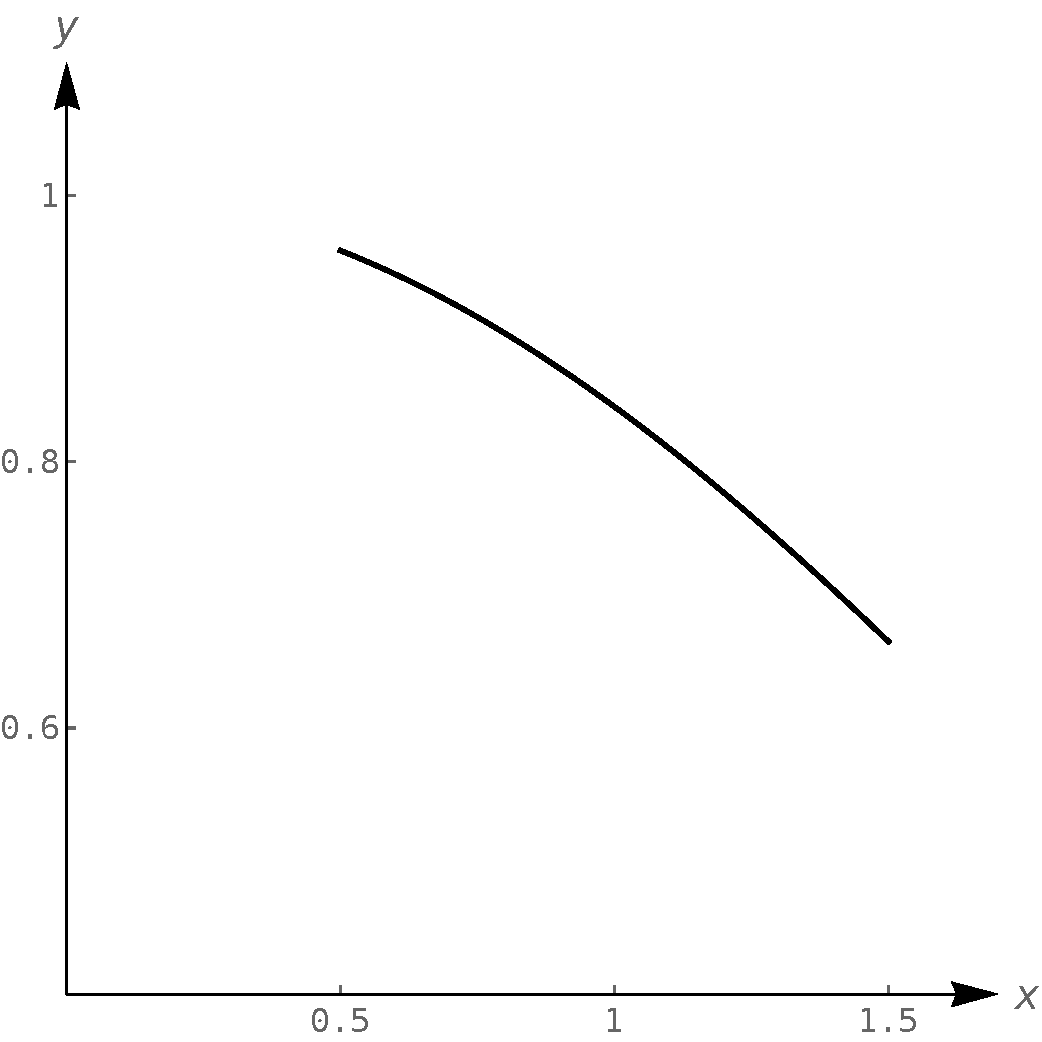
\includegraphics[width=0.4\textwidth]{fig_lim_1a}}
\qquad
\subfigure[\label{fig_lim_1b}]{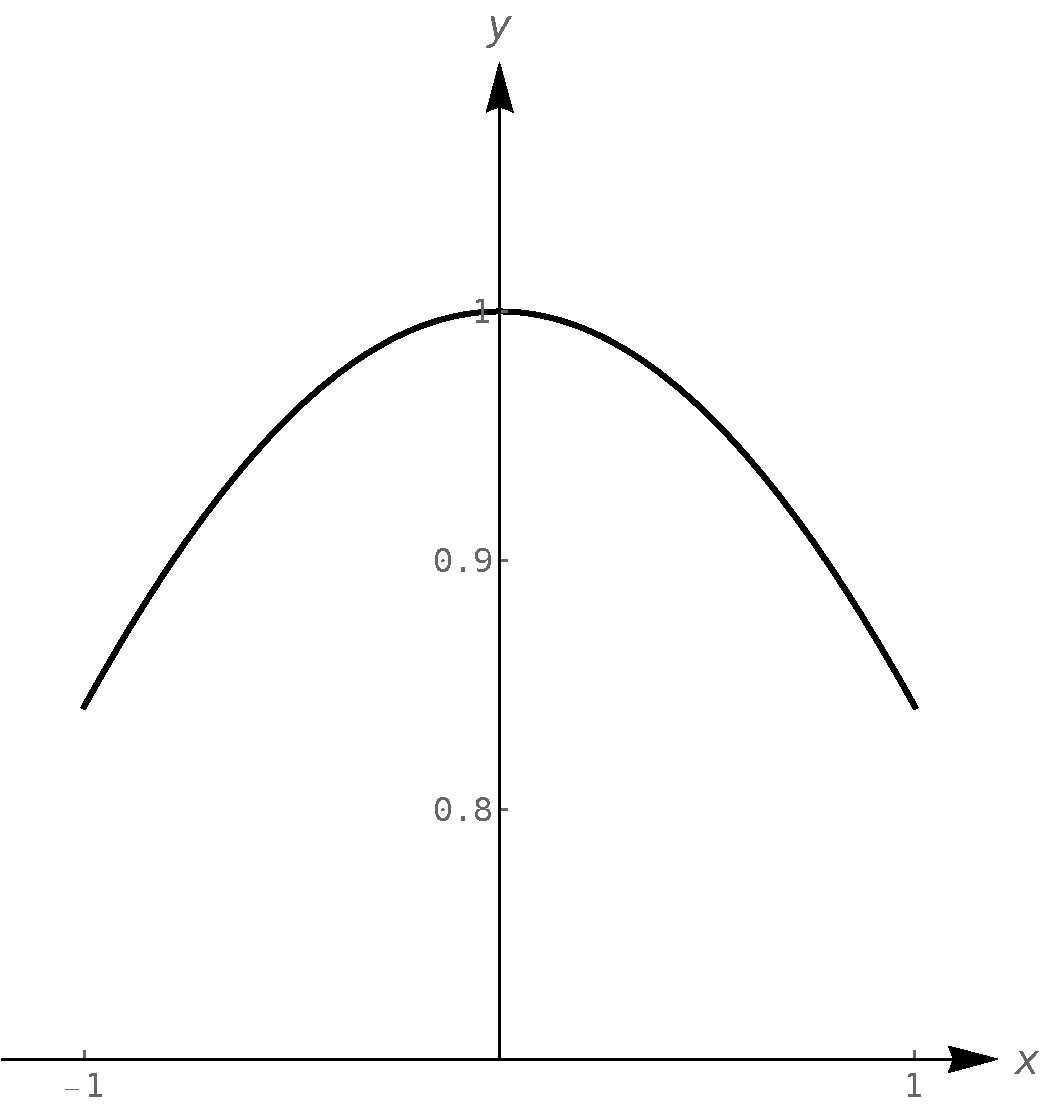
\includegraphics[width=0.4\textwidth]{fig_lim_1b} }
\caption{The graph of $y=\frac{\sin(x)}{x}$ near $x=1$ (a) and $x=0$ (b). }
\end{figure}



Finding a limit entails understanding how a function behaves near a particular value of $x$. Before continuing, it will be useful to establish some notation. Let $y=f(x)$; that is, let $y$ be a function of $x$ for some function $f$. The expression ``the limit of $y$ as $x$ approaches 1" describes a number, often referred to as $L$, that $y$ nears as $x$ nears 1. We write all this as 
$$\lim_{x\to 1} y = \lim_{x\to 1} f(x) = L.$$
 This is not a formal definition, but an intuitive one to settle the mind. It allows us to approximate limits both graphically and numerically.

For what concerns the function defined by Equation~\eqref{sinxopx}, we approximated graphically that 
$$\lim_{x\to 1} \frac{\sin (x)}{x} \approx 0.84 \quad \text{ and } \quad \lim_{x\to 0}\frac{\sin (x)}{x} \approx 1.
$$ 



\ifvc
\begin{example}\label{ex_limit2}
Graphically and numerically approximate the limit of $f(x)$ as $x$ approaches 0, where 
$$f(x) = \left\{\begin{array}{lcl} x+1, & \mbox{if} & x< 0, \\ -x^2+1, &\mbox{if} & x > 0. \end{array}\right.$$

\xhrulefill{gray}{2.5pt}Solution \xhrulefill{gray}{2.5pt}


We graph $f(x)$ and create a table of its values near $x=0$ to approximate the limit. Note that this is a piecewise defined function, so it behaves differently on either side of 0. Figure \ref{fig_lim_2a} shows a graph of $f(x)$, and on either side of 0 it seems the $y$ values approach 1. Note that $f(0)$ is not actually defined, as indicated in the graph with the open circle. Table~\ref{fig_lim_2b} shows values of $f(x)$ for values of $x$ near 0. It is clear that as $x$ takes on values very near 0, $f(x)$ takes on values very near 1. It turns out that if we let $x=0$ for either piece of $f(x)$, 1 is returned; this is significant and we will return to this idea later.

The graph and table allow us to say that $\lim_{x\to 0}f(x) \approx 1$; in fact, we are probably very sure it equals 1.

\begin{figure}[H]
  \centering
  \subfigure[\label{fig_lim_2a}]{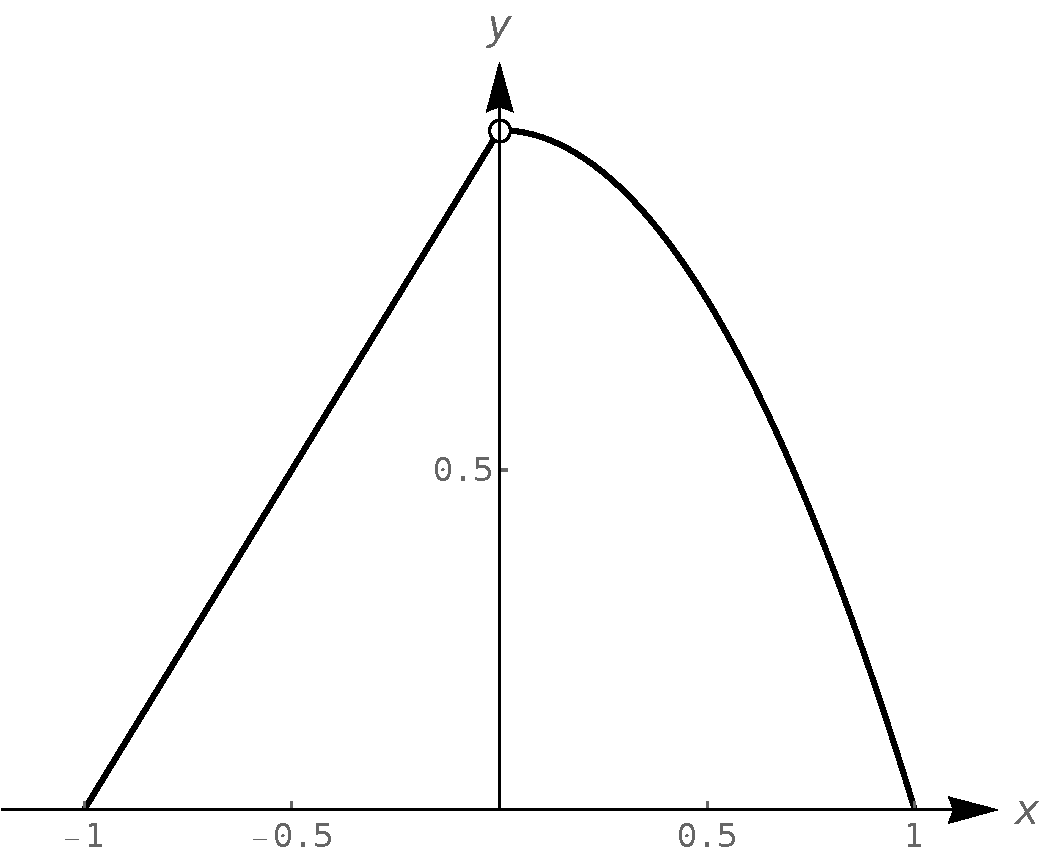
\includegraphics[width=0.43\textwidth]{fig_lim_2a}}%
  \qquad
  \subfigure[\label{fig_lim_2b}]{
  \renewcommand{\arraystretch}{1.5}
\begin{tabular}[b]{c|c}
$x$ & $f(x)$ \\ \hline\hline
-0.1 & 0.9 \\
 -0.01 & 0.99 \\
 -0.001 & 0.999 \\
 0.001 & 0.999999 \\
 0.01 & 0.9999 \\
 0.1 & 0.99
 \end{tabular}
 \renewcommand{\arraystretch}{1.}
  }
\caption{Graphically (a) and numerically (b) approximating a limit in Example \ref{ex_limit2}.}
\end{figure}

\end{example}
\fi



\subsection{Existence of limits}
A function may not have a limit for all values of $x$. That is, we cannot say $\lim\limits_{x\to c}f(x)=L$ for some numbers $L$ for all values of $c$, for there may not be a number that $f(x)$ is approaching. There are three common ways in which a limit may fail to exist. 
\begin{enumerate}
\item		The function $f(x)$ may approach different values on either side of $c$.
\item		The function may grow without upper or lower bound as $x$ approaches $c$.
\item		The function may oscillate as $x$ approaches $c$ without approaching a specific value.
\end{enumerate}

Each of these cases is illustrated in the following examples

\begin{example}
Let us consider the function
\begin{equation}
f(x) = \left\{\begin{array}{lcl} x^2-2x+3, &\mbox{if} & x\leq 1, \\ x, &\mbox{if} & x>1, \end{array}\right.
\label{eq_lim_1}
\end{equation}
and try to determine $\ds\lim_{x\to 1} f(x)$.



A graph of $f(x)$ around $x=1$ and a corresponding table are given in Figure \ref{fig_lim_3a} and \ref{fig_lim_3b}, respectively. It is clear that as $x$ approaches 1, $f(x)$ does not seem to approach a single number. Instead, it seems as though $f(x)$ approaches two different numbers. When considering values of $x$ less than 1, so approaching 1 from the left, it seems that $f(x)$ is approaching 2; when considering values of $x$ greater than 1 ,so approaching 1 from the right, it seems that $f(x)$ is approaching 1. Consequently, the limit does not exist since $f(x)$ is not approaching one value as $x$ approaches 1.



\begin{figure}[H]
  \centering
  \subfigure[\label{fig_lim_3a}]{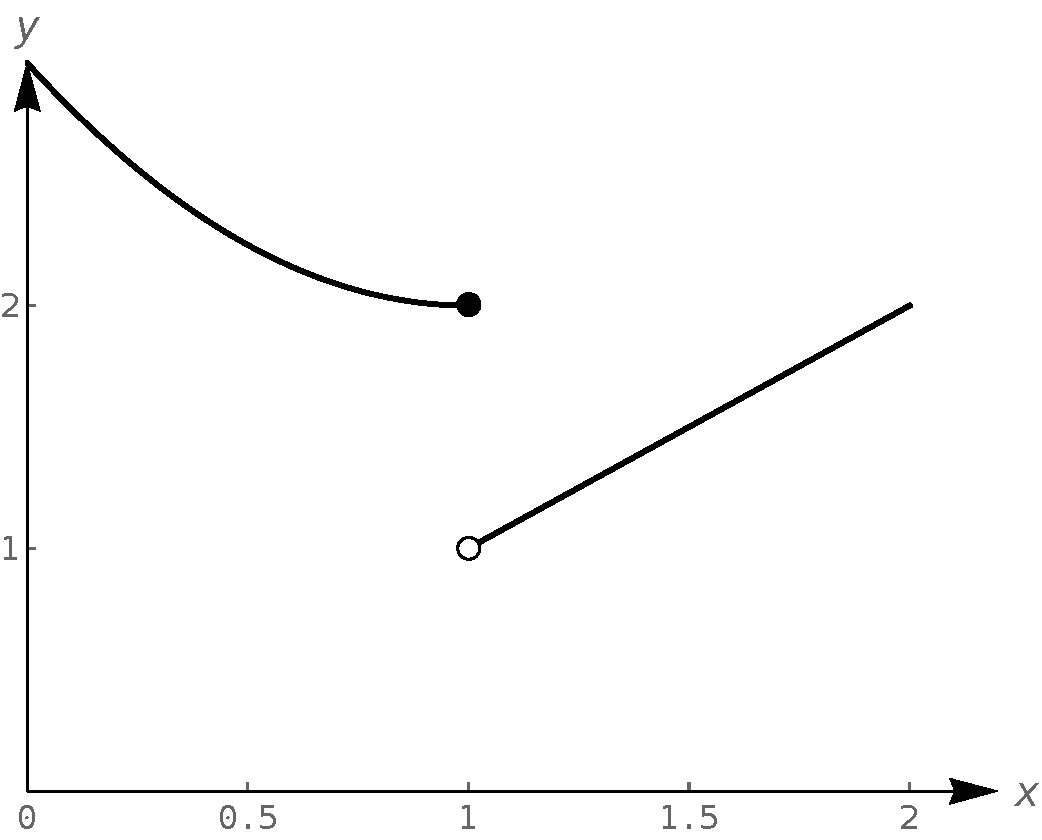
\includegraphics[width=0.43\textwidth]{fig_lim_3a}}%
  \qquad
  \subfigure[ \label{fig_lim_3b}]{
  \renewcommand{\arraystretch}{1.5}\begin{tabular}[b]{c|c}
$x$ & $f(x)$ \\ \hline\hline
 0.9 & 2.01 \\
 0.99 & 2.0001 \\
 0.999 & 2.000001 \\
 1.001 & 1.001 \\
 1.01 & 1.01 \\
 1.1 & 1.1
\end{tabular}
\renewcommand{\arraystretch}{1.}
  }
\caption{Graphically (a) and numerically (b) approximating $\ds\lim_{x\to 1} f(x)$ for $f$ given by Equation~\eqref{eq_lim_1}.}
\end{figure}

\end{example}


\begin{example}
\label{ex_no_limit2}
Let us now have a closer look at 
$$\ds\lim_{x\to 1} \dfrac{1}{(x-1)^2}\,.$$%


A graph and table of $f(x) = 1/(x-1)^2$ are given in Figure~\ref{fig_lim_4a} and \ref{fig_lim_4b}, respectively. Both show that as $x$ approaches 1, $f(x)$ grows larger and larger. Indeed, if $x$ is near 1, then $(x-1)^2$ is very small, and: 
$$\frac{1}{\text{very small number}} = \text{very large number}.$$
Since $f(x)$ is not approaching a single number, we conclude that $$\lim_{x\to 1}\frac{1}{(x-1)^2}$$ does not exist.

\begin{figure}[H]
  \centering
  \subfigure[\label{fig_lim_4a}]{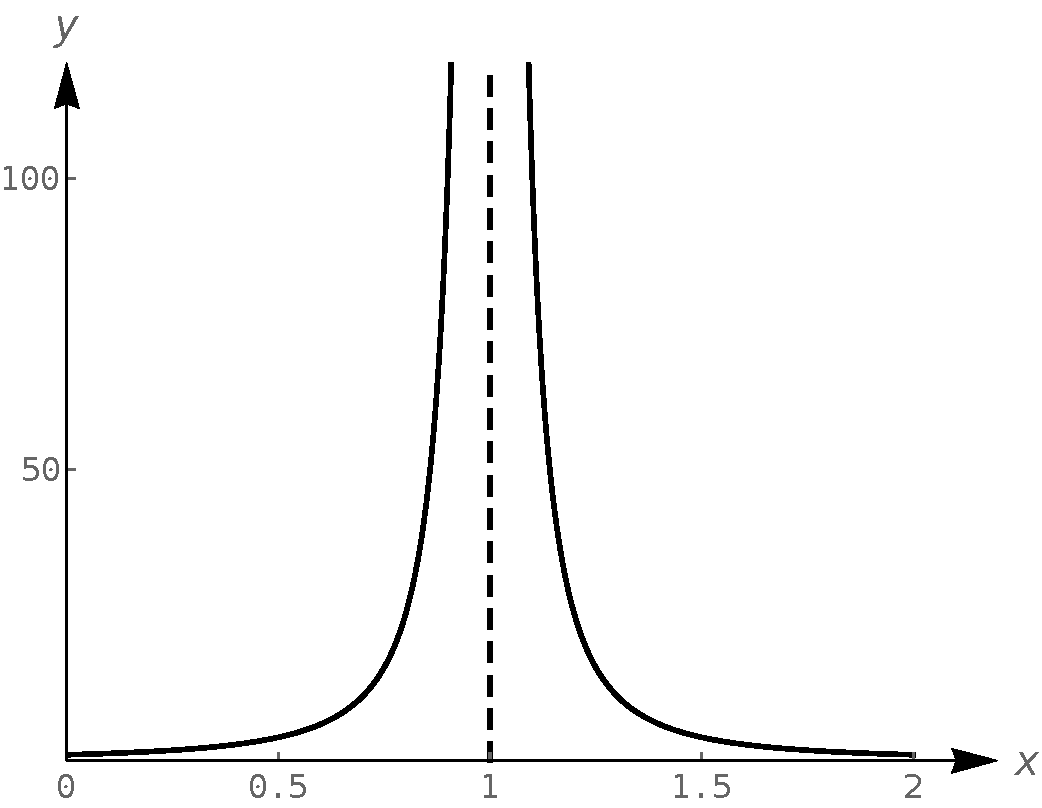
\includegraphics[width=0.43\textwidth]{fig_lim_4a}}%
  \qquad
  \subtable[\label{fig_lim_4b}]{\renewcommand{\arraystretch}{1.5}
  \begin{tabular}[b]{c|c}
$x$ & $f(x)$ \\ \hline\hline
 0.9 & 100. \\
 0.99 & 10000. \\
 0.999 & $1.\times 10^6$ \\
 1.001 & $1.\times 10^6$ \\
 1.01 & 10000. \\
 1.1 & 100.\\
\end{tabular}
\renewcommand{\arraystretch}{1.}}
\caption{Graphically (a) and numerically (b) approximating $\ds\lim_{x\to 1} \frac{1}{(x-1)^2}$.}
\end{figure}


\end{example}


\begin{example}
Let us finally explore why 
$$\ds\lim_{x\to 0}\sin\left(\dfrac{1}{x}\right)$$
does not exist.


For that purpose, Figure~\ref{fig_lim_5a} shows $f(x)$ on the interval $[-0.1,0.1]$; notice how $f(x)$ clearly seems to oscillate near $x=0$.   This is confirmed in Table~\ref{fig_lim_5b}, where we see $\sin(1/x)$ evaluated for values of $x$ near 0. As $x$ approaches 0, $f(x)$ does not appear to approach any value. It can be shown that in reality, as $x$ approaches 0, $\sin(1/x)$ takes on all values between $-1$ and 1 infinitely many times. Because of this oscillation, so the considered limit does not exist.





\begin{figure}[H]
  \centering
  \subfigure[\label{fig_lim_5a}]{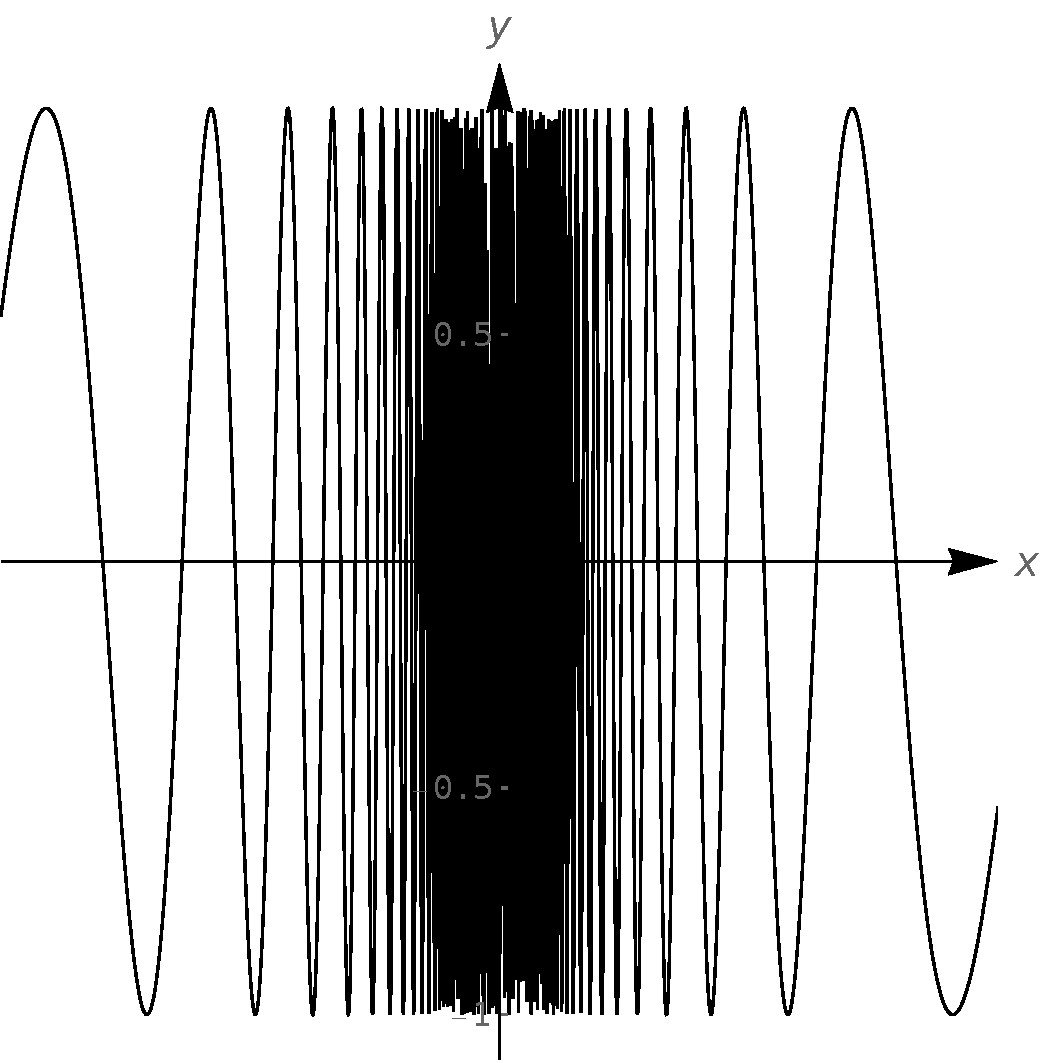
\includegraphics[width=0.43\textwidth]{fig_lim_5a}}
  \qquad
  \subtable[\label{fig_lim_5b}]{\renewcommand{\arraystretch}{1.5}\begin{tabular}[b]{c|c}
 $x$ & $\sin(1/x)$ \\ \hline\hline
0.1 & $-0.544021$ \\ 
0.01 & $-0.506366$ \\ 
0.001 & 0.82688 \\ 
0.0001 & $-0.305614$ \\ 
$1.\times 10^{-5}$ & 0.0357488 \\
 $1.\times 10^{-6}$ & $-0.349994$ \\ 
$1.\times 10^{-7}$ & 0.420548 
\end{tabular}\renewcommand{\arraystretch}{1.}}
\caption{Graphically (a) and numerically (b) approximating $\ds\lim_{x\to 0} \sin\left(\frac{1}{x}\right)$.}
\end{figure}

\end{example}

\ifcourse
\subsection{Limits of difference quotients}

Let $f(x)$ represent the position function, in metres, of some particle that is moving in a straight line, where $x$ is measured in seconds. Let us say that when $x=1$, the particle is at position 10 m, and when $x=5$, the particle is at 20 m. Another way of expressing this is to say 
$$f(1)=10 \quad \text{ and } \quad f(5) = 20.$$
Since the particle travelled 10 metres in 4 seconds, we can say the particle's average velocity was 2.5 m/s. We write this using a quotient of differences, or, a \textbf{difference quotient} (\textit{differentiequoti\"ent}): \index{difference quotient}\index[aut]{differentiequoti\"ent}
 $$\frac{f(5) - f(1)}{5-1} = \frac{10}4 = 2.5 \text{m/s}.$$
In fact, we are finding in this way the slope of the \textbf{secant line} (\textit{snijlijn})\index[aut]{snijlijn}\index{secant line} through those two points.

Now consider finding the average speed on another time interval. We again start at $x=1$, but consider the position of the particle $h$ seconds later. That is, consider the positions of the particle when $x=1$ and when $x=1+h$. The difference quotient is now 
\begin{equation}
\frac{f(1+h)-f(1)}{(1+h)-1} = \frac{f(1+h)-f(1)}h.
\label{eq_lim_2}
\end{equation}

Let now 
$$f(x) = -1.5x^2+11.5x;$$
for which it holds that $f(1)=10$ and $f(5) = 20$. We can compute this difference quotient for all values of $h$ except $h=0$, for then we get 0/0, an indeterminate form. For all values $h\neq 0$, the difference quotient computes the average velocity of the particle over an interval of time of length $h$ starting at $x=1$.  For small values of $h$, i.e., values of $h$ close to 0, we get average velocities over very short time periods and compute secant lines over small intervals (Figure \ref{fig_lim_6}). This leads us to wonder what the limit of the difference quotient is as $h$ approaches 0. That is, 
$$\lim_{h\to 0} \frac{f(1+h)-f(1)}{h} = \text{ ? }.$$





\begin{figure}
\centering
%\raisebox{0.5cm}{
\centerline{
\subfigure[]{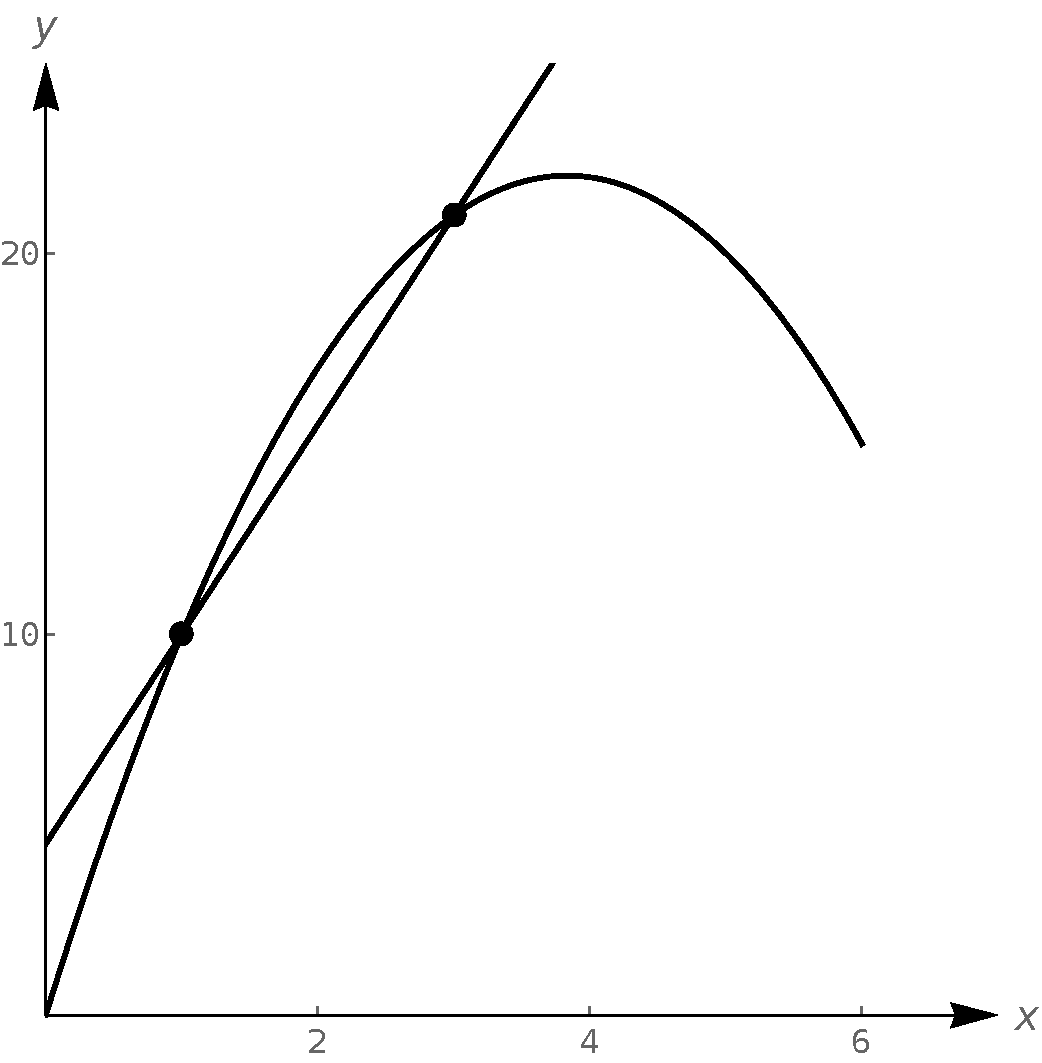
\includegraphics[width=0.3\textwidth]{fig_lim_6a}}
\qquad
\subfigure[]{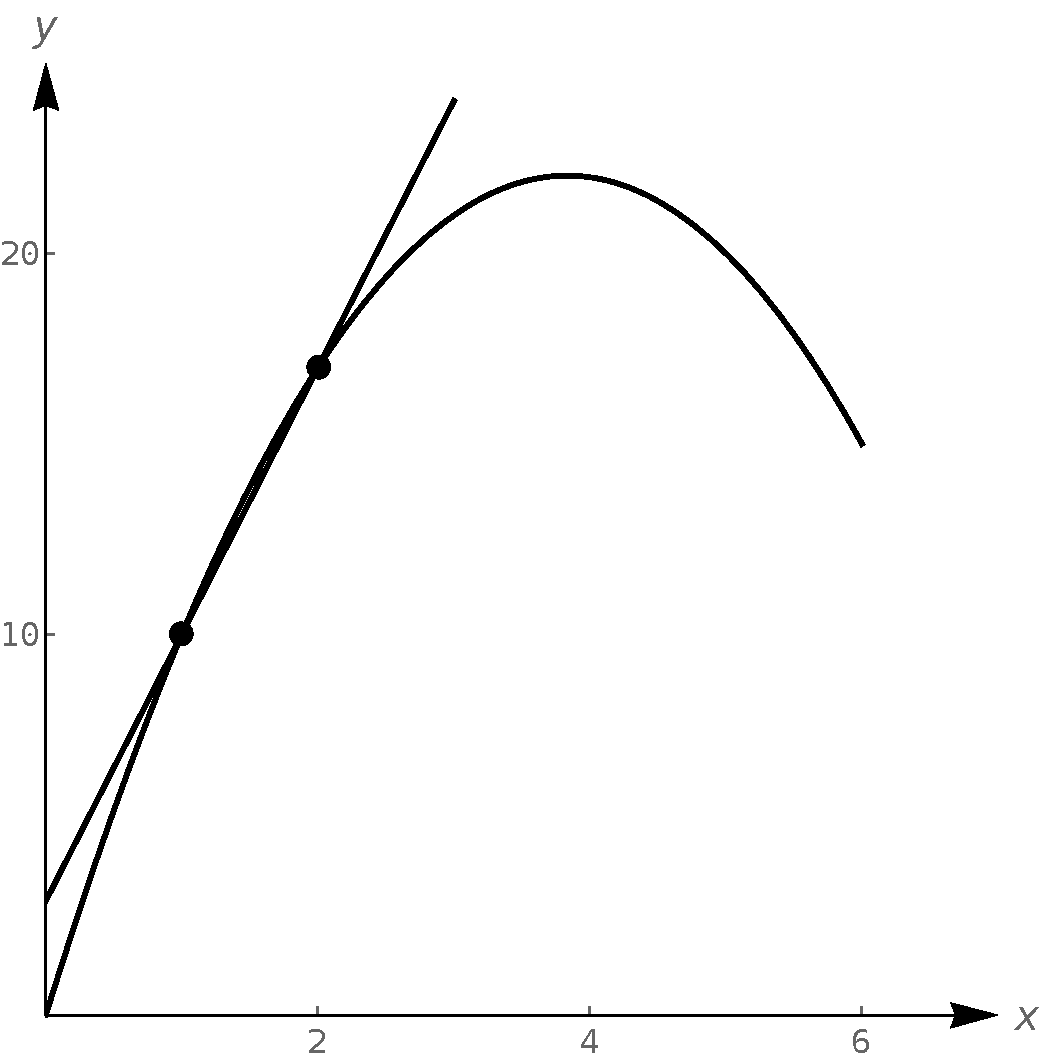
\includegraphics[width=0.3\textwidth]{fig_lim_6b} }
\qquad
\subfigure[]{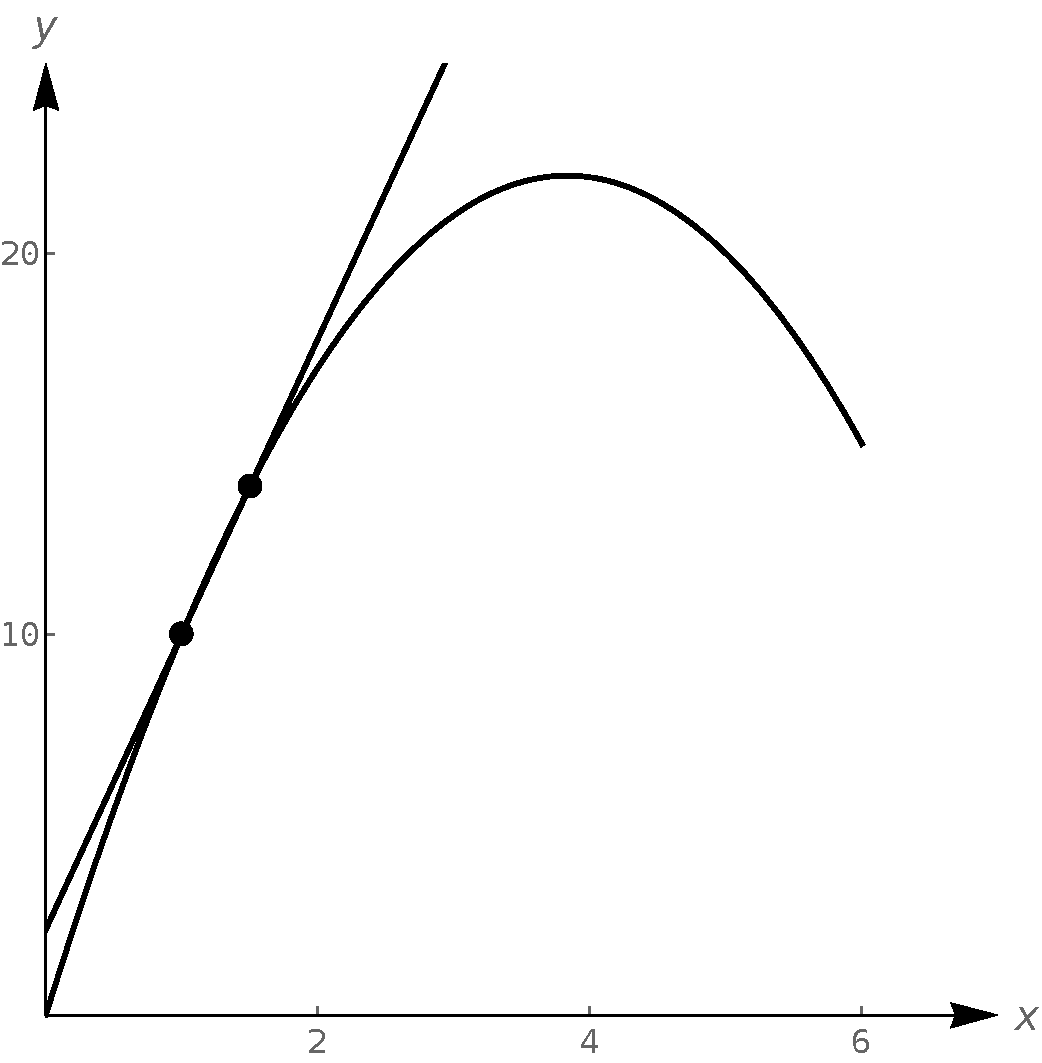
\includegraphics[width=0.3\textwidth]{fig_lim_6c} }
}
\caption{Secant lines of $f(x)$ at $x=1$ and $x=1+h$, for shrinking values of $h$. }
\label{fig_lim_6}
\end{figure}


As we do not yet have a true definition of a limit nor an exact method for computing it, we settle for approximating the value in Table~\ref{tab_lim_2}. This table gives us reason to assume the value of the limit is about 8.5. 

\begin{table}[H]
\caption{The difference quotient given by Equation~\eqref{eq_lim_2} evaluated at values of $h$ near 0.}
\label{tab_lim_2}
\centerline{
\renewcommand{\arraystretch}{1.5}
\begin{tabular}{c|c}
$h$ & $\dfrac{f(1+h)-f(1)}{h}$\vspace{1pt} \\ \hline\hline 
$-0.5$ & 9.25 \\
 $-0.1$ & 8.65 \\
 $-0.01$ & 8.515 \\
 0.01 & 8.485 \\ 
0.1 & 8.35 \\ 
0.5 & 7.75 \end{tabular}
\renewcommand{\arraystretch}{1}
}
\end{table}


Proper understanding of limits is key to understanding calculus. With limits, we can accomplish seemingly impossible mathematical things, like adding up an infinite number of numbers (and not get infinity) and finding the slope of a line between two points, where the two points are actually the same point. These are not just mathematical curiosities; they allow us to link position, velocity and acceleration together, connect cross-sectional areas to volume, find the work done by a variable force, and much more. 

In the next section we give the formal definition of the limit and begin our study of finding limits analytically.

\fi




\section{Epsilon-delta definition of a limit}\label{sec:limit_def}
This section introduces the formal definition of a limit, typically called the \textbf{epsilon-delta definition} (\textit{epsilon-delta definitie}), referring to the letters $\varepsilon$ and $\delta$ of the Greek alphabet.

\ifcalculus
Given a function $y=f(x)$ and an $x$-value, $c$, an informal way of describing a limit based on our findings in Section~\ref{sec:limit_intro} could be: 
\begin{quote}
The limit of the function $f$, as $x$ approaches $c$, is a value~$L$ if $y$ is near $L$  whenever $x$ is near $c$.
\end{quote}
Or formulated in a more quantitative way:

\begin{quote}
If $x$ is within a certain tolerance level of $c$, then the corresponding value $y=f(x)$ is within a certain tolerance level of $L$.
\end{quote}

Since the traditional notation for the $x$-tolerance is the lowercase Greek letter delta ($\delta$), and the $y$-tolerance is denoted by lowercase epsilon, ($\varepsilon$) we may reformulate our definition as:

\begin{quote}
If $x$ is within $\delta$ units of $c$, then the corresponding value of $y$ is within $\varepsilon$ units of $L$.
\end{quote}

Using the absolute value to express the tolerance `$x$ is within $\delta$ units of $c$' mathematically, i.e. as 
$$|x-c| < \delta\,, $$
we arrive at following formal statement to define a limit
$$
|x - c| < \delta \longrightarrow  |y - L| < \varepsilon\,.
$$
Note that $\delta$ and $\varepsilon$, being tolerances, can be any positive (but typically small) values. The full formal definition of a limit we arrive at in this way is given below. 

\fi

\ifvc
Given a function $y=f(x)$ and an $x$-value, $c$, an informal way of describing a limit based on our findings in Section~\ref{sec:limit_intro} could be: 
\begin{quote}
The limit of the function $f$, as $x$ approaches $c$, is a value~$L$ if $y$ is near $L$  whenever $x$ is near $c$.
\end{quote}
Or formulated in a more quantitative way:

\begin{quote}
If $x$ is within a certain tolerance level of $c$, then the corresponding value $y=f(x)$ is within a certain tolerance level of $L$.
\end{quote}

Since the traditional notation for the $x$-tolerance is the lowercase Greek letter delta ($\delta$), and the $y$-tolerance is denoted by lowercase epsilon, ($\varepsilon$) we may reformulate our definition as:

\begin{quote}
If $x$ is within $\delta$ units of $c$, then the corresponding value of $y$ is within $\varepsilon$ units of $L$.
\end{quote}

Using the absolute value to express the tolerance `$x$ is within $\delta$ units of $c$' mathematically, i.e. as 
$$|x-c| < \delta\,, $$
we arrive at following formal statement to define a limit
$$
|x - c| < \delta \longrightarrow  |y - L| < \varepsilon\,.
$$
Note that $\delta$ and $\varepsilon$, being tolerances, can be any positive (but typically small) values. The full formal definition of a limit we arrive at in this way is given below. 

\fi


\begin{definition}[The limit of a function $f$]\label{def:limit}
Let $I$ be an open interval containing $c$, and let $f$ be a function defined on $I$, except possibly at $c$. The limit of $f(x)$, as $x$ approaches $c$, is $L$, denoted by  
$$\displaystyle \lim_{x\rightarrow c} f(x) = L,$$
and means that given any $\varepsilon > 0$, there exists $\delta > 0$ such that for all $x$ in $I$, where $x\neq c$,  
if  $|x - c| < \delta$, then $|f(x) - L| < \varepsilon$.
\index{limit ! definition}\index[aut]{limiet ! definitie}
\end{definition}  



Note the order in which $\varepsilon$ and $\delta$ are given.  In the definition, the $y$-tolerance $\varepsilon$ is given first and then the limit will exist  if we can find an $x$-tolerance $\delta$ that works. \ifanalysis Note also that Definition~\ref{def:limit} basically requires that the point $c$ is a limit point (see Definition~\ref{def:open1D}). \fi \ifcourse The $(\varepsilon,\delta)$ definition is illustrated in Figure~\ref{fig_lim_7}.\fi

\ifvc
\begin{figure}[H]
	\begin{center}
			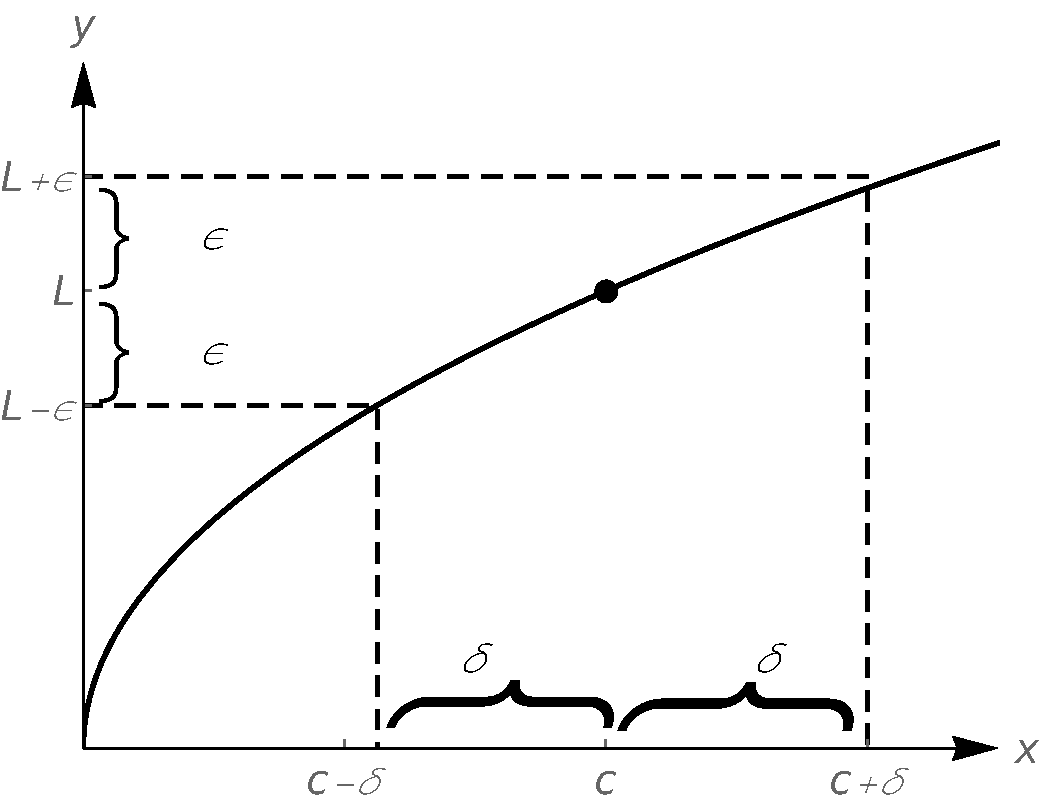
\includegraphics[width=0.5\textwidth]{fig_lim_7}
	\caption{Illustrating the $(\varepsilon,\delta)$ definition. }
	\label{fig_lim_7}
	\end{center}
\end{figure}
\fi

\ifcourse
\begin{figure}[H]
	\begin{center}
			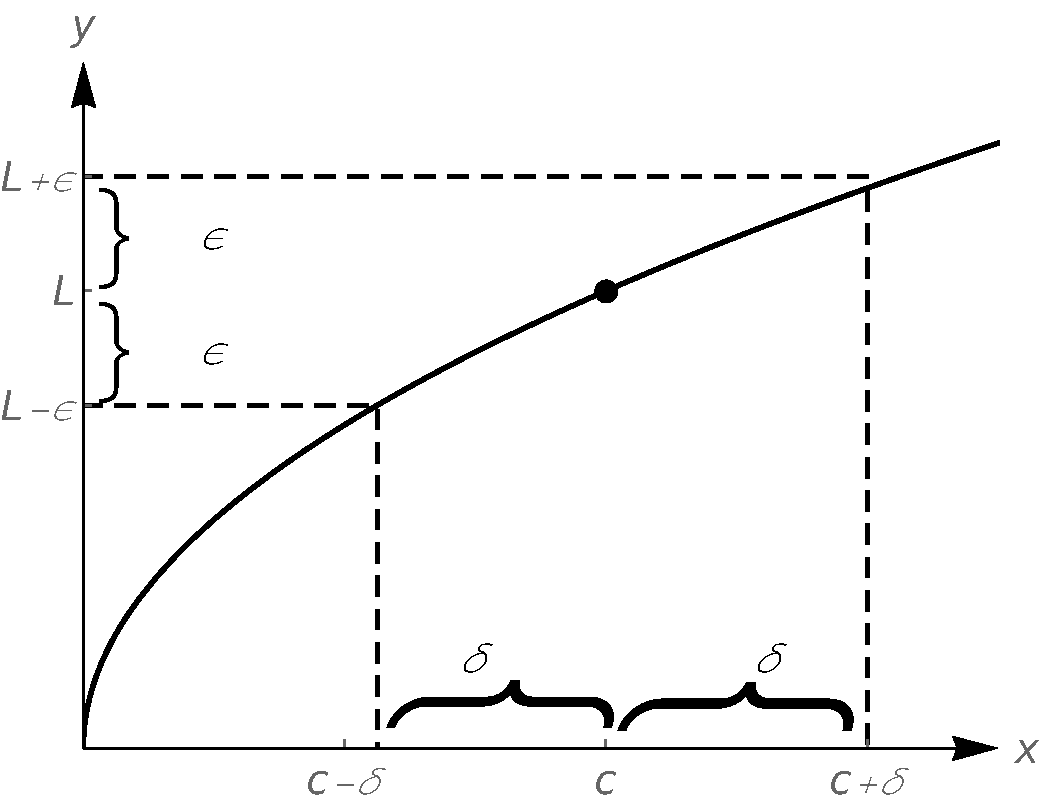
\includegraphics[width=0.5\textwidth]{fig_lim_7}
	\caption{Illustrating the $(\varepsilon,\delta)$ definition. }
	\label{fig_lim_7}
	\end{center}
\end{figure}
\fi



\ifcourse
\ifanalysis

Using logic operators only, Definition~\ref{def:limit} becomes
$$\displaystyle \lim_{x\rightarrow c} f(x) = L \quad \Leftrightarrow \quad \forall\,\varepsilon > 0, \exists \, \delta(\varepsilon) > 0  : \; \left(\forall x\in I\setminus\{c\}\,:\,
0<|x - c| < \delta \; \Rightarrow \; |f(x) - L| < \varepsilon\right)\,.$$

With the epsilon-delta definition of a limit in mind, we can easily show that there can be at most one limit of a function, as $x$ approaches $c$.

\begin{theorem}
Let $I$ be an open interval containing $c$, and let $f$ be a function defined on $I$, except possibly at $c$, then $f$ has at most one limit in $c$.
\end{theorem}

\begin{proof}
To prove this theorem, let us assume that $f$ has two limits in $c$; that is
$$
\lim_{x \rightarrow c} f(x) = L_1\text{ and } ~\lim_{x \rightarrow c} f(x) = L_2.
$$
Take $\varepsilon > 0$. Then, there exist $\delta_{1}(\varepsilon)$ and  $\delta_{2}(\varepsilon)$ for which it holds that
$$
\left|f(x)-L_1\right| < \varepsilon_1 \ \mbox{en} \ \left|f(x)-L_2\right| < \varepsilon_2
$$
for $x \in I$ if $ ~0 < \left|x-c\right| < \delta_1(\varepsilon)$ and  $0 < \left|x-c\right| < \delta_2(\varepsilon)$. Hence, for every such $x$ the following holds:
\begin{eqnarray*}
\left|L_1-L_2\right| & = & \left|L_1-f(x) + f(x)-L_2\right| \\
                     & \leq & \left|L_1-f(x)\right| + \left|f(x)-L_2\right| < \varepsilon_1+\varepsilon_2=\varepsilon.   
\end{eqnarray*}
Consequently, since $\varepsilon > 0$ was chosen arbitrarily, it follows that $L_1-L_2 = 0$.
\end{proof}


\fi
\fi
 
\ifanalysis
	\ifcourse
		\checkoddpage
\marginpar{\ifoddpage\hspace*{-1.5cm}\else\hspace*{0.25cm}\fi
\includegraphics[width=0.075\textwidth]{youtube}\\
\ifoddpage\hspace*{-1.75cm}\else\hspace*{0.1cm}\fi
\qrcode[height=1.75cm]{https://youtu.be/LZ9C-JQVtQc}
%\includegraphics[width=0.1\textwidth]{figures/Lim/epsilon_delta.png}
}
 \fi
 


An example will help us understand this definition.

\begin{example}\label {ex_compute_lim1}
Show that $\displaystyle \lim_{x\rightarrow 4} \sqrt{x} = 2 $.

\pagebreak
\xhrulefill{gray}{2.5pt}Solution \xhrulefill{gray}{2.5pt}

\ifcalculus 
Let us first try some numerical tolerances.  What if the $y$ tolerance is 0.5, or $\varepsilon =0.5$?  How close to 4 does $x$ have to be so that $y$ is within 0.5 units of 2?  In this case, we can proceed as follows:

 \[ \begin{array}{rrcccl}
&&&|y-2|& < & 0.5\\
\Leftrightarrow&-0.5 &<& y-2 &<& 0.5 \\
\Leftrightarrow&1.5 &<& y &<& 2.5 \\
\Leftrightarrow&1.5 &<& \sqrt{x} &<& 2.5 \\
\Leftrightarrow&1.5^2 &<& x &<& 2.5^2 \\
\Leftrightarrow&2.25 &<& x &<& 6.25 \\\end{array}\]

So, what is the desired $x$ tolerance?  Remember, we want to find a symmetric interval of $x$ values, namely
$4 - \delta < x < 4 + \delta$.  The lower bound of $2.25$ is $1.75$ units from 4; the upper bound of 6.25 is 2.25 units from 4. We need the smaller of these two distances; we must have $\delta < 1.75$ (Figure~\ref{fig_lim_8}). Consequently, given the $y$ tolerance $\varepsilon =0.5$, we have found an $x$ tolerance, $\delta < 1.75$, such that whenever $x$ is within $\delta$ units of 4, then $y$ is within $\varepsilon$ units of 2.  

\begin{figure}[H]
\centering
%\raisebox{0.5cm}{
\centerline{
\subfigure[]{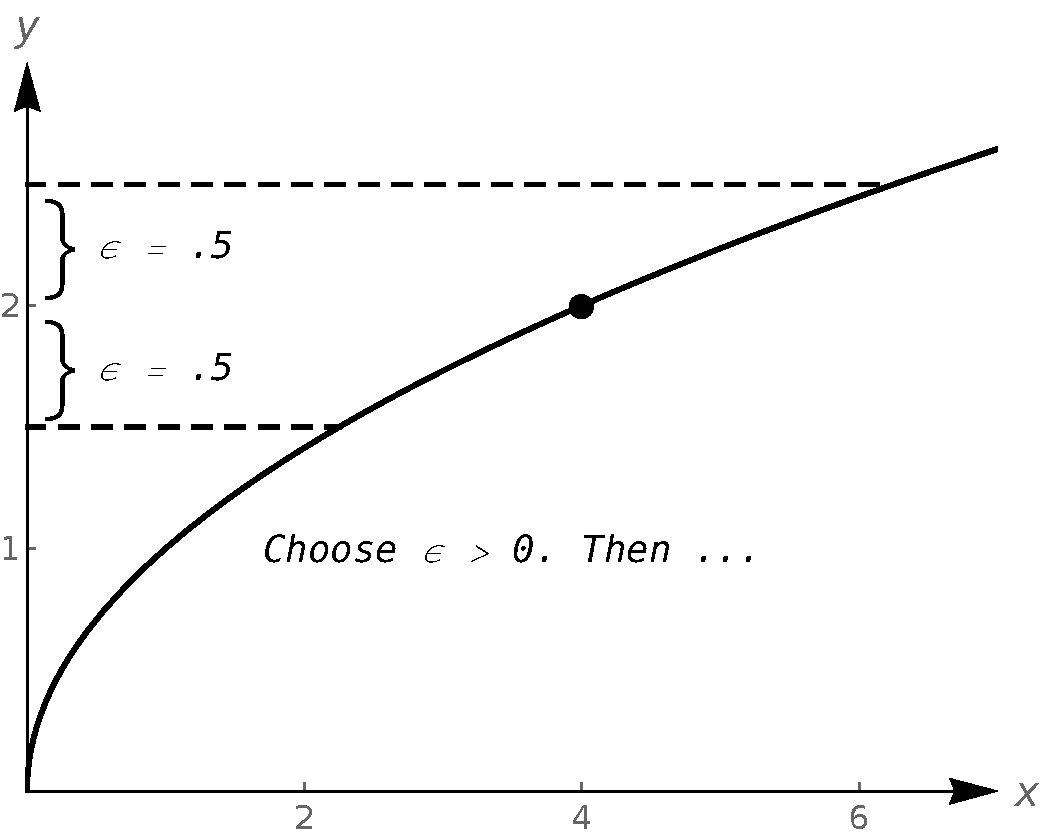
\includegraphics[width=0.4\textwidth]{fig_lim_8a}}
\qquad
\subfigure[]{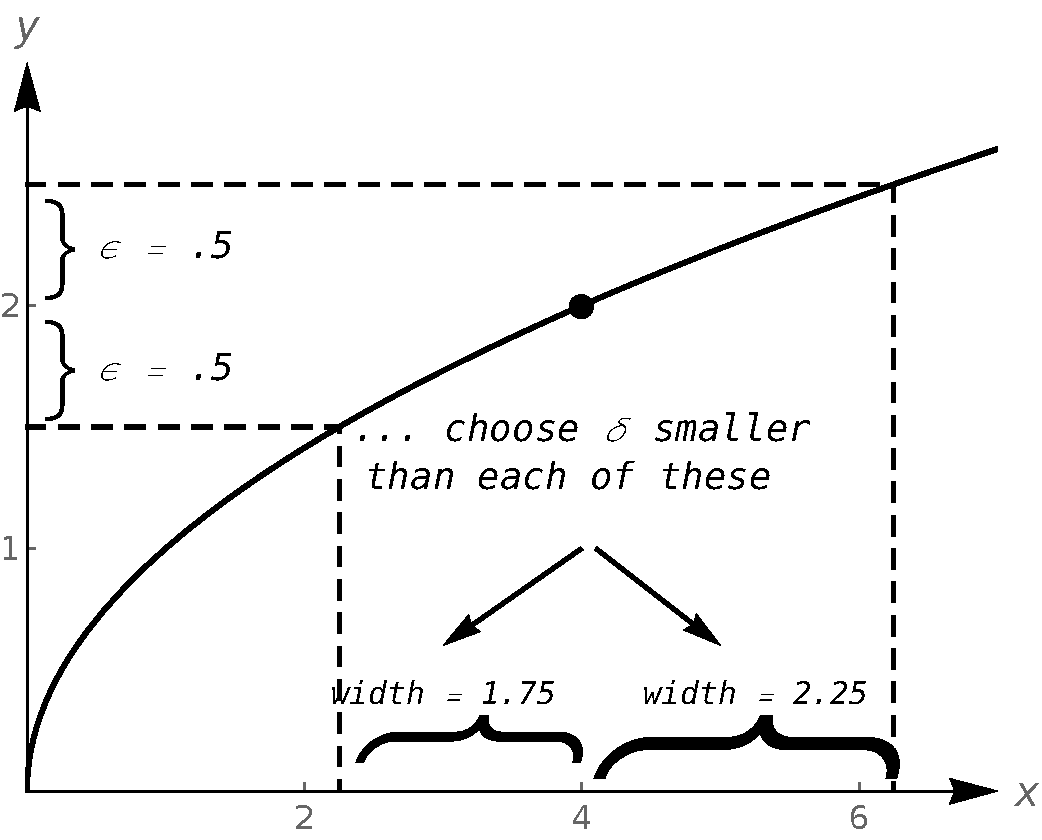
\includegraphics[width=0.4\textwidth]{fig_lim_8b} }
}
\caption{Illustrating the $(\varepsilon,\delta)$-process. }
\label{fig_lim_8}
\end{figure}


Let us now switch to general $\varepsilon$ and try to determine $\delta$ symbolically. \fi 
We start by assuming $y=\sqrt{x}$ is within $\varepsilon$ units of 2:
$$
\begin{array}{rrcccll}
&&&|y - 2| &<& \varepsilon \\
\Leftrightarrow&-\varepsilon &<& y - 2 &<& \varepsilon & \textrm{(Definition of absolute value.)}\\
\Leftrightarrow&-\varepsilon &<& \sqrt{x} - 2 &<& \varepsilon  & (y=\sqrt{x}.)\\
\Leftrightarrow&2 - \varepsilon &<& \sqrt{x}& <& 2+ \varepsilon & \textrm{ (Add 2.)}\\
\Leftrightarrow&(2 - \varepsilon)^2 &<& x &<& (2+ \varepsilon) ^2 &\textrm{ (Square all.)}\\
\Leftrightarrow&4 - 4\varepsilon + \varepsilon^2 &<& x &<& 4 + 4\varepsilon + \varepsilon^2 & \textrm{ (Expand.)}\\
\Leftrightarrow&4 - (4\varepsilon - \varepsilon^2) &<& x &<& 4 + (4\varepsilon + \varepsilon^2). & \textrm{ (Rewrite in the desired form.)}
\end{array}
$$


The desired form in the last step is ``$4-something < x < 4 +something$.''
Since we want this last interval to describe an $x$ tolerance around 4, we have that either $\delta < 4\varepsilon - \varepsilon^2$ or $\delta < 4\varepsilon + \varepsilon^2$, whichever is smaller: $$\delta < \min\{4\varepsilon - \varepsilon^2, 4\varepsilon + \varepsilon^2\}.$$  Since $\varepsilon > 0$, the minimum is $\delta < 4\varepsilon - \varepsilon^2$.  So, given an $\varepsilon$, we must set $\delta < 4\varepsilon-\varepsilon^2$. 



So given any $\varepsilon >0$, set $\delta < 4\varepsilon - \varepsilon^2$. Then if $|x-4|<\delta$ (and $x\neq 4$), it holds that $|f(x) - 2| < \varepsilon$, clearly satisfying the definition of the limit.  We have shown formally that $\displaystyle \lim_{x\rightarrow 4} \sqrt{x} = 2 $. We can check this for $\varepsilon=0.5$. In that case, the formula gives $\delta < 4(0.5) - (0.5)^2 = 1.75$. 
\end{example}


% \begin{example}\label{ex_compute_lim2}
% Show that $\displaystyle \lim_{x\rightarrow 2} x^2 = 4$.

% \pagebreak
% \xhrulefill{gray}{2.5pt}Solution \xhrulefill{gray}{2.5pt}

% \ifcalculus Let us do this example symbolically from the start. \fi Let $\varepsilon > 0$ be given; we want $|y-4| < \varepsilon$, i.e.,  $|x^2-4| < \varepsilon$.  How do we find $\delta$ such that when $|x-2| < \delta$, we are guaranteed that $|x^2-4|<\varepsilon$?% for some $\delta$ (in terms of $\varepsilon$)?

% This is a bit trickier than Example~\ref{ex_compute_lim1}, but let us start by noticing that 
% $|x^2-4| = |x-2|\,|x+2|$.  Consider:\\
% \begin{equation} |x^2-4| < \varepsilon \Longrightarrow |x-2|\,|x+2| < \varepsilon \Longrightarrow |x-2|< \dfrac{\varepsilon}{|x+2|}  .\label{eq:limit1}\end{equation} 
% Could we not just set 
% $$\displaystyle \delta = \frac{\varepsilon}{|x+2|}?$$  

% Yet, $\delta$ must be a constant value.  Still, remember that $\varepsilon$ is supposed to be a small number, which implies that $\delta$ will also be a small value.  In particular, we can (probably) assume that $\delta < 1$.  If this is true, then $|x-2| < \delta$ would imply that $|x-2| < 1$, giving $1 < x < 3$.  

% Now, back to the fraction $ \varepsilon/|x+2|$.  If $1<x<3$, then $3<x+2<5$.  Taking reciprocals, we have 
% $$
% \frac15 < \frac1{|x+2|} < \frac 13\,,
% $$
% which implies 
% $$
% \frac15 < \frac1{|x+2|}
% $$
% which on its turn implies after multiplying both sides with $\varepsilon>0$:
% \begin{equation}
% \frac\epsilon5<\frac{\varepsilon}{|x+2|}\,.\label{eq:limit2}
% \end{equation}


% This suggests that we set $\delta < \varepsilon/5$. To see why, let consider what follows when we assume $|x-2|<\delta$:


% $$
% \begin{array}{rrcll}
% &|x - 2| &<& \delta &\\
% \Leftrightarrow&|x - 2| &<& \dfrac{\varepsilon}{5}&  \text{(Our choice of $\delta$.)}\\
% \Leftrightarrow&|x - 2|\,|x + 2| &<& |x + 2|\,\frac{\varepsilon}{5}&  \text{(Multiply by $|x+2|$.)}\\
% \Leftrightarrow&|x^2 - 4|&<& |x + 2|\,\dfrac{\varepsilon}{5}&  \text{(Combine left side.)}\\
% \Leftrightarrow&|x^2 - 4|&<& |x + 2|\,\dfrac{\varepsilon}{5}< |x + 2|\,\dfrac{\varepsilon}{|x+2|}=\varepsilon &  
% \text{(Using (\ref{eq:limit2}) as long as $\delta <1$.)}
% \end{array}
% $$
% \normalsize

% We have arrived at $|x^2 - 4|<\varepsilon$ as desired.  Note again, in order to make this happen we needed $\delta$ to first be less than 1.  That is a safe assumption; we want $\varepsilon$ to be arbitrarily small, forcing $\delta$ to also be small. 

% We have also picked $\delta$ to be smaller than necessary. We could get by with a slightly larger $\delta$, as shown in Figure \ref{fig_lim_8}. The dashed outer lines show the boundaries defined by our choice of $\varepsilon$. The dotted inner lines show the boundaries defined by setting $\delta =  \varepsilon/5$. Note how these dotted lines are within the dashed lines. That is perfectly fine; by choosing $x$ within the dotted lines we are guaranteed that $f(x)$ will be within $\varepsilon$ of 4.%If the value we eventually used for $\delta$, namely $\varepsilon/5$, is not less than 1, this proof won't work.  For the final fix, we instead set $\delta$ to be the minimum of 1 and $\varepsilon/5$. This way all calculations above work.  



% In summary, given $\varepsilon > 0$, set $\delta=\varepsilon/5$.  Then $|x - 2| < \delta$ implies 
% $|x^2 - 4|< \varepsilon$ as desired.  This shows that $\displaystyle \lim_{x\rightarrow 2} x^2 = 4 $. Figure \ref{fig_lim_8} gives a visualization of this; by restricting $x$ to values within $\delta =  \varepsilon/5$ of 2, we see that $f(x)$ is within $\varepsilon$ of $4$.

% \begin{figure}[H]
% 	\begin{center}
% 			\includegraphics[width=0.5\textwidth]{fig_lim_8}
% 	\caption{Choosing $\delta =  \varepsilon/5$ in Example \ref{ex_compute_lim2}. }
% 	\label{fig_lim_8}
% 	\end{center}
% \end{figure}



% \end{example}

Make note of the general pattern exhibited in the last example. In some sense, each starts out backwards. That is, while we want to
\begin{enumerate}
	\item start with $|x-c|<\delta$ and conclude that
	\item $|f(x)-L|<\varepsilon$,
\end{enumerate}
we actually start by assuming 
\begin{enumerate}
	\item $|f(x)-L|<\varepsilon$, then perform some algebraic manipulations to give an inequality of the form
	\item $|x-c|<$ something.
\end{enumerate} 
%then perform some algebraic manipulations to transform that inequality into an inequality where the ``less than'' side is $|x-c|$. 
When we have properly done this, the something on the greater than side of the last inequality becomes our $\delta$ we are looking for. Once we have such a $\delta$, we can formally start with $|x-c|<\delta$ and use algebraic manipulations to conclude that $|f(x)-L|<\varepsilon$. This is once more illustrated in an example. 

% \begin{example}\label{ex_compute_lim4}
% Prove that $\ds \lim_{x\rightarrow 1}(x^3-2x) = -1$.


% \xhrulefill{gray}{2.5pt}Solution \xhrulefill{gray}{2.5pt}


% We start by considering $|f(x) - (-1)| < \varepsilon$:
% $$
% \begin{array}{rrcll}
% &|f(x)-(-1)| &<& \varepsilon&\\
% \Leftrightarrow&|x^3-2x + 1|&<& \varepsilon & \text{(Factor.)}\\
% \Leftrightarrow&|(x-1)(x^2+x-1)|&<& \varepsilon &\\
% \Leftrightarrow&|x-1| &<&\frac{\varepsilon}{|x^2+x-1|}.&\label{eq:lim4}
% \end{array}
% $$
% We are at the phase of saying that $|x-1|<$ something, where something $=\varepsilon/|x^2+x-1|$. We want to turn that something into $\delta$.

% Since $x$ is approaching 1, we are safe to assume that $x$ is between 0 and 2. Mathematically, this means that the following holds:
% $$
% \begin{array}{rrcccl}
% &0&<&x&<&2  \\
% \Rightarrow&0&<&x^2&<&4.\qquad\text{(Square each term.)}
% \end{array}
% $$
% Since $0<x<2$, we can add $0$, $x$ and $2$, respectively, to each part of the inequality and maintain the inequality.
% $$
% \begin{array}{rrcccl}
% &0&<& x^2+x&<6 &\\
% \Leftrightarrow&-1&<& x^2+x-1&<5&
% \end{array}
% $$

% In Equation \eqref{eq:lim4}, we wanted $|x-1|<\varepsilon/|x^2+x-1|$. The above shows that given any $x$ in $[0,2]$, we know that 
% $$
% x^2+x-1 < 5
% $$
% from which, upon rearranging terms, we infer
% $$
% \frac15 < \frac{1}{x^2+x-1}\,,
% $$
% which implies
% \begin{equation}
% \frac{\varepsilon}5 < \frac{\varepsilon}{x^2+x-1}\,.\label{eq:lim4b}
% \end{equation}
% So we choose $\delta < \varepsilon/5$ and can then start the formal proof.

% Given $\varepsilon$, let $\delta < \varepsilon/5$. We want to show that when $|x-1|<\delta$, then $|(x^3-2x)-(-1)|<\varepsilon$. We start with $|x-1|<\delta$:
% $$
% \begin{array}{rrcll}
% &|x-1| &<& \delta& \\
% \Leftrightarrow&|x-1| &<& \dfrac{\varepsilon}5&\\
% \Leftrightarrow&|x-1| &<& \dfrac\epsilon5 < \dfrac{\varepsilon}{|x^2+x-1|} & \text{(For $x$ near 1, from Equation \eqref{eq:lim4b})}\\
% \Leftrightarrow&|x-1|\cdot |x^2+x-1| &<& \varepsilon&\\
% \Leftrightarrow&|x^3-2x+1| &<& \varepsilon&\\
% \Leftrightarrow&|(x^3-2x)-(-1)| &<&\varepsilon&,
% \end{array}
% $$
% which is what we wanted to show. Thus $\ds \lim_{x\to 1}(x^3-2x) = -1$.
% \end{example}




\begin{example}
Prove that $\displaystyle \lim_{x\rightarrow 0} e^x = 1 $.

\xhrulefill{gray}{2.5pt}Solution \xhrulefill{gray}{2.5pt}


Symbolically, we want to take the equation $|e^x - 1| < \varepsilon$ and unravel it to the form $|x-0| < \delta$.  Hence:
$$
\begin{array}{rrcccll}
&&&|e^x - 1| &<& \varepsilon&\\
\Leftrightarrow&-\varepsilon &<& e^x - 1 &<& \varepsilon&\\
\Leftrightarrow&1-\varepsilon &<& e^x &<& 1+\varepsilon & \qquad \textrm{(Add 1.)}\\
\Leftrightarrow&\ln(1-\varepsilon) &<& x &<& \ln(1+\varepsilon) & \qquad \textrm{(Take natural logs.)}\\
\end{array}
$$
There is a caveat here.  If it happens that $\varepsilon \ge 1$, then $\ln(1-\varepsilon)$ would be undefined!  The way to work around this is to simply define a new epsilon, denoted $\epsilon_1$, that is guaranteed to be smaller than the original epsilon and less than 1, e.g.\ $\epsilon_1 = \min\{\varepsilon, 1/2\}$. Anyhow, let us continue now under the assumption that $\varepsilon<1$, so that $\ln (1-\varepsilon)$ is defined. 

Moreover, since $\ln (1-\varepsilon) <0$, we consider its absolute value, and consequently, we can then set $\delta$ to be the minimum of $|\ln(1-\varepsilon)|$ and $\ln(1+\varepsilon)$; i.e.,  
$$\delta = \min\{|\ln(1-\varepsilon)|, \ln(1+\varepsilon)\} = \ln(1+\varepsilon).$$  


Now, we work through the actual the proof:
$$
\begin{array}{rrcccl}
&&&|x - 0|&<&\delta\\
\Leftrightarrow&-\delta &<& x &<& \delta   \\
\Leftrightarrow&-\ln(1+\varepsilon) &<& x &<& \ln(1+\varepsilon). \\  
\Leftrightarrow&\ln(1-\varepsilon) &<& x &<& \ln(1+\varepsilon).  \qquad\text{(Since $\ln(1-\varepsilon) < -\ln(1+\varepsilon)$).}
\end{array}
$$

The above line is true by our choice of $\delta$ and by the fact that since $|\ln(1-\varepsilon)|>\ln(1+\varepsilon)$ and $\ln(1-\varepsilon)<0$, we know $\ln(1-\varepsilon) < -\ln(1+\varepsilon )$. That is; $\ln(1-\varepsilon)$ decreases much more rapidly to $-\infty$ for $0<\varepsilon<1$ than $\ln(1+\varepsilon)$ increases to $+\infty$ (see Section~\ref{sec_exponential}).

$$
\begin{array}{rrcccll}
&1-\varepsilon &<& e^x &<& 1+\varepsilon &  \textrm{(Exponentiate.)}\\
\Leftrightarrow&-\varepsilon &<& e^x - 1 &<& \varepsilon &  \textrm{(Subtract 1.)}\\
%-\varepsilon &<& e^x - 1 &<& \varepsilon & \qquad \textrm{(Since}\; \epsilon_1 \le \varepsilon)\\
\end{array}
$$

In summary, given $\varepsilon > 0$, let $\delta = \ln(1+\varepsilon)$. Then $|x - 0| < \delta$ implies $|e^x - 1|< \varepsilon$ as desired.  We have shown that $\displaystyle \lim_{x\rightarrow 0} e^x = 1 $.
\end{example}


We may as well use the epsilon-delta definition to show that a limit does not exist. 

\begin{example}
Prove that 
$$ \dlim_{x\rightarrow 0} \cos\left(\dfrac{1}{x}\right) $$ 
does not exist.


\xhrulefill{gray}{2.5pt}Solution \xhrulefill{gray}{2.5pt}

Suppose that $\dlim_{x\rightarrow 0} \cos\left(x^{-1}\right)=L$ and choose $\varepsilon=1/2$. Then, according to the epsilon-delta definition there exists a number $\delta > 0$ such that 
\[
\quad 0<|x|<\delta \quad \Rightarrow  \quad \left|\cos\left(\dfrac{1}{x}\right)-L\right|<\dfrac{1}{2}\cdot
\]
for all $x \in \mathbb{R}_0$. Now, consider  $n\in \mathbb{N}$ such that $\frac{1}{2n\pi}<\delta$. Substituting $x=\frac{1}{2n\pi}$ in the last inequality yields
\[ |\cos (2n\pi)-L|=|1-L|<\dfrac{1}{2} \quad \Rightarrow \quad \dfrac{1}{2}<L<\dfrac{3}{2}\,,\]

whereas choosing $x=\frac{1}{(2n+1)\pi}$, we arrive at 
\[ |\cos\left((2n+1)\pi\right)-L|=|-1-L|<\dfrac{1}{2} \quad \Rightarrow \quad -\dfrac{3}{2}<L<-\dfrac{1}{2}\, .\]

This last two inequalities are contradicting each other, so conclude that the limit does not exist. 
\end{example}




In the light of the examples we examined, it should be clear that $(\varepsilon,\delta)$-proofs are long and difficult to do. Luckily, in the next section we will learn some theorems that allow us to evaluate limits analytically, that is, without using the $(\varepsilon,\delta)$-definition explicitly.



\fi



\section{Finding limits analytically}
\label{sec:berekenen_lim}
\ifcourse Recognizing that $(\varepsilon,\delta)$-proofs are cumbersome, this section gives a series of theorems which allow us to find limits much more quickly and intuitively. \fi
\ifvc This section gives a series of theorems which allow us to find limits quickly and intuitively. \fi
%\vskip \baselineskip
\subsection{Properties of limits}
 The following properties of limits indicate that already established limits do behave nicely. For that purpose, let $b$, $c$, $L_1$ and $L_2$ be real numbers, let $n$ be a positive integer, and let $f$ and $g$ be functions defined on an open interval $I$ containing $c$ with the following limits: \index{limit!properties}
$$\lim_{x\to c}f(x) = L_1 \qquad \text{\ and\ }\qquad \lim_{x\to c} g(x) = L_2.$$


Then, the following limits hold.
\begin{enumerate}
\item \parbox{120pt}{\textbf{Constants}:} $\displaystyle \lim_{x\to c} b = b$
\item	\parbox{120pt}{\textbf{Identity}:}						$\displaystyle \lim_{x\to c} x = c$
\item	\parbox{120pt}{\textbf{Sums/Differences}:} $\displaystyle \lim_{x\to c}(f(x)\pm g(x)) = L_1\pm L_2$
\item	\parbox{120pt}{\textbf{Scalar multiples}:}	$\displaystyle \lim_{x\to c} b\, f(x) = bL_1$
\item	\parbox{120pt}{\textbf{Products}:}	$\displaystyle \lim_{x\to c} f(x) g(x) = L_1L_2$
\item	\parbox{120pt}{\textbf{Quotients}:} $\displaystyle \lim_{x\to c} \frac{f(x)}{g(x)} = \frac{L_1}{L_2}$, ($L_2\neq 0)$
\item	\parbox{120pt}{\textbf{Powers}:} 	$\displaystyle \lim_{x\to c} f(x)^n = L_1^n$
\item	\parbox{120pt}{\textbf{Roots}:}		$\displaystyle \lim_{x\to c} \sqrt[n]{f(x)} = \sqrt[n]{L_1}$, where $f(x)\geq 0$ on $I$ if $n$ is even.
\end{enumerate}

For what concerns function composition, we get
 $$\ds \lim_{x\to c}g(f(x)) = N\,,$$
provided
$$\lim_{x\to c}f(x) = M,\qquad\ \lim_{x\to M} g(x) = N\qquad \text{\ and\ }\qquad g(M)=N .$$

\ifcourse
\ifanalysis

By relying on the epsilon-delta definition of a limit (Definition~\ref{def:limit}), these properties can be shown rather easily. We illustrate this for
$$
\displaystyle \lim_{x\to c}(f(x)+ g(x)) = L_1+ L_2.
$$
Let us assume that 
\[ \dlim_{x\rightarrow x_0}f(x)=L_1 \qquad \mbox{and} \qquad \dlim_{x\rightarrow x_0}g(x)=L_2 .\]

From the epsilon-delta definition of a limit, we then have that
\[  \forall \, \varepsilon >0 , \; \exists \, \delta_1(\varepsilon)>0 : \quad 0<|x-x_0|<\delta_1 \quad \Rightarrow \quad |f(x)-L_1|<\varepsilon \]
\[ \forall \, \varepsilon >0 , \; \exists \, \delta_2(\varepsilon)>0 : \quad 0<|x-x_0|<\delta_2 \quad \Rightarrow \quad |g(x)-L_2|<\varepsilon .\]

Moreover, it holds that
\[ |f(x)+g(x)-(L_1+L_2)|\leq|f(x)-L_1|+|g(x)-L_2|<2\varepsilon .\]

Let $\varepsilon'=2\varepsilon$ and $\delta'(\varepsilon)=\mbox{min}\{\delta_1(\varepsilon),\delta_2(\varepsilon)\}$, then it holds that
\[\forall \, \varepsilon'>0, \; \exists \, \delta'(\varepsilon')>0: \quad 0<|x-x_0|<\delta' \quad \Rightarrow \quad |f(x)+g(x)-(L_1+L_2)|<\varepsilon' ,\]
from which
\[ \dlim_{x\rightarrow x_0} [f(x)+g(x)]=L_1+L_2=\dlim_{x\rightarrow x_0}f(x) +\dlim_{x\rightarrow x_0}g(x) \, .\]

\fi
\fi

We use these properties in the following example.

\begin{example}\label{ex_basic_limit_1}
Let $$\lim_{x\to 2} f(x)=2,\quad\lim_{x\to 2} g(x) = 3\quad \text{\ and \ }\quad p(x) = 3x^2-5x+7.$$ Find the following limits:

\noindent\begin{minipage}[t]{.5\textwidth}
\begin{enumerate}
\item		$\ds \lim_{x\to 2} \big(f(x) + g(x)\big)$
\item		$\ds \lim_{x\to 2} \big(5f(x) + g(x)^2\big)$
\end{enumerate}
\end{minipage}
\begin{minipage}[t]{.5\textwidth}
\begin{enumerate}\addtocounter{enumi}{2}
\item		$\ds \lim_{x\to 2} p(x).$
\end{enumerate}
\end{minipage}

\xhrulefill{gray}{2.5pt}Solution \xhrulefill{gray}{2.5pt}

\begin{enumerate}
\item		Using the sum/difference rule, we know that 
$$\ds \lim_{x\to 2} \big(f(x) + g(x)\big) = 2+3 =5.$$
\item		Using the scalar multiple and sum/difference rules, we find that 
$$\ds \lim_{x\to 2} \big(5f(x) + g(x)^2\big) = 5\cdot 2 + 3^2 = 19.$$
\item		Here we combine the power, scalar multiple, sum/difference and constant rules:
\allowdisplaybreaks
				\begin{align*}
				\lim_{x\to 2} p(x) &= \lim_{x\to 2} (3x^2-5x+7) \\
				&= \lim_{x\to 2} 3x^2-\lim_{x\to 2} 5x+\lim_{x\to 2}7 \\
				 &= 3\cdot 2^2 - 5\cdot 2+7 \\
				 &= 9.
				\end{align*}
\ifmathematica
\ifcourse
We can also verify this result with Mathematica, using the built-in command \lstinline{Limit} as follows.
	\begin{mdframed}[default,backgroundcolor=gray!40,roundcorner=8pt]
\begin{mmaCell}[morefunctionlocal={x}]{Input}
  Limit[3*x^2-5*x+7,x->2]
\end{mmaCell}

\begin{mmaCell}{Output}
  9
\end{mmaCell}
\end{mdframed}
\fi
\fi

\ifpython
We can also verify this result with Python, using the built-in command \lstinline{limit} as follows.
\begin{pyin}
from sympy import limit, symbols
x = symbols('x')
limit(3*x**2-5*x+7, x, 2)
\end{pyin}
\begin{pyout}
9
\end{pyout}
\fi
\end{enumerate}
\end{example}

Part 3 of Example~\ref{ex_basic_limit_1} demonstrates how the limit of a quadratic polynomial can be determined using the properties of limits. Not only that, recognize that $$\lim_{x\to 2} p(x) = 9 = p(2);$$ i.e., the limit at 2 was found just by plugging 2 into the function. This holds true for all polynomials, and also for rational functions , as stated in the following theorem.

\begin{theorem}[Limits of polynomials and rational functions]\label{thm:poly_rat}
Let $p(x)$ and $q(x)$ be polynomials and $c$ a real number. Then:
\begin{enumerate}
\item	$\ds \lim_{x\to c} p(x) = p(c)$
\item	$\ds \lim_{x\to c} \frac{p(x)}{q(x)} = \frac{p(c)}{q(c)}$, where $q(c) \neq 0$.
\end{enumerate}

\end{theorem}

Likewise, for what concerns irrational functions we have the following theorem. 

\begin{theorem}[Limits of irrational functions]\label{thm:poly_irrat}
Let $f$ be an irrational function and $c$ a real number. Then:
$$
\ds \lim_{x\to c} f(x) = f(c),
$$
provided $c\in\dom\,f$. 
\end{theorem}

\ifvc
\begin{example}\label{ex_limit_rat}
Find $$\lim_{x\to -1} \frac{3x^2-5x+1}{x^4-x^2+3}.$$

\xhrulefill{gray}{2.5pt}Solution \xhrulefill{gray}{2.5pt}

Using Theorem \ref{thm:poly_rat}, we can quickly state that 
	\begin{align*} \lim_{x\to -1}\frac{3x^2-5x+1}{x^4-x^2+3} &= \frac{3(-1)^2-5(-1)+1}{(-1)^4-(-1)^2+3}=\frac{9}{3} =3. 
	\end{align*}
\end{example}
\fi

\ifcourse
It was likely frustrating in Section \ref{sec:limit_def} to do a lot of work to prove that $$\lim_{x\to 2} x^2 = 4,$$ as this seemed fairly obvious. Theorem~\ref{thm:poly_rat} shows, however, that polynomial and rational functions behave in an obvious fashion. \fi

\ifcalculus
Polynomial and rational functions are not the only functions to behave in such a predictable way. The same holds true for the power, exponential, logarithmic and  trigonometric functions we studied in Chapters~\ref{chap_algebraic} and~\ref{chap_trans}.
\fi

\ifanalysis
Polynomial and rational functions are not the only functions to behave in such a predictable way. The same holds true for the power, exponential, logarithmic, trigonometric and hyperbolic functions we studied in Chapters~\ref{chap_algebraic} and~\ref{chap_trans}.
\fi

\ifvc
Polynomial and rational functions are not the only functions to behave in such a predictable way. The same holds true for the power, exponential, logarithmic and  trigonometric functions we studied in Chapters~\ref{chap_algebraic} and~\ref{chap_trans}.
\fi

\ifcalculus
\begin{example}\label{ex_limit_1}
Evaluate the following limits. 

\noindent\begin{minipage}[t]{.5\textwidth}
\begin{enumerate}
\item		$\ds \lim_{x\to \pi} \cos (x)$
\item		$\ds \lim_{x\to 3} \left(\sec^2(x) - \tan^2 (x)\right)$
\end{enumerate}
\end{minipage}
\begin{minipage}[t]{.5\textwidth}
\begin{enumerate}\addtocounter{enumi}{2}
\item		$\ds \lim_{x\to 1} e^{\ln (x)}$
\item		$\ds \lim_{x\to 0} \frac{\sin (x)}{x}$
\end{enumerate}
\end{minipage}

\xhrulefill{gray}{2.5pt}Solution \xhrulefill{gray}{2.5pt}


\begin{enumerate}
\item		We easily see
 $$\ds \lim_{x\to \pi} \cos(x) = \cos(\pi) = -1.$$
\item		We immediately have:
				$$\lim_{x\to 3} \left(\sec^2(x) - \tan^2 (x)\right) = \sec^2(3)-\tan^2(3).$$ Using the Pythagorean identity given by Equation~\eqref{pythtan}, this last expression is 1; therefore $$\lim_{x\to 3} \left(\sec^2 (x) - \tan^2 (x)\right) = 1.$$
	

\item		We use the exponential/logarithmic identity that $e^{\ln (x)} = x$ and evaluate 
$$\ds \lim_{x\to 1} e^{\ln (x)} = \lim_{x\to 1} x = 1.$$ 

\item		We encountered this limit in Section \ref{sec:limit_intro}. Applying our theorems, we attempt to find the limit as $$\lim_{x\to 0}\frac{\sin(x)}{x}\rightarrow \frac{\sin(0)}{0} \rightarrow \frac{0}{0}.$$ This, of course, violates the condition of quotient property, as the limit of the denominator is not allowed to be 0. Therefore, we are still unable to evaluate this limit with tools we currently have at hand.
\end{enumerate}
\end{example}
\fi

\ifcourse
\ifanalysis

If the limit of a function $f$ exists in a point $c$, and hence is a finite number, it is intuitively clear that this function should be bounded in a neighbourhood containing $c$. This insight is formalized in the following theorem. 

\begin{theorem}[Limit and boundedness of a function]
\label{thm_lim_bound}
Let $I$ be an open interval containing $c$, let $f$ be a function defined on $I$, except possibly at $c$, and let $\lim\limits_{x \rightarrow c} f(x) = L$, then $f$ is bounded in the neighbourhood of $c$.  
\end{theorem}

\begin{proof}
In order to prove this theorem, let us take  $\varepsilon = 1$, so that there exists $\delta > 0$ for which it holds that $\left|f(x)-L\right| < 1$ for $x \in I$ if $0 < \left|x-c\right| < \delta$. Then, for every such $x$ we have
$$
\left|f(x)\right| - \left|L\right| \leq \left|f(x)-L\right| < 1
$$
and consequently
$$
\left|f(x)\right| \leq 1 + \left|L\right|.
$$
Let us now consider the case that $c \notin I$. Then we can take $M = 1 + |L|$. On the other hand, if $c \in I$, we take $M =$ maximum ($\left|f(c)\right|, ~1 + |L|$). So, for every $x$ satisfying $x \in I$ and $0 < |x-c| < \delta$, it holds that $\left|f(x)\right| \leq M$. This implies that $f$ is bounded on the $\delta$ neighbourhood of $c$.
\end{proof}

\fi


\subsection{The squeeze theorem}
By knowing certain limits of functions, we can find limits involving sums, products, powers, etc., of these functions. We further the development of such comparative tools with the squeeze theorem, a clever and intuitive way to find the value of some limits. 

Before stating this theorem formally, suppose we have functions $f$, $g$ and $h$ where $g$ always takes on values between $f$ and $h$; that is, for all $x$ in an interval, $$f(x) \leq g(x) \leq h(x).$$ If $f$ and $h$ have the same limit at $c$, and $g$  is always squeezed between them, then $g$ must have the same limit as well. That is essentially what the \textbf{squeeze theorem} (\textit{insluitstelling}) states.


\begin{theorem}[Squeeze theorem]\label{thm:sqz}
Let $f$, $g$ and $h$ be functions on an open interval $I$ containing $c$ such that for all $x$ in $I$, 
$$f(x)\leq g(x) \leq h(x).$$ 
If 
$$\lim_{x\to c} f(x) = L = \lim_{x\to c} h(x),$$
 then $$\lim_{x\to c} g(x) = L.$$ 
\index{limit ! squeeze theorem}\index{squeeze theorem}\index[aut]{limiet ! insluitstelling}\index[aut]{insluitstelling}
\end{theorem}



\ifanalysis

\begin{proof}
In order to prove the squeeze theorem, we resort to the $(\varepsilon, \delta)$-definition of a limit. More precisely, 
$$
\displaystyle \lim _{x\to c}f(x)=L
$$
means that
\begin{equation}
\displaystyle \forall \varepsilon >0,\exists \ \delta _{1}>0:\;\left(\forall x\in I\setminus\{c\}\,:\, 0<|x-c|<\delta _{1}\ \Rightarrow \ |f(x)-L|<\varepsilon \right).
\label{insluiteq1}
\end{equation}
and
$$
\displaystyle \lim _{x\to c}h(x)=L
$$
means that
\begin{equation}
\displaystyle \forall \varepsilon >0,\exists \ \delta _{2}>0:\;\left(\forall x\ \in I\setminus\{c\}\,:\,0<|x-c|<\delta _{2}\ \Rightarrow \ |h(x)-L|<\varepsilon \right)\,.
\label{insluiteq2}
\end{equation}
Moreover, 
$$
\displaystyle f(x)\leq g(x)\leq h(x)
$$
implies 
$$
\displaystyle f(x)-L\leq g(x)-L\leq h(x)-L\,.
$$
Now, let us choose $\delta$ to be the minimum of $\delta_1$ and $\delta_2$. Then, if $\displaystyle |x-c|<\delta$, combining Statements~\eqref{insluiteq1} and \eqref{insluiteq2}, we have
$$
 -\varepsilon <f(x)-L\leq g(x)-L\leq h(x)-L\ <\varepsilon\,.
$$\phantom{}
\end{proof}

\fi

It can take some work to figure out appropriate functions by which to squeeze a given function. However, that is generally the only place where work is necessary; the theorem makes the evaluating the limit part very simple. We use this theorem in the following example.


\begin{example}\label{ex_limit_sinx_prove}
Show that $$\ds \lim_{x\to 0} \frac{\sin (x)}{x} = 1.$$

\xhrulefill{gray}{2.5pt}Solution \xhrulefill{gray}{2.5pt}



We begin by considering the unit circle (Section~\ref{sec_trigo}). Remember that each point on the unit circle has coordinates $(\cos (\theta),\sin (\theta))$ for some angle $\theta$ (Figure \ref{fig_lim_9}). Using similar triangles, we can extend the line from the origin through the point to the point $(1,\tan (\theta))$, as shown. Here we are assuming that $0\leq \theta \leq \pi/2$. Later we will show that we can also consider $\theta \leq 0$. 


\begin{figure}[H]
	\begin{center}
			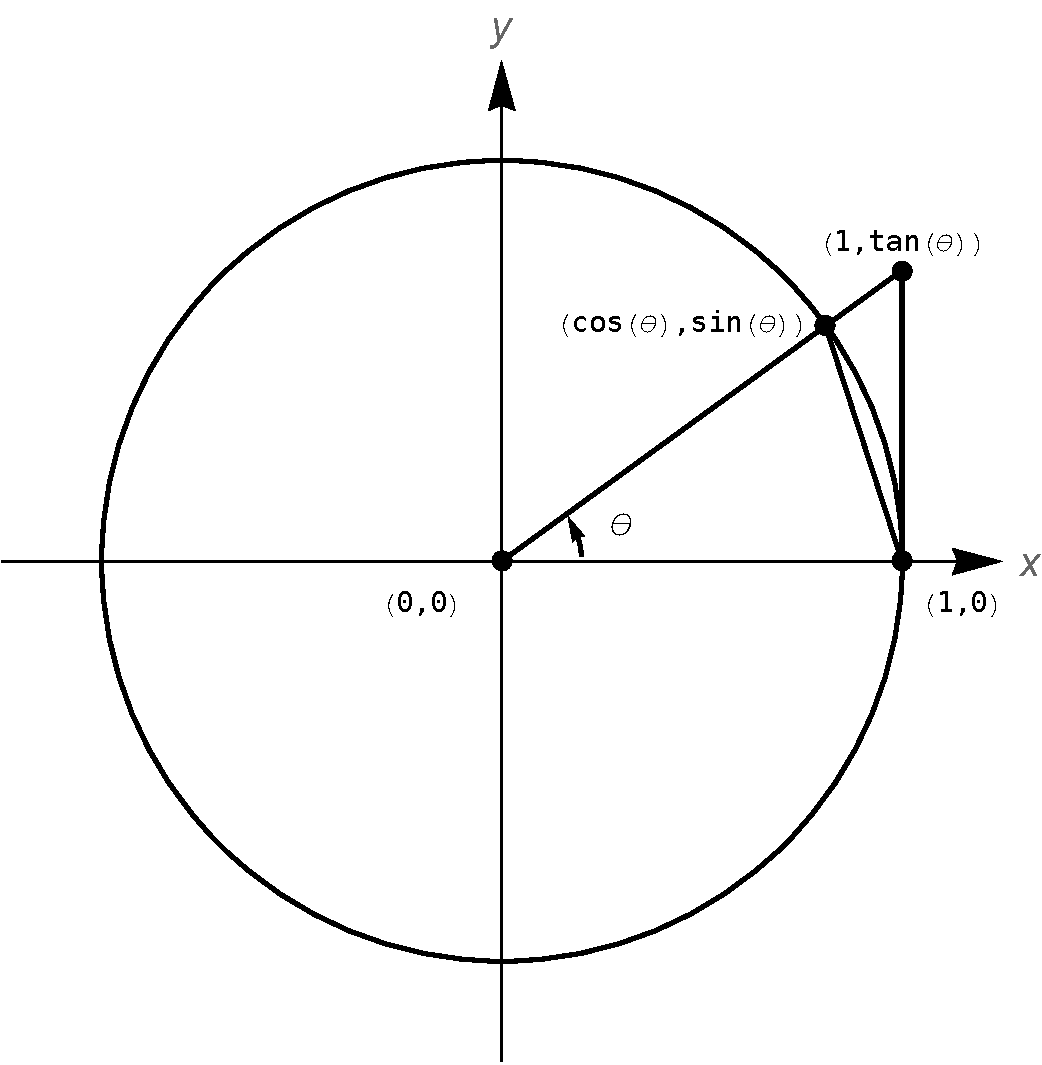
\includegraphics[width=0.5\textwidth]{fig_lim_9}
	\caption{The unit circle and related triangles. }
	\label{fig_lim_9}
	\end{center}
\end{figure}



Figure~\ref{fig_lim_9} shows three regions have been constructed in the first quadrant, two triangles and a sector of a circle, which are also drawn below. The area of the large triangle is $\tan(\theta)/2$; the area of the sector is $\theta/2$; the area of the triangle contained inside the sector is $\sin(\theta)/2$ (Figure~\ref{fig_trans_12}). It is then clear from the diagram that 

\begin{center}
\begin{tabular}{ccccc}
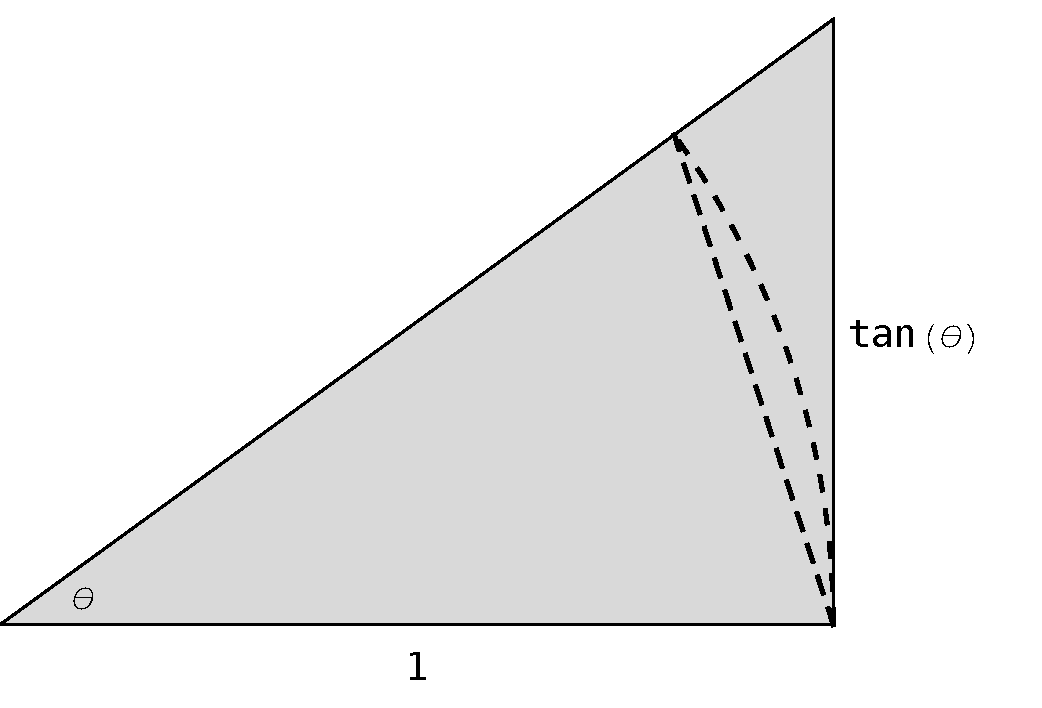
\includegraphics[width=0.3\textwidth]{fig_lim_10a} & & 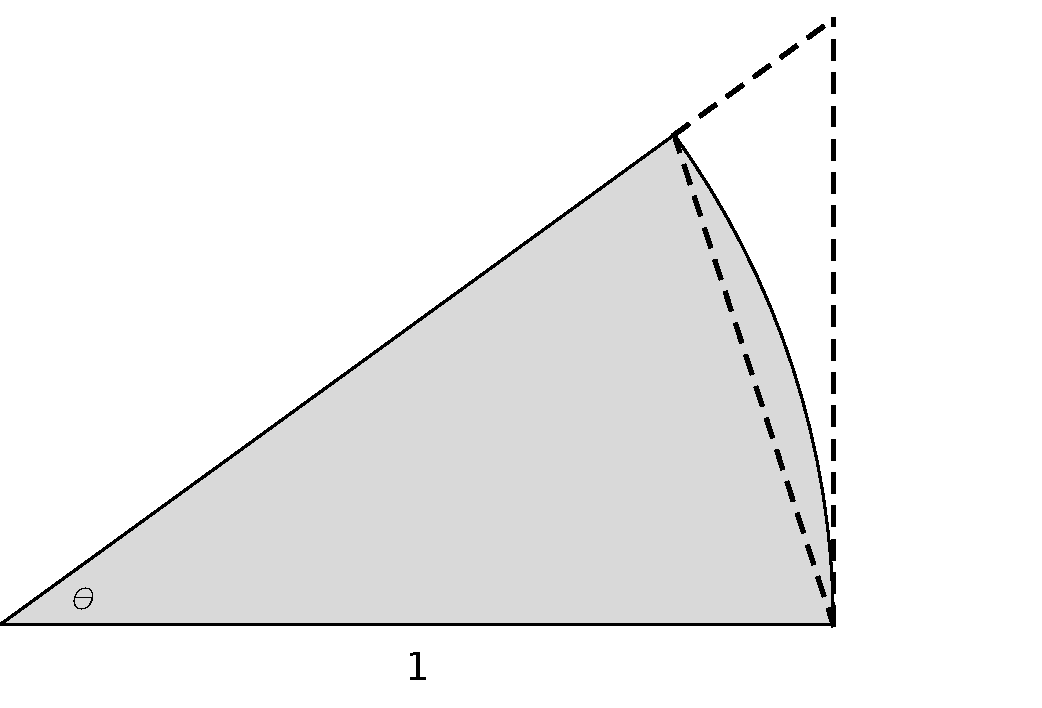
\includegraphics[width=0.3\textwidth]{fig_lim_10b}  & & 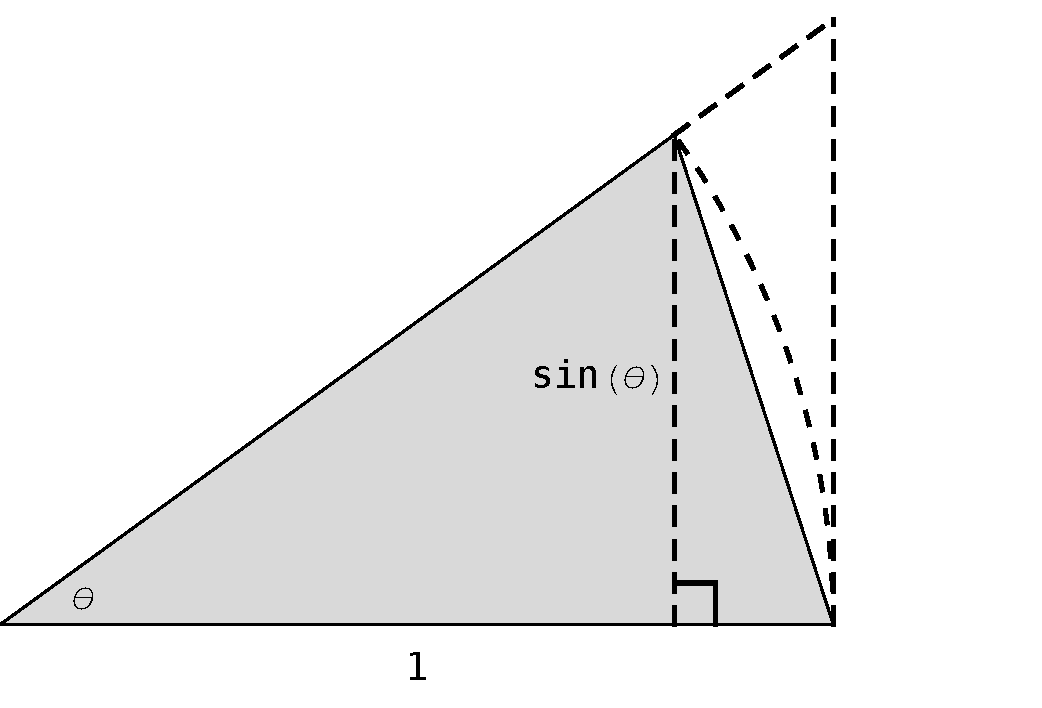
\includegraphics[width=0.3\textwidth]{fig_lim_10c} \\
$\ds \frac{\tan (\theta)}{2}$\rule{0pt}{25pt} & $\geq$ & $\ds \frac{ \theta}{2}$ & $\geq$ & $\ds \frac{\sin  (\theta)}{2}$
\end{tabular}
\end{center}

%$$\frac{\tan(\theta)}{2} \geq \frac{\theta}{2} \geq \frac{\sin (\theta)}{2}.$$

Multiplying all terms in this inequality by $2\sin^{-1} (\theta)$, yields
 $$\frac{1}{\cos(\theta)} \geq \frac{\theta}{\sin (\theta)} \geq 1.$$

Taking reciprocals reverses the inequalities, giving $$ \cos (\theta) \leq \frac{\sin (\theta)}{\theta} \leq 1.$$ Not that these inequalities hold for all values of $\theta$ near 0, even negative values, since \\ $\cos (-\theta) = \cos (\theta)$ and $\sin (-\theta) = -\sin (\theta)$.

Now take limits for $\theta\to 0$.

$$
\begin{array}{rcccl}
\ds\lim_{\theta\to 0} \cos (\theta) &\leq&\ds \lim_{\theta\to 0} \dfrac{\sin(\theta)}{\theta} &\leq&\ds \lim_{\theta\to 0}  1 \\[0.2cm]
\cos (0) &\leq& \ds\lim_{\theta\to 0} \dfrac{\sin(\theta)}{\theta} &\leq&  1 \\[0.2cm]
1&\leq&\ds \lim_{\theta\to 0} \dfrac{\sin(\theta)}{\theta} &\leq&  1
\end{array}
$$

Clearly, Theorem~\ref{thm:sqz} guarantees that 
$$\ds \lim_{\theta\to 0} \frac{\sin(\theta)}{\theta}=1.$$

\end{example}

Actually, this limit tells us more than just that as $x$ approaches 0, $\sin(x)/x$ approaches 1. Both $x$ and $\sin (x)$ are approaching 0, but the ratio of $x$ and $\sin (x)$ approaches 1, meaning that they are approaching 0 in essentially the same way. So for small $x$, the functions $y=x$ and $y=\sin (x)$ are essentially indistinguishable.

We include this special limit, along with three others, which can be determined in a similar way using Theorem~\ref{thm:sqz}, in the following theorem.


\begin{theorem}[Special limits]\label{thm:special_limits}
\noindent\begin{minipage}[t]{.5\textwidth}
\begin{enumerate}
	\item		$\ds \lim_{x\to 0} \frac{\sin (x)}{x} = 1$
	\item		$\ds \lim_{x\to 0} \frac{\cos( x)-1}{x} = 0$
\end{enumerate}
\end{minipage}
\begin{minipage}[t]{.5\textwidth}
\begin{enumerate}\addtocounter{enumi}{2}
	\item		$\ds \lim_{x\to 0} (1+x)^\frac1x = e$
	\item		$\ds \lim_{x\to 0} \frac{e^x-1}{x} = 1$
\end{enumerate}
\end{minipage}
\end{theorem}

A short word on how to interpret the latter three limits in Theorem~\ref{thm:special_limits}. We know that as $x$ goes to 0, $\cos (x)$ goes to 1. So, in the second limit, both the numerator and denominator are approaching 0. However, since the limit is 0, we can interpret this as saying that $\cos (x)$ is approaching 1 faster than $x$ is approaching 0.

In the third limit in Theorem~\ref{thm:special_limits}, inside the parentheses we have an expression that is approaching 1 (though never equalling 1), and we know that 1 raised to any power is still 1. At the same time, the power is growing toward infinity. What happens to a number near 1 raised to a very large power? In this particular case, the result approaches \textbf{Euler's number} (\textit{Eulergetal}), $e$, approximately $2.718.$ Upon an appropriate change of variables, we can also write this as
$$e=\displaystyle\lim_{x\rightarrow \pm\infty} \left( 1+\dfrac{1}{x}\right)^x \,.$$
\index[aut]{Eulergetal} \index{Euler's number}

In the fourth limit in Theorem~\ref{thm:special_limits}, we see that as $x\to 0$, $e^x$ approaches 1 just as fast as $x\to 0$, resulting in a limit of 1.\\

\begin{remark}[Euler's number and interests]
Although the symbol $e$ was introduced by Leonhard Euler around 1727, it was
Jacob Bernoulli who already discovered this constant in 1683 through the third limit in Theorem~\ref{thm:special_limits}. He came across this special limit while studying a question about compound interest:

\textit{A bank account starts with $\$1.00$ and pays 100 percent interest per year. If the interest is credited once, at the end of the year, the value of the account at year-end will be $\$2.00$. What happens if the interest is computed and credited more frequently during the year?}

If there are $n$ compounding intervals, the interest for each interval will be $100\%/n$ and the value at the end of the year will be $\$1.00\,(1 + 1/n)^n$.
\end{remark}
\fi



\subsection{Limits of functions equal at all but one point}
Consider the following limit: 
$$\lim_{x\to 1}\frac{x^2-1}{x-1}.$$

We begin by attempting to apply Theorem \ref{thm:poly_rat} and substituting 1 for $x$ in the quotient. This, however, gives:
		$$\lim_{x\to 1}\frac{x^2-1}{x-1} = \frac{1^2-1}{1-1} = \frac{0}{0},$$ 
an indeterminate form. We cannot apply the theorem.

\begin{figure}
	\begin{center}
			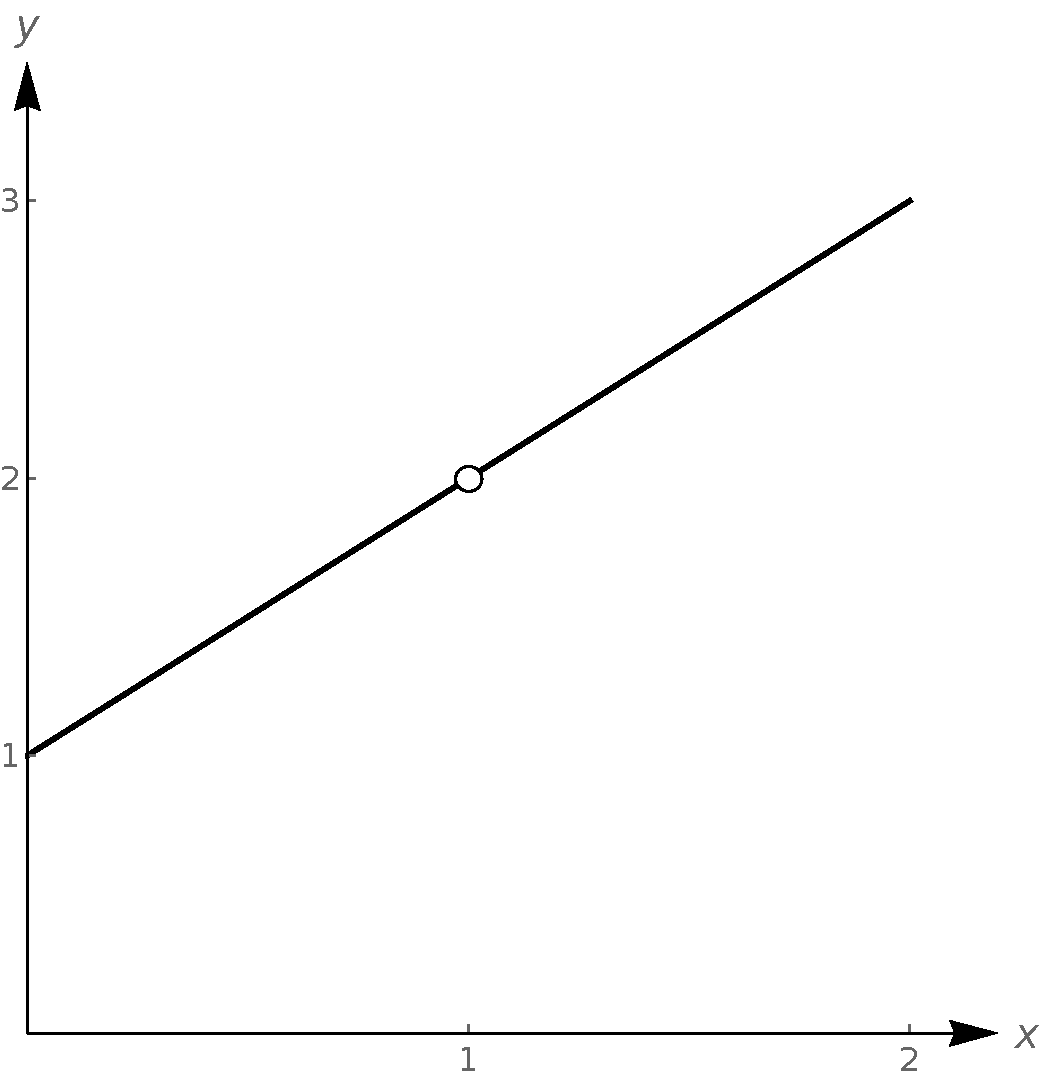
\includegraphics[width=0.4\textwidth]{fig_lim_11}
	\caption{The graph of $y=\frac{x^2-1}{x-1}$. }
	\label{fig_lim_11}
	\end{center}
\end{figure}



By graphing the function $y=\frac{x^2-1}{x-1}$ (Figure~\ref{fig_lim_11}), we see that the function seems to be linear, implying that the limit should be easy to evaluate. Recognize that the numerator of our quotient can be factored:
$$\frac{x^2-1}{x-1} = \frac{(x-1)(x+1)}{x-1}.$$
The function is not defined when $x=1$, but for all other $x$, $$\frac{x^2-1}{x-1} = \frac{(x-1)(x+1)}{x-1} = \frac{\hbox{\sout{$(x-1)$}}(x+1)}{\hbox{\sout{$x-1$}}}= x+1.$$
Clearly $\ds \lim_{x\to 1}(x+1) = 2$. Recall that when considering limits, we are not concerned with the value of the function at 1, only the value the function approaches as $x$ approaches 1. Since $(x^2-1)/(x-1)$ and $x+1$ are the same at all points except $x=1$, they both approach the same value as $x$ approaches 1. Therefore we may conclude that 
$$\lim_{x\to 1}\frac{x^2-1}{x-1}=2.$$


This finding is formalized in the following theorem

\begin{theorem}[Equality of functions and limits]\label{thm:limit_allbut1}
Let $g(x) = f(x)$ for all $x$ in an open interval, except possibly at $c$, and let $\ds \lim_{x\to c} g(x) = L$ for some real number $L$. Then $$\lim_{x\to c}f(x) = L.$$
\end{theorem}

So, when dealing with a rational function of the form $g(x)/f(x)$ and directly evaluating the limit 
$$\ds \lim_{x\to c} \frac{g(x)}{f(x)}$$ 
returns 0/0, the fundamental theorem of algebra tells us that $(x-c)$ is a factor of both $g(x)$ and $f(x)$. One can then use algebra to factor this term out, cancel, and then apply Theorem \ref{thm:limit_allbut1}. 


\ifcourse 
We end this section by revisiting a limit first seen in Section~\ref{sec:limit_intro}, a limit of a difference quotient. Let $f(x) = -1.5x^2+11.5x$; we approximated the limit 
$$\ds \lim_{h\to 0}\frac{f(1+h)-f(1)}{h}\approx 8.5.$$ 

We now formally evaluate this limit in the following example.

\ifanalysis\pagebreak\fi
\begin{example}\label{ex_limit_diffquot}
Let $f(x) = -1.5x^2+11.5x$, then find 
$$\ds \lim_{h\to 0}\frac{f(1+h)-f(1)}{h}.$$

\xhrulefill{gray}{2.5pt}Solution \xhrulefill{gray}{2.5pt}

Since $f$ is a polynomial, our first attempt should be to employ Theorem \ref{thm:poly_rat} and substitute 0 for $h$. However, we see that this gives us $0/0$.

 Knowing that we have a rational function hints that some algebra will help. Consider the following:
		\begin{align*}
		\lim_{h\to 0}\frac{f(1+h)-f(1)}{h} 	&= 	\lim_{h\to 0}\frac{-1.5(1+h)^2 + 11.5(1+h) - \left(-1.5(1)^2+11.5(1)\right)}{h} \\
																				&=	\lim_{h\to 0}\frac{-1.5(1+2h+h^2) + 11.5+11.5h - 10}{h}\\
																				&=	\lim_{h\to 0}\frac{-1.5h^2 +8.5h}{h}\\
																				&= 	\lim_{h\to 0}\frac{h(-1.5h+8.5)}h\\
																				%&=	\lim_{h\to 0}(-1.5h+8.5) \quad \\
																				&= 	8.5. \quad \\
		\end{align*}					
This matches our previous approximation (see Table~\ref{tab_lim_2}).
\end{example}

\fi

This section contains several valuable tools for evaluating limits. One of the main results is that many functions behave in a very nice, predictable way. In Section~\ref{sec:continuity} we give a name to this nice behaviour; we label such functions as continuous. Defining that term will require us to look again at what a limit is and what causes limits to not exist.


For the sake of comprehensiveness, We list below the steps that should be taken when evaluating the limit $\dlim_{x\to a} f(x)$:

\begin{enumerate}
\item Compute $f(a)$.  
\item You arrive at one of the following cases:
\begin{itemize}
\item $ f(a) \in\mathbb{R}$: the limit is computed.  
\item $f(a) = \left(\frac{0}{0}\right)$:  try to get $x-a$ as a common factor in the nominator and denominator, possibly after multiplying with its conjugate binomial, then simplify and return to Step 1.
\item $f(a) = \left(\frac{c}{0}\right) = \pm\infty \, (c \neq 0):\, x=a$ is a vertical asymptote  of the function $f$. 
\end{itemize}
\end{enumerate}


\section{One-sided limits}\label{sec:limit_continuity}

Remember from Section~\ref{sec:limit_intro} that one of the ways in which limits of functions fail to exist is when the function approaches different values from the left and right. To explore in depth the concepts underlying this we introduce in this section  the \textbf{one-sided limit} (\textit{eenzijdige limiet}). We begin with formal definitions that are very similar to Definition~\ref{def:limit}, but the notation is slightly different and $x\neq c$ is replaced with either $x<c$ or $x>c$.

\begin{definition}[One-sided limits]\label{def:onesidedlimit}

\textbf{Left-hand Limit} (\textit{linkerlimiet}) \index{limit ! one sided}\index{limit ! right handed}\index{limit ! left handed}\index[aut]{limiet ! eenzijdig}\index[aut]{limiet ! rechter}\index[aut]{limiet ! linker}\index[aut]{rechterlimiet}\index[aut]{linkerlimiet}

Let $f$ be a function defined on $]a,c[$ for some $a<c$ and let $L$ be a real number. 

The limit of $f(x)$, as $x$ approaches $c$ from the left, is $L$, or, the left-hand limit of $f$ at $c$ is $L$, denoted by  
$$
\displaystyle \lim_{x\underset{<}{\rightarrow}c} f(x) = L,
$$
means  given any $\varepsilon > 0$, there exists $\delta > 0$ such that for all $a<x<c$,  if  $|x - c| < \delta$, then $|f(x) - L| < \varepsilon$.\\



\textbf{Right-hand Limit} (\textit{rechterlimiet})

Let $f$ be a function defined on $]c,b[$ for some $b>c$ and let $L$ be a real number. 

The limit of $f(x)$, as $x$ approaches $c$ from the right, is $L$, or, the right-hand limit of $f$ at $c$ is $L$, denoted by  
$$
\displaystyle \lim_{x\underset{>}{\rightarrow}c} f(x) = L,
$$
means  given any $\varepsilon > 0$, there exists $\delta > 0$ such that for all $c<x<b$,  
if  $|x - c| < \delta$, then $|f(x) - L| < \varepsilon$.
\end{definition}

Practically speaking, when evaluating a left-hand limit, we consider only values of $x$ to the left of $c$, i.e., where $x<c$. The  notation $x\underset{<}{\rightarrow}c$ is used to imply that we look at values of $x$ to the left of $c$.  A similar statement holds for evaluating right-hand limits; there we consider only values of $x$ to the right of $c$, i.e., $x>c$. We can use the theorems from previous sections to help us evaluate these limits; we just restrict our view to one side of $c$.

We practice evaluating left- and right-hand limits through a series of examples.


\begin{example}\label{ex_onesidea}
Let the function $f_1$ be defined by
$$\ds f_1(x) = \left\{\begin{array}{lcl} x, & \mbox{if} & 0\leq x\leq 1, \\ 3-x, & \mbox{if} & 1<x<2.\end{array}\right.$$
Its graph is shown in Figure \ref{fig_lim_12}. Find each of the following: 

\begin{multicols}{4}
	\begin{enumerate}
		\item		$\ds \lim_{x\underset{<}{\rightarrow}1} f_1(x)$
		\item		$\ds \lim_{x\underset{>}{\rightarrow}1} f_1(x)$
		\item		$\ds \lim_{x\to 1} f_1(x)$
		\item		$\ds f_1(1)$
		\item		$\ds \lim_{x\underset{>}{\rightarrow}0} f_1(x)$
		\item		$f_1(0)$
		\item		$\ds \lim_{x\underset{<}{\rightarrow}2} f_1(x)$
		\item		$f_1(2)$
	\end{enumerate}
\end{multicols}

%\noindent\begin{minipage}[t]{.5\textwidth}
%\begin{enumerate}
%\item		$\ds \lim_{x\underset{<}{\rightarrow}1} f_1(x)$
%\item		$\ds \lim_{x\underset{>}{\rightarrow}1} f_1(x)$
%\item		$\ds \lim_{x\to 1} f_1(x)$
%\item		$\ds f_1(1)$
%\end{enumerate}
%\end{minipage}
%\begin{minipage}[t]{.5\textwidth}
%\begin{enumerate}\addtocounter{enumi}{4}
%\item		$\ds \lim_{x\underset{>}{\rightarrow}0} f_1(x)$
%\item		$f_1(0)$
%\item		$\ds \lim_{x\underset{<}{\rightarrow}2} f_1(x)$
%\item		$f_1(2)$
%\end{enumerate}
%\end{minipage}


\begin{figure}[H]
	\begin{center}
			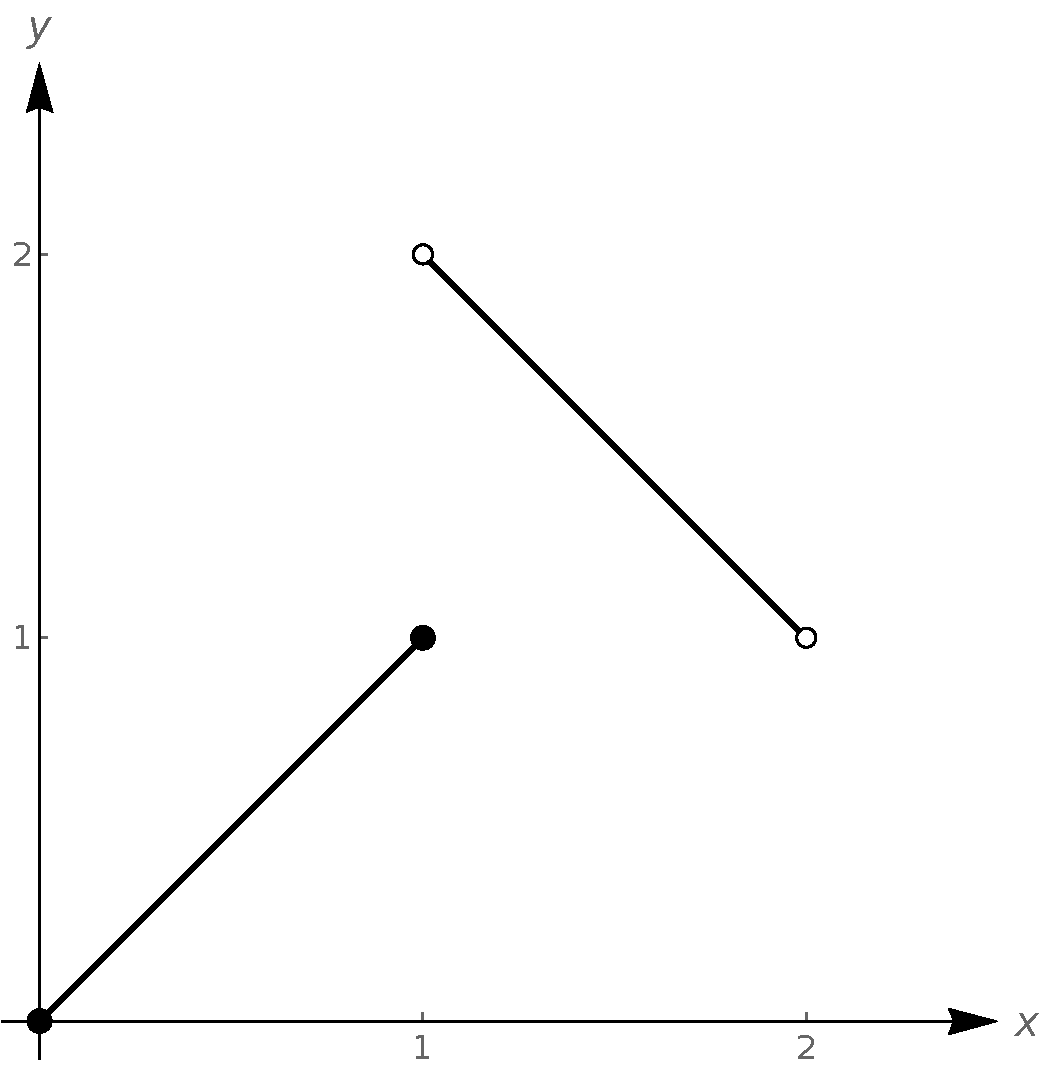
\includegraphics[width=0.3\textwidth]{fig_lim_12}
	\caption{The graph of $f_1$ in Example \ref{ex_onesidea}. }
	\label{fig_lim_12}
	\end{center}
\end{figure}


\xhrulefill{gray}{2.5pt}Solution \xhrulefill{gray}{2.5pt}

For these problems, the visual aid of the graph is likely more effective in evaluating the limits than using $f_1$ itself. 
			\begin{enumerate}
			\item		As $x$ goes to 1 from the left, we see that $f_1(x)$ is approaching the value of 1. Therefore $\ds \lim_{x\underset{<}{\rightarrow}1} f_1(x) =1.$
			\item		As $x$ goes to 1 from the right, we see that $f_1(x)$ is approaching the value of 2. Recall that it does not matter that there is an open circle there; we are evaluating a limit, not the value of the function. Therefore $\ds \lim_{x\underset{>}{\rightarrow}1} f_1(x)=2$.
			\item		The limit of $f_1$ as $x$ approaches 1 does not exist. The function does not approach one particular value, but two different values from the left and the right.
			\item		Using the definition and by looking at the graph we see that $f_1(1) = 1$.
			\item		As $x$ goes to 0 from the right, we see that $f_1(x)$ is also approaching 0. Therefore $\ds \lim_{x\underset{>}{\rightarrow}0} f_1(x)=0$. Note we cannot consider a left-hand limit at 0 as $f_1$ is not defined for values of $x<0$.
			\item		Using the definition and the graph, $f_1(0) = 0$.
			\item\label{lim_onesided_math}		As $x$ goes to 2 from the left, we see that $f_1(x)$ is approaching the value of 1. Therefore $\ds \lim_{x\underset{<}{\rightarrow}2} f_1(x)=1.$
			\item		The graph and the definition of the function show that $f_1(2)$ is not defined.
			\end{enumerate}
\ifmathematica
\ifcourse
Alternatively, we could again make use of Mathematica to determine the one-sided limits. The option \lstinline{Direction} specifies which one-sided limit should be computed ("FromBelow" and "FromAbove" for left-hand and right-hand limits, respectively). For example, we can compute the limit in~\ref{lim_onesided_math} as follows:
\begin{mdframed}[default,backgroundcolor=gray!40,roundcorner=8pt]
\begin{mmaCell}[morefunctionlocal={x},moredefined={Direction}]{Input}
  Limit[Piecewise[\{\{x, 0<=x<=1\}, \{3-x, 1<x<2\}\}], x -> 2, Direction -> "FromBelow"]
\end{mmaCell}

\begin{mmaCell}{Output}
  1
\end{mmaCell}
\end{mdframed}
\fi
\fi

\ifpython
\ifcourse
Alternatively, we could again make use of Python to determine the one-sided limits. The optional fourth argument of  \lstinline{limit} specifies which one-sided limit should be computed ('-' and '+' for left-hand and right-hand limits, respectively). For example, we can compute the limit in~\ref{lim_onesided_math} as follows:
\begin{pyin}
from sympy import limit, symbols
x = symbols('x')
limit(3-x, x, 2, '-')
\end{pyin}
\begin{pyout}
1
\end{pyout}
\fi
\fi
\end{example}

Note how the left and right-hand limits in the previous examples were different at $x=1$. This, of course, causes the limit to not exist. The following theorem states what is fairly intuitive: the limit exists precisely when the left and right-hand limits are equal.

\begin{theorem}[Limits and one sided limits]\label{thm:leftrightlimits}
{Let $f$ be a function defined on an open interval $I$ containing $c$. \index{limit!does not exist} Then $$\lim_{x\to c}f(x) = L$$ if and only if, $$\lim_{x\underset{<}{\rightarrow}c}f(x) = L \quad \text{and} \quad \lim_{x\underset{>}{\rightarrow}c}f(x) = L.$$}
\end{theorem}


Throughout these examples pay attention to the fact that the value of the function may/may not be equal to the value(s) of its left/right-hand limits, even when these limits agree.

\begin{example}\label{ex_onesideb}
Let $$f_2(x) = \left\{\begin{array}{lcl} 2-x, & \mbox{if} &  0<x<1, \\ (x-2)^2, & \mbox{if} &  1<x<2. \end{array}\right.$$ A graph of this function is shown in Figure~\ref{fig_lim_13}. Evaluate the following. 
\begin{multicols}{4}
		\begin{enumerate}
			\item		$\ds \lim_{x\underset{<}{\rightarrow}1} f_2(x)$
			\item		$\ds \lim_{x\underset{>}{\rightarrow}1} f_2(x)$
			\item		$\ds \lim_{x\to 1} f_2(x)$
			\item		$\ds f_2(1)$
			\item		$\ds \lim_{x\underset{>}{\rightarrow}0} f_2(x)$
			\item		$f_2(0)$
			\item		$\ds \lim_{x\underset{<}{\rightarrow}2} f_2(x)$
			\item		$f_2(2)$
		\end{enumerate}	
	\end{multicols}
%\noindent\begin{minipage}[t]{.5\textwidth}
%		\begin{enumerate}
%		\item		$\ds \lim_{x\underset{<}{\rightarrow}1} f_2(x)$
%		\item		$\ds \lim_{x\underset{>}{\rightarrow}1} f_2(x)$
%		\item		$\ds \lim_{x\to 1} f_2(x)$
%		\item		$\ds f_2(1)$
%		\end{enumerate}
%		\end{minipage}
%		\begin{minipage}[t]{.5\textwidth}
%		\begin{enumerate}\addtocounter{enumi}{4}
%		\item		$\ds \lim_{x\underset{>}{\rightarrow}0} f_2(x)$
%		\item		$f_2(0)$
%		\item		$\ds \lim_{x\underset{<}{\rightarrow}2} f_2(x)$
%		\item		$f_2(2)$
%		\end{enumerate}	
%		\end{minipage}
		

\begin{figure}[H]
	\begin{center}
			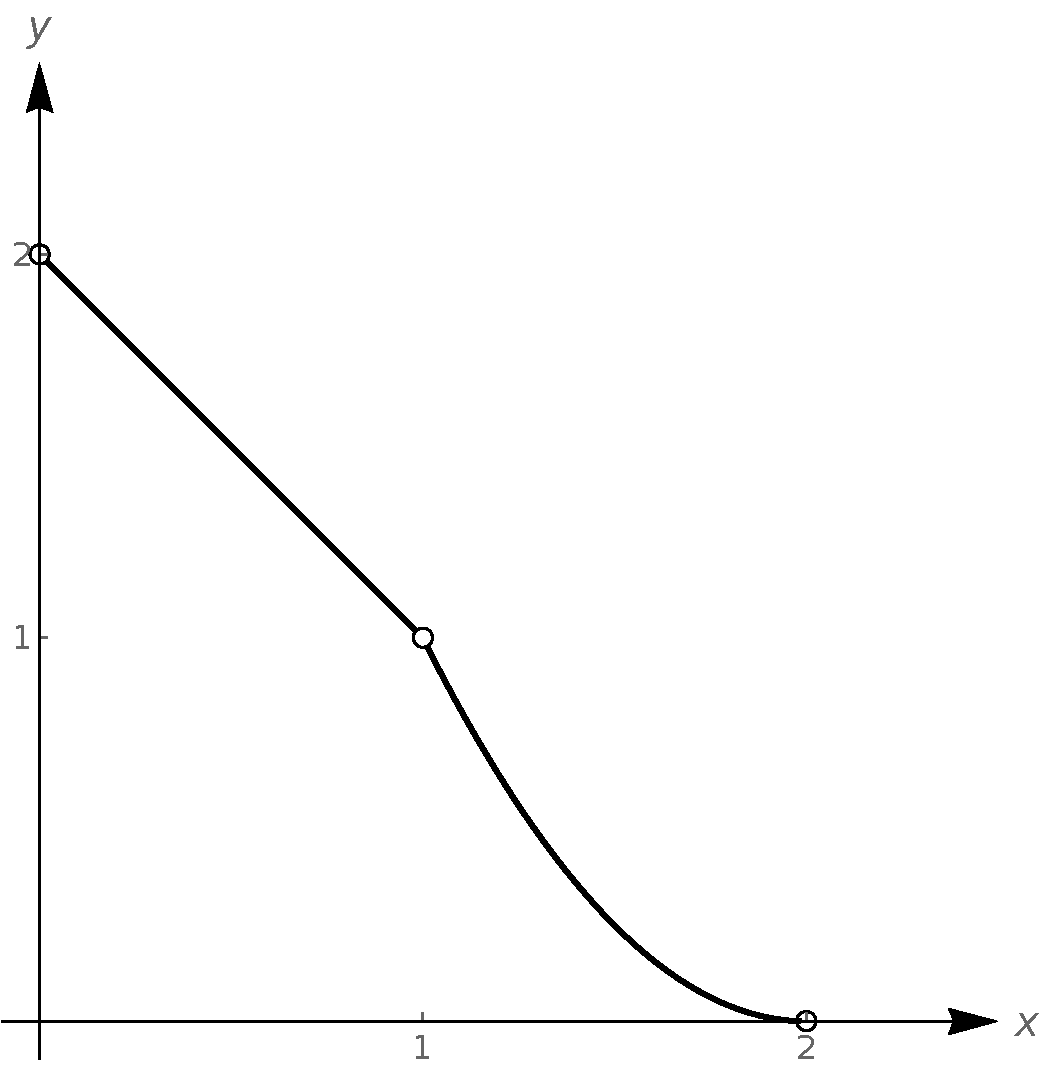
\includegraphics[width=0.3\textwidth]{fig_lim_13}
	\caption{A graph of $f_2$ in Example \ref{ex_onesideb}. }
	\label{fig_lim_13}
	\end{center}
\end{figure}

\xhrulefill{gray}{2.5pt}Solution \xhrulefill{gray}{2.5pt}


We will evaluate each using both the definition of $f_2$ and its graph.
		\begin{enumerate}
		\item		As $x$ approaches 1 from the left, we see that $f_2(x)$ approaches 1. Therefore $\ds \lim_{x\underset{<}{\rightarrow}1} f_2(x)=1.$
		\item		As $x$ approaches 1 from the right, we see that  $f_2(x)$ approaches 1. Therefore $\ds \lim_{x\underset{>}{\rightarrow}1} f_2(x)=1$.
		\item		The limit of $f_2$ as $x$ approaches 1 exists and is 1, as $f_2$ approaches 1 from both the right and left. Therefore $\ds \lim_{x\to 1} f_2(x)=1$.
		\item		$f_2(1)$ is not defined. Note that 1 is not in the domain of $f_2$ as defined by the problem, which is indicated on the graph by an open circle when $x=1$.
		\item		As $x$ goes to 0 from the right, $f_2(x)$ approaches 2. So $\ds \lim_{x\underset{>}{\rightarrow}0} f_2(x)=2$.
		\item		$f_2(0)$  is not defined as $0$ is not in the domain of $f_2$.
		\item		As $x$ goes to 2 from the left, $f_2(x)$ approaches 0. So $\ds \lim_{x\underset{<}{\rightarrow}2} f_2(x)=0$.
		\item		$f_2(2)$  is not defined as 2 is not in the domain of $f_2$.
		\end{enumerate}
\end{example}

\begin{example}
\label{ex_onesidec}
Consider the following piecewise-defined functions:
\begin{multicols}{2}
\begin{enumerate}
\item
$$
f_3(x) = \left\{\begin{array}{lcl} (x-1)^2, & \mbox{if} &  0\leq x\leq 2, x\neq 1, \\ 1, & \mbox{if} &  x=1,\end{array}\right.
$$
\item
$$
f_4(x) = \left\{\begin{array}{lcl} x^2, & \mbox{if} &  0\leq x\leq 1, \\ 2-x, & \mbox{if} &  1<x\leq 2. \end{array}\right.
$$
\end{enumerate}
\end{multicols}
Their graphs are shown  in Figure~\ref{fig_lim_14a} and \ref{fig_lim_14b}, respectively. Evaluate for both functions $\ds \lim_{x\underset{<}{\rightarrow}1} f_i(x)$, $\ds \lim_{x\underset{>}{\rightarrow}1} f_i(x)$, $\ds \lim_{x\to 1} f_i(x)$ and $f_i(1)$.


\begin{figure}[H]
%\raisebox{0.5cm}{
\centerline{
\subfigure[\label{fig_lim_14a}]{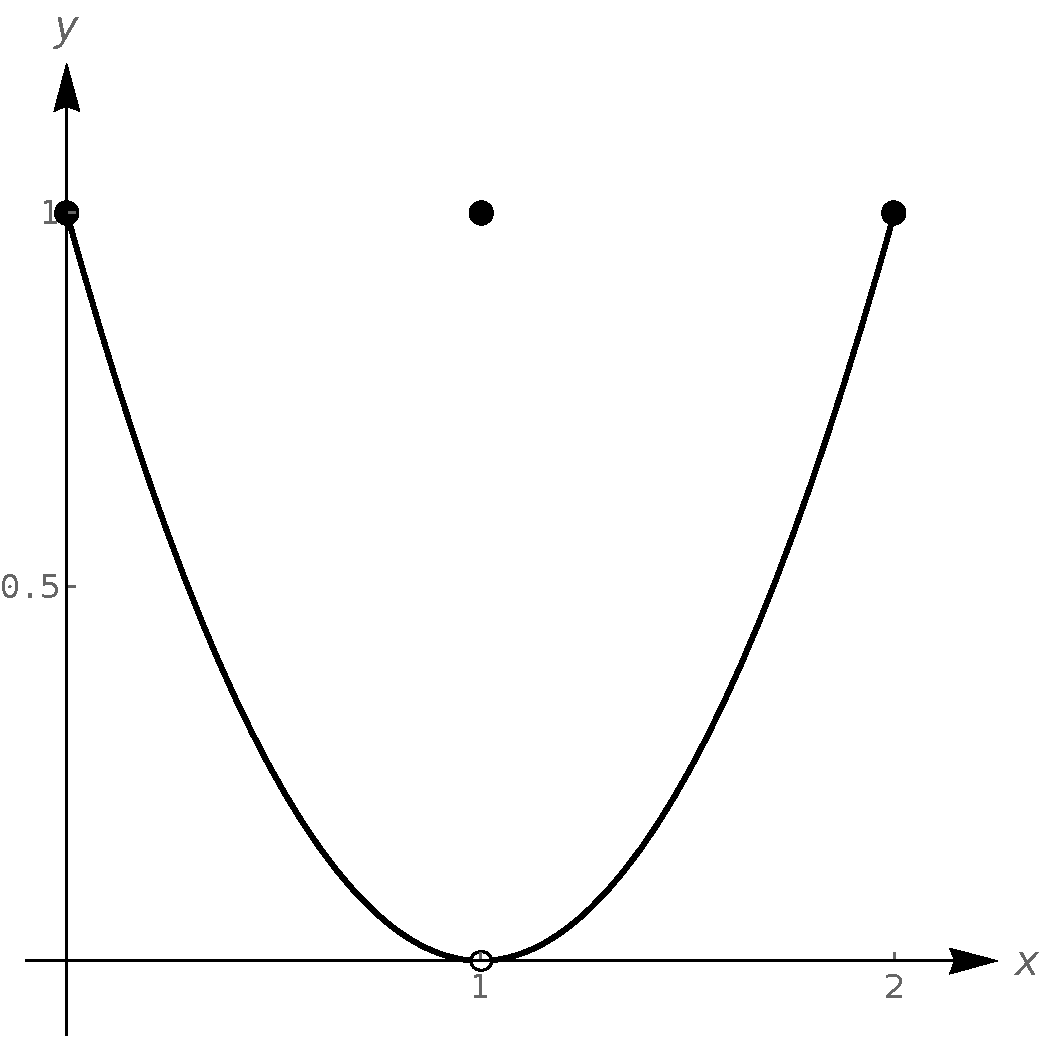
\includegraphics[width=0.3\textwidth]{fig_lim_14a}}
\qquad
\subfigure[\label{fig_lim_14b}]{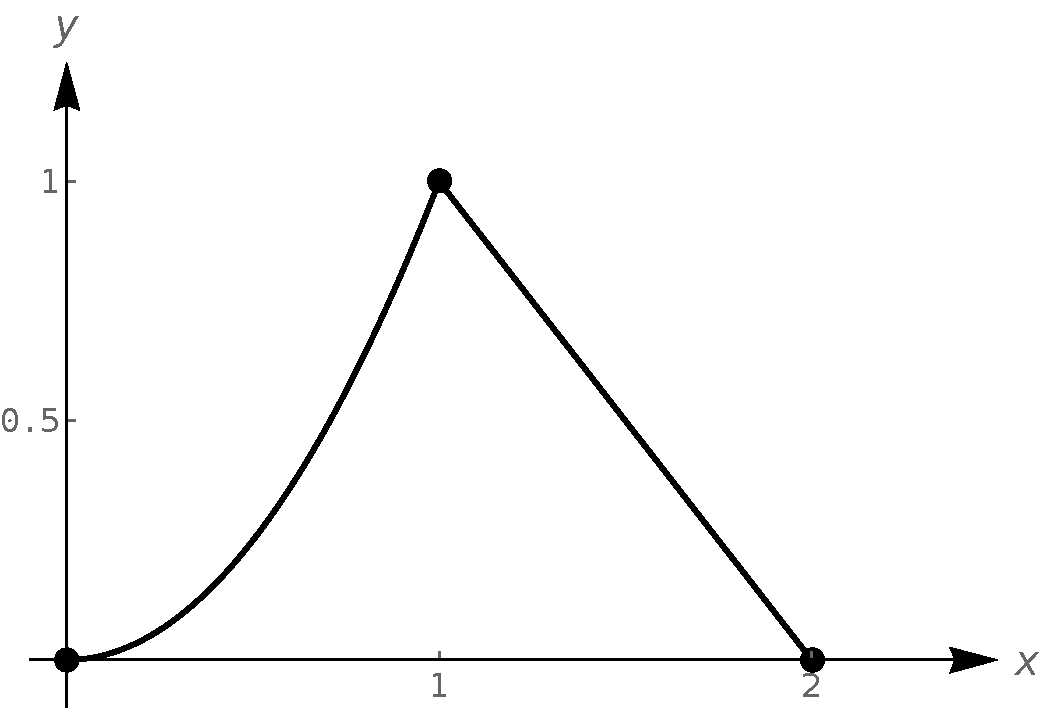
\includegraphics[width=0.3\textwidth]{fig_lim_14b} }
}
\caption{A graph of $f_3$ (a) and $f_4$ (b) in Example \ref{ex_onesidec}. }
\end{figure}



\xhrulefill{gray}{2.5pt}Solution \xhrulefill{gray}{2.5pt}

\begin{enumerate}
\item It is clear by looking at the graph that both the left and right-hand limits of $f_3$, as $x$ approaches 1, are 0. Thus it is also clear that the limit is 0; i.e., $\ds \lim_{x\to 1} f_3(x) = 0$. It is also clearly stated that $f_3(1) = 1$. 
\item It is clear from the definition of the function and its graph that all of the following are equal:
$$ \lim_{x\underset{<}{\rightarrow}1} f_4(x) = \lim_{x\underset{>}{\rightarrow}1} f_4(x) =\lim_{x\to 1} f_4(x) =f_4(1) = 1.$$
\end{enumerate}
\end{example}


In Examples \ref{ex_onesidea} -- \ref{ex_onesidec} we were asked to find both $\ds \lim_{x\to 1}f_i(x)$ and $f_i(1)$. Consider the following table:
\begin{center}
\renewcommand{\arraystretch}{1.5}
\begin{tabular}{c|c|c} & $\ds \lim_{x\to 1}f_i(x)$ & $f_i(1)$ \vspace{2pt}\\ \hline\hline
Example \ref{ex_onesidea} & does not exist & 1 \\
Example \ref{ex_onesideb} & 1 & not defined \\
Example \ref{ex_onesidec}.1 & 0 & 1 \\
Example \ref{ex_onesidec}.2 & 1 & 1 \\
\end{tabular}
\renewcommand{\arraystretch}{1}
\end{center}

Only in Example~\ref{ex_onesidec}.2 do both the function and the limit exist and agree. This seems nice; in fact, it seems normal. This is in fact an important situation which we explore in the next section and refers to a function being continuous. In short, a continuous function is one in which when a function approaches a value as $x\rightarrow c$ (i.e., when $\ds \lim_{x\to c} f(x) = L$), it actually attains that value at $c$. Such functions behave nicely as they are very predictable.



\section{Continuity}\label{sec:continuity}
\subsection{Definition}
As we have studied limits, we have gained the intuition that limits measure where a function is heading. That is, if $\ds \lim_{x\to 1} f(x) = 3$, then as $x$ is close to 1, $f(x)$ is close to 3. We have seen, though, that this is not necessarily a good indicator of what $f(1)$ actually is. This can be problematic; functions can tend to one value but attain another. This section focuses on functions that do not exhibit such behaviour.

\begin{definition}[Continuous function]\label{def:continuous}
Let $f$ be a function defined on an open interval $I$ containing $c$. \index{continuous function} \index[aut]{continue functie}
	\begin{enumerate}
	\item		$f$ is \textbf{continuous} (\textit{continu}) at $c$ if $\ds \lim_{x\to c}f(x) = f(c)$.
	\item		$f$ is continuous on $I$ if $f$ is continuous at $c$ for all values of $c$ in $I$. If $f$ is continuous on $\mathbb{R}$, we say $f$ is continuous everywhere.
	\end{enumerate}
\end{definition}
Note that this definition of continuity (currently) only applies to open intervals.

To establish whether or not a function $f$ is continuous at $c$ one should verify:
		\begin{enumerate}
		\item		$\ds \lim_{x\to c} f(x)$ exists,
		\item		$f(c)$ is defined, and 
		\item		$\ds \lim_{x\to c} f(x) = f(c)$.
		\end{enumerate}
		
		



\begin{example}\label{ex_contint1}
Let $f$ (a) and $g$ (b) be defined as shown in Figures~\ref{fig_lim_15a} and \ref{fig_lim_15b}, respectively. Give the interval(s) on which these functions are continuous.


\begin{figure}[H]
%\raisebox{0.5cm}{
\centerline{
\subfigure[\label{fig_lim_15a}]{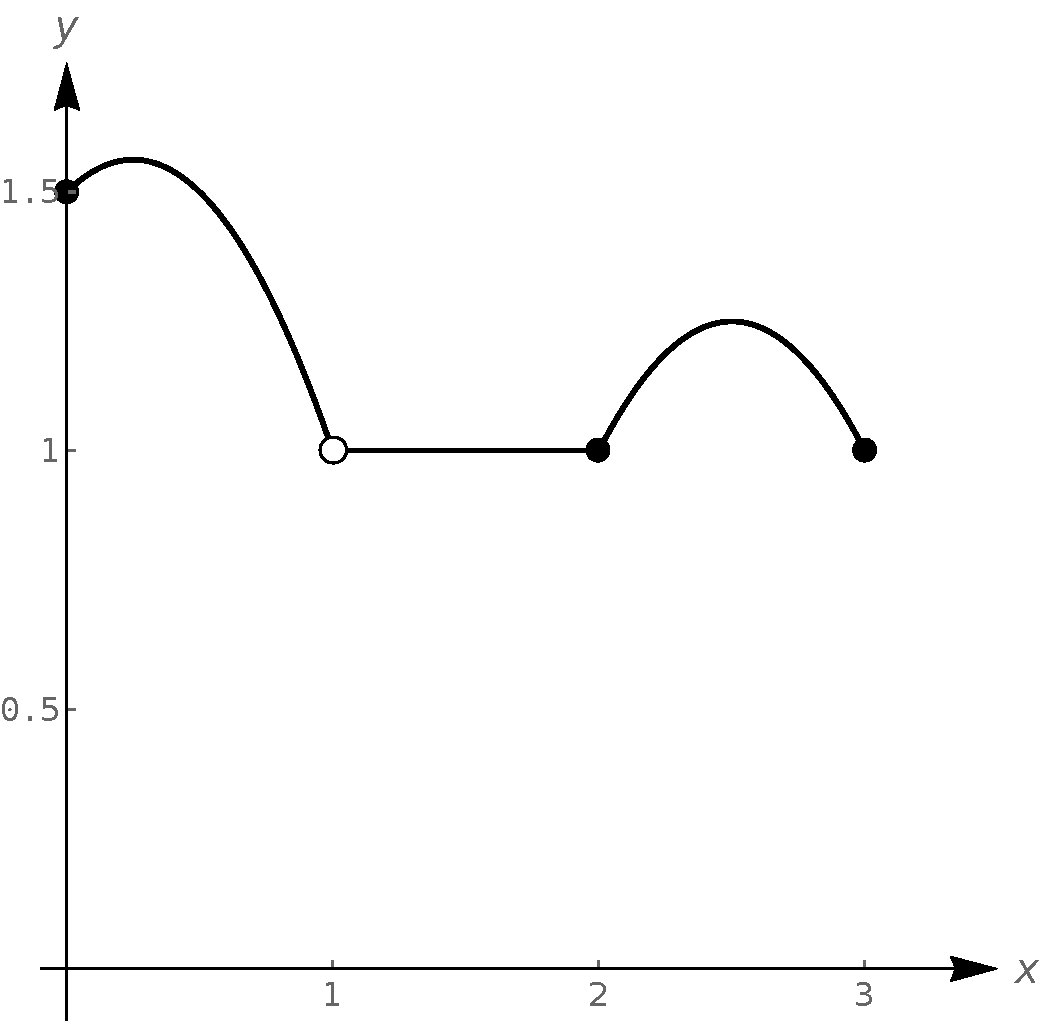
\includegraphics[width=0.3\textwidth]{fig_lim_15a}}
\qquad
\subfigure[\label{fig_lim_15b}]{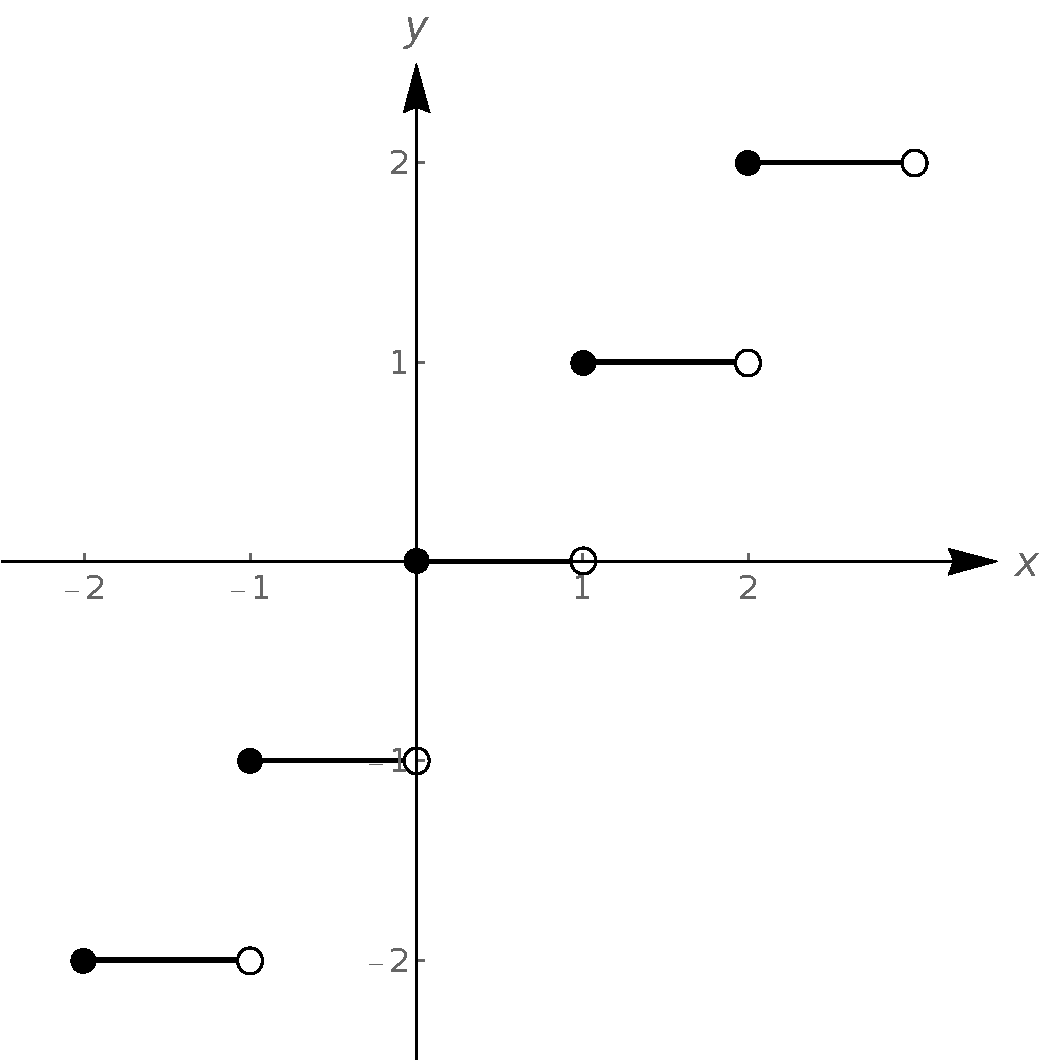
\includegraphics[width=0.3\textwidth]{fig_lim_15b} }
}
\caption{The graph of $f$ (a) and $g$ (b) in Example \ref{ex_contint1}. }
\end{figure}




\xhrulefill{gray}{2.5pt}Solution \xhrulefill{gray}{2.5pt}

\begin{enumerate}
\item [a.] We proceed by examining the three criteria for continuity.
	\begin{enumerate}
	\item		The limits $\ds \lim_{x\to c} f(x)$ exists for all $c$ between 0 and 3.
	\item		$f(c)$ is defined for all $c$ between 0 and 3, except for $c=1$. We know immediately that $f$ cannot be continuous at $x=1$.
	\item		The limit $\ds \lim_{x\to c} f(x) = f(c)$ for all $c$ between 0 and 3, except, of course, for $c=1$. 
	\end{enumerate}

We conclude that $f$ is continuous at every point of $]0,3[$ except at $x=1$. Therefore $f$ is continuous on $\left.\right]0,1\left[\right.$ and $\left.\right]1,3\left[\right.$.
\item [b.] We examine the three criteria for continuity.
		\begin{enumerate}
		\item		The limits $\lim\limits_{x\to c} g(x)$ do not exist at the jumps from one step to the next, which occur at all integer values of $c$. Therefore the limits exist for all $c$ except when $c$ is an integer.
		\item		The function is defined for all values of $c$.
		\item		The limit $\ds \lim_{x\to c} g(x) = g(c)$ for all values of $c$ where the limit exist, since each step consists of just a line. 
		\end{enumerate}
		We conclude that $g$ is continuous everywhere except at integer values of $c$. So the intervals on which $g$ is continuous are $$\ldots, ]-2,-1[, ]-1,0[, ]0,1[, ]1,2[, \ldots\,.$$
		\end{enumerate}
\end{example}

Our definition of continuity on an interval specifies the interval is an open interval. We can extend the definition of continuity to closed intervals by considering the appropriate one-sided limits at the endpoints.

\begin{definition}[Continuity on closed intervals]\label{def:closed_continuity}
Let $f$ be defined on the closed interval $[a,b]$ for some real numbers $a<b$. $f$ is continuous on $[a,b]$ if:
		\begin{enumerate}
		\item		$f$ is continuous on $\left.\right]a,b\left[\right.$,
		\item		$\ds \lim_{x\underset{>}{\rightarrow}a} f(x) = f(a)$ and 
		\item		$\ds \lim_{x\underset{<}{\rightarrow}b} f(x) = f(b)$.
		\end{enumerate}
\end{definition}	
		
We can of course make the appropriate adjustments to talk about continuity on half--open intervals such as $[a,b\left[\right.$ or $\left.\right]a,b]$ if necessary. Also note that we call the function $f$ \textbf{right-continuous} (\textit{rechtscontinu}) at $a$ if
$$\ds \lim_{x\underset{>}{\rightarrow}a} f(x) = f(a)\,,$$
and \textbf{left-continuous} (\textit{linkscontinu}) at $b$ if
$$\ds \lim_{x\underset{<}{\rightarrow}b} f(x) = f(b)\,,$$
where we of course assumed that the respective one-sided limits exist. 
\index{right-continuous}\index{left-continuous}\index[aut]{rechtscontinu}\index[aut]{linkscontinu}

Using this new definition, we can adjust our answer in Example \ref{ex_contint1} by stating that $f$ is continuous on $[0,1\left[\right.$ and $\left.\right]1,3]$. Likewise, the function $g$ in Example \ref{ex_contint1}  is continuous on the following half--open intervals 
$$\ldots, [-2,-1\left[\right., [-1,0\left[\right., [0,1\left[\right., [1,2\left[\right., \ldots.$$

\ifcourse
\ifanalysis

Moreover, bearing in mind Theorem~\ref{thm_lim_bound}, which guarantees that a function is bounded in a $\delta$ neighbourhood of $c$ if the limit at $c$ exists, the next theorem should not come as a surprise. 

\begin{theorem}[Continuity and boundedness of a function]
Let $f$ be continuous on the closed interval $[a,b]$, then $f$ is bounded on $[a,b]$. 
\label{thm_lim_fun_bound}
\end{theorem}

\fi
\fi


Most of the functions you have likely seen in the past are continuous on their domains. This is demonstrated in the following example where we examine the intervals of continuity of a variety of common functions.


\begin{example}\label{ex_cont_funct1}
For each of the following functions, give the domain of the function and the interval(s) on which it is continuous.

\noindent%
\noindent\begin{minipage}[t]{.5\textwidth}
			\begin{enumerate}
				\item		$f(x) = \dfrac{1}{x}$
				\item		$f(x) = \sqrt{x}$
			\end{enumerate}
			\end{minipage}
\begin{minipage}[t]{.5\textwidth}
			\begin{enumerate}\addtocounter{enumi}{2}
				\item		$f(x) = \sqrt{1-x^2}$
				\ifcourse \item		$f(x) = |x|$     \fi
			\end{enumerate}
\end{minipage}

\xhrulefill{gray}{2.5pt}Solution \xhrulefill{gray}{2.5pt}

We examine each in turn.	
		\begin{enumerate}
			\item		The domain of $f(x) = 1/x$ is $\mathbb{R}_0$. As it is a rational function, we apply Theorem \ref{thm:poly_rat} together with Definition~\ref{def:continuous} to recognize that $f$ is continuous on all of its domain.
			\item		The domain of $f(x) = \sqrt{x}$ is $\mathbb{R}^+$. It follows that $f(x) = \sqrt{x}$ is continuous on its domain of $\mathbb{R}^+$.
			\item		The domain of $f(x) = \sqrt{1-x^2}$ is $[-1,1]$. Using properties of limits shows that $f$ is continuous on all of its domain, $[-1,1]$.
			\ifcourse \item		The domain of $f(x) = |x|$ is $\mathbb{R}$. We can define the absolute value function as $$\ds f(x) = \left\{\begin{array}{rcl} -x, & \mbox{if} &  x<0, \\ x, & \mbox{if} &  x\geq 0. \end{array}\right.$$ 
			Each piece of this piecewise defined function is continuous on all of its domain, giving that $f$ is continuous on $\left.\right]-\infty,0\left[\right.$ and $[0,+\infty\left[\right.$. We cannot assume this implies that $f$ is continuous on $\mathbb{R}$; we need to check that $\ds \lim_{x\to 0}f(x) = f(0)$, as $x=0$ is the point where $f$ transitions from one piece of its definition to the other. It is easy to verify that this is indeed true, hence we conclude that $f(x) = |x|$ is continuous everywhere.\fi
		\end{enumerate}
		\end{example}
		
\ifcourse		
\ifanalysis

The continuity of the function $f(x)=|x|$ demonstrated in the previous example is nothing but an illustration of the following theorem.

\begin{theorem}[Continuity of absolute value functions]
Let $f$ be continuous on an interval $I$, then also the function $|f|$, defined as $y= \left|f(x)\right|$, where $x \in I$, is continuous on $I$.
\end{theorem}

\fi
\fi
		
Continuous functions can be combined to form other continuous functions, which is an immediate consequence of the properties of limits. 
So, if we let $f$ and $g$ be continuous functions on an interval $I$,  $c$ be a real number and  $n$ be a positive integer, then the  following functions are continuous on $I$.
		\begin{enumerate}
		\item		\parbox{120pt}{\textbf{Sums/Differences}:}	$f\pm g$
		\item		\parbox{120pt}{\textbf{Constant Multiples}:}	$c\cdot f$
		\item		\parbox{120pt}{\textbf{Products}:}	$f\cdot g$
		\item		\parbox{120pt}{\textbf{Quotients}:}	$f/g$ \qquad {(As long as $g\neq 0$ on $I$.)}
		\item		\parbox{120pt}{\textbf{Powers}:}	$f\,^n$
		\item		\parbox{120pt}{\textbf{Roots}:}	$\sqrt[n]{f}$ \qquad \parbox[t]{200pt}{(If $n$ is even then require $f(x)\geq 0$ on $I$.)}%; if $n$ is odd, then true for all values of $f$ on $I$.)}
		\end{enumerate}
For what concerns function compositions, we consider a function $f$ which is continuous on $I$,  whose range on $I$ is $J$, and a function $g$ which is continuous on $J$. Then $g\circ f$, i.e., $g(f(x))$, is continuous on $I$.


A function $f$ that is not continuous at $c$ is called \textbf{discontinuous} (\textit{discontinu}) at $c$, i.e.\ there is a \textbf{discontinuity} (\textit{discontinu\"iteit}) at $c$.  \index{discontinuous}\index[aut]{discontinu}
\index{discontinuity} \index[aut]{discointinu\"iteit}

\ifcourse
\ifanalysis

There exist several types of discontinuities.  For a so-called \textbf{removable discontinuity} (\textit{ophefbare discontinu\"iteit}), it holds that 
$$
L^{-}=\lim _{x\underset{<}{\rightarrow}c}f(x)
$$
and 
$$
 L^{+}=\lim _{x\underset{>}{\rightarrow}c}f(x) 
$$
at $c$ both exist, are finite, and are equal, i.e.\ $L = L^- = L^+$, but at the same time that the actual value of $f(c)$ is not equal to $L$. This discontinuity can be removed to make $f$ continuous at $c$, or more precisely, the function
$$
 g(x)=\begin{cases}f(x),&x\neq c\\L,&x=c\end{cases}
$$
is continuous at $x = c$. \index{removable discontinuity}\index[aut]{dicontinu\"iteit ! ophefbaar}\index{discontinuity}\index[aut]{dicontinu\"teit}

In the case a single limit does not exist because the one-sided limits, $L^-$ and $L^+$, exist and are finite, but are not equal, $c$ is called a \textbf{jump discontinuity} (\textit{sprong-discontinu\"iteit}). For this type of discontinuity, the function $f$ may have any value at $c$. Finally, there exists also a so-called \textbf{essential discontinuity} (\textit{essenti\"ele discontinu\"iteit}), for which it holds that only one of the two one-sided limits exists or is  infinite.

\index{jump discontinuity}\index[aut]{dicontinuïteit ! sprong}
\index{essential  discontinuity}\index[aut]{dicontinuïteit ! essentieel}

\begin{example}

Identify and classify the discontinuity occurring for each of the following functions.
\begin{multicols}{2}
\begin{enumerate}
\item $f(x)=\left\{\begin{array}{lcl} x^2-2x+3, & \mbox{if} &  x\leq 1, \\ x, & \mbox{if} &  x>1. \end{array}\right.$
\item $f(x) = \left\{\begin{array}{lcl} (x-1)^2, & \mbox{if} &  0\leq x\leq 2, x\neq 1,\\ 1, & \mbox{if} &  x=1.\end{array}\right.$
\item $f(x)=\left\{\begin{array}{lcl} \dfrac{1}{x}, &  \mbox{if} & x\neq 0, \\ 1, & \mbox{if} &  x=0. \end{array}\right.$
\end{enumerate}
\end{multicols}

\xhrulefill{gray}{2.5pt}Solution \xhrulefill{gray}{2.5pt}


\begin{enumerate}
\item A graph of this function is shown in Figure~\ref{fig_lim_3a}. Using the tools we have introduced in the preceding sections, we infer that  $\lim\limits _{x\underset{<}{\rightarrow}1}f(x)=2$ and $\lim\limits _{x\underset{>}{\rightarrow}1}f(x)=1$. Clearly, the left and right-hand limits of $f$ as $x$ approaches 1 exist, but they are different, so the point $x=1$ has a jump discontinuity for this function. 
\item This is the piecewise-defined function that we already encountered in Example~\ref{ex_onesidec} (Figure~\ref{fig_lim_14a}). From our analysis in that example we have that the discontinuity occurs at $x=1$ and that both the left and right-hand limits of $f$, as $x$ approaches 1, are 0. Thus it is also clear that the limit is 0; i.e., $\ds \lim_{x\to 1} f(x) = 0$. At the same time, it holds  that $f$ has the value $1$ in $x=1$. Consequently, the point $x=1$ is a removable discontinuity, which can be removed by defining
$$
g(x)=\begin{cases}f(x),&x\neq 1\\0,&x=1\end{cases}\,.
$$
\item For this function, we can see that at 0 we have some problem of continuity, so we look at what happens with the continuity of the function at this point. We infer that  $\lim\limits _{x\underset{<}{\rightarrow}0}f(x)=-\infty$ and $\lim\limits_{x\underset{>}{\rightarrow}0}f(x)=\infty$, while $f(0)=1$. Hence, we see ourselves confronted with an essential discontinuity. Note that the function $f(x)=1/x$ does not present an essential discontinuity since the function is continuous. We would have the discontinuity at the point $x=0$, but it does not belong to the domain of the function, so it is not possible to define the discontinuity. 
\end{enumerate}

\end{example}

\fi



\subsection{Intermediate value theorem}\label{subsec:IVT}

A common way of thinking of a continuous function is that its graph can be sketched without lifting your pencil. That is, its graph forms a continuous curve, without holes, breaks or jumps. This pseudo--definition glosses, however, over some of the finer points of continuity. Very strange functions are continuous that one would be hard pressed to actually sketch by hand, an example of this being for instance the Weierstrass function (Figure~\ref{fig_lim_16}). 
\begin{figure}[H]
	\begin{center}
			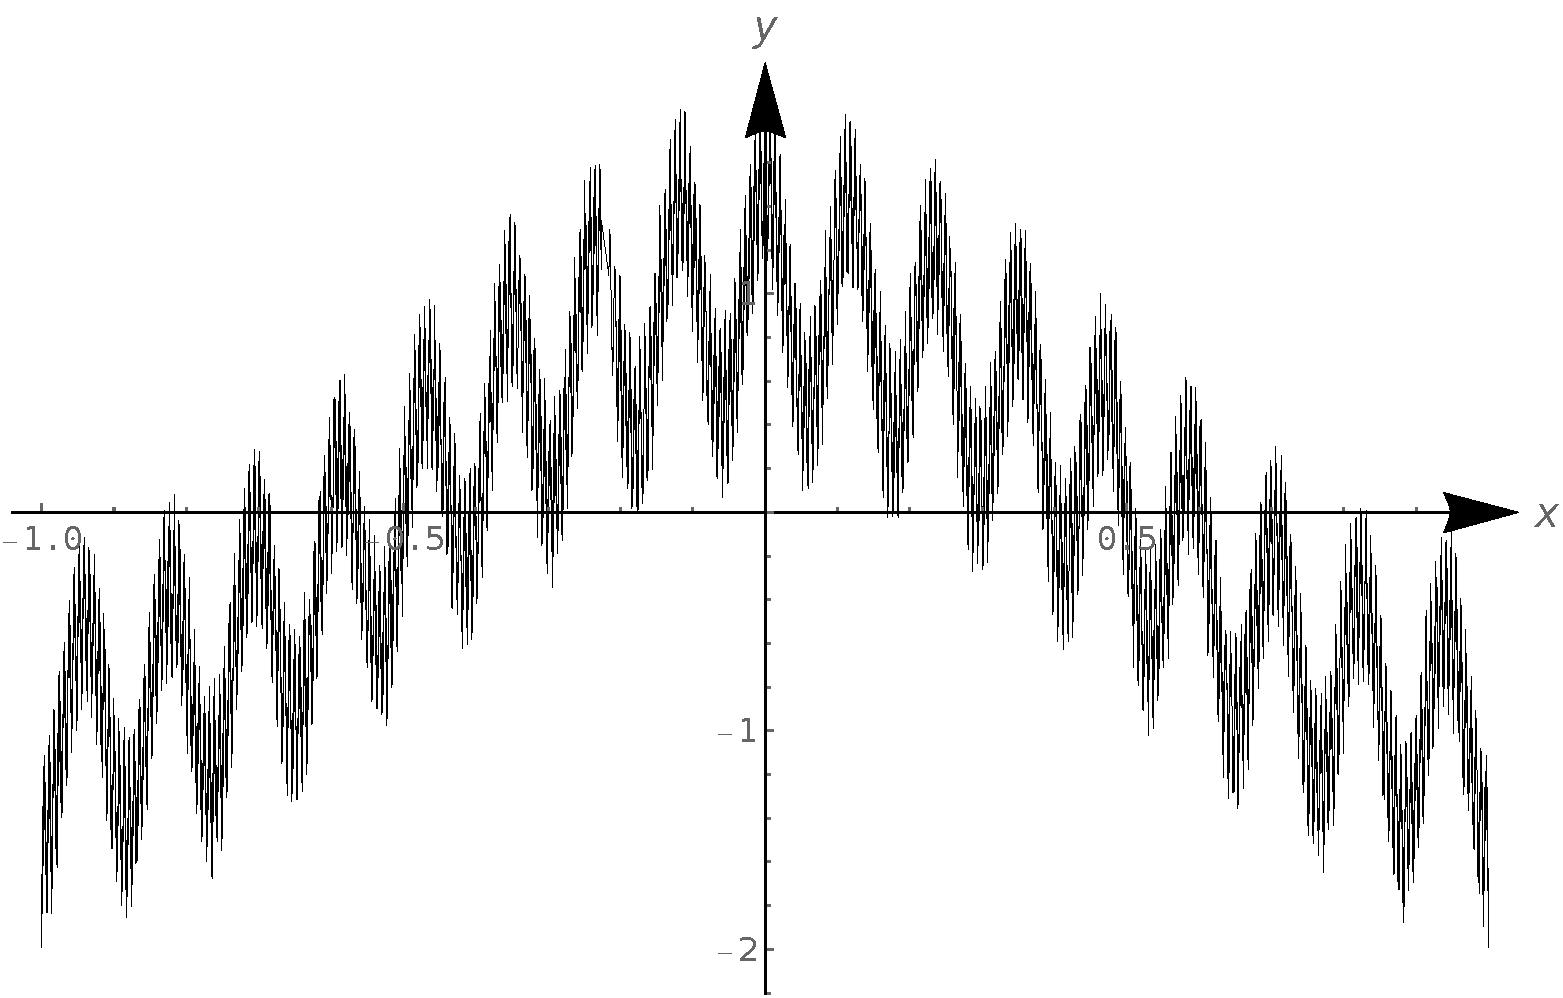
\includegraphics[width=0.45\textwidth]{fig_lim_16}
	\caption{The Weierstrass function.}
	\label{fig_lim_16}
	\end{center}
\end{figure}

	\ifcourse
		\checkoddpage
\marginpar{\ifoddpage\hspace*{-1.5cm}\else\hspace*{0.25cm}\fi
\includegraphics[width=0.075\textwidth]{youtube}\\
\ifoddpage\hspace*{-1.75cm}\else\hspace*{0.1cm}\fi
\qrcode[height=1.75cm]{https://youtu.be/9xgO-EJ3sr0}
%\includegraphics[width=0.1\textwidth]{tussenwaardestelling}
}
 \fi
This intuitive notion of continuity does nonetheless help us understand another important concept as follows. Suppose $f$ is defined on $[1,2]$ and $f(1) = -10$ and $f(2) = 5$. If $f$ is continuous on $[1,2]$ (i.e., its graph can be sketched as a continuous curve from $(1,-10)$ to $(2,5)$) then we know intuitively that somewhere on $[1,2]$ $f$ must be equal to $-9$, and $-8$, and $-7,\ -6,\ \ldots,\ 0,\ 1/2,$ etc. In short, $f$ takes on all intermediate values between $-10$ and $5$. It may take on more values; $f$ may actually equal 6 at some time, for instance, but we are guaranteed all values between $-10$ and 5 will be covered. 

This notion seems intuitive and its importance will turn out to be profound. Therefore the concept is stated in the form of a theorem, the so-called \textbf{intermediate value theorem} (\textit{tussenwaardestelling}).

\begin{theorem}[Intermediate value theorem]\label{thm:IVT}
Let $f$ be a continuous function on $[a,b]$ and, without loss of generality, let $f(a) < f(b)$. Then for every value $u$, where $f(a) < u < f(b)$, there is at least one value $c$ in $\left.\right]a,b\left[\right.$ such that $f(c) = u$. \index{Intermediate value theorem}\index[aut]{Tussenwaardestelling}
\end{theorem}

\ifcalculus
%The intermediate value theorem is illustrated in Figure~\ref{fig_lim_ivt}.


%\begin{figure}
%	\begin{center}
%			\includegraphics[width=0.3\textwidth]{fig_lim_ivta}
%	\caption{Illustration of the intermediate value theorem. }
%	\label{fig_lim_ivt}
%	\end{center}
%\end{figure}


\fi

\ifanalysis

There are several ways to prove the intermediate value theorem, but one way proceeds as follows.

\begin{proof}
Let $S$  be the set of all $ x\in [a,b]$ such that $f (x) \leq u$. Then $S$ is non-empty since $a$ must be an element of $S$. Moreover, $S$ is bounded above by $b$. Hence, by completeness, the supremum $ c=\sup S$ exists. That is, $c$ is the lowest number that is greater than or equal to every member of $S$. We now claim that $f(c) = u$.

Fix some $\varepsilon >0$. Since $f$ is continuous, we have according to Definition~\ref{def:limit} that there is a $\delta >0$ such that $\Big |f(x)-f(c)\Big |<\varepsilon $ whenever $|x-c |< \delta$. This means that
$$
f(x)-\varepsilon<f(c)<f(x)+\varepsilon
$$
on all $ x\in \left.\right]c-\delta ,c+\delta \left[\right.$ (Figure~\ref{fig_lim_17a}). By the properties of the supremum, there exist a  $a^{*}\in \left.\right]c-\delta ,c]$ that is contained in $S$ (Figure~\ref{fig_lim_17b}), so that for that $a^{*}$
$$
f(c)<f(a^{*})+\varepsilon \leq u+\varepsilon\,.
$$
Choose now a $a^{**}\in [c,c+\delta \left[\right.$ that will obviously not be contained in $S$ (Figure~\ref{fig_lim_17c}), so we have
$$
f(c)>f(a^{**})-\varepsilon \geq u-\varepsilon.
$$
Both inequalities
$$
 u-\varepsilon <f(c)<u+\varepsilon
 $$
are valid for all $\varepsilon >0$, from which we deduce $f(c)=u$ as the only possible value, as stated.
\end{proof}

\begin{figure}[h]
%\raisebox{0.5cm}{
\centerline{
\subfigure[\label{fig_lim_17a}]{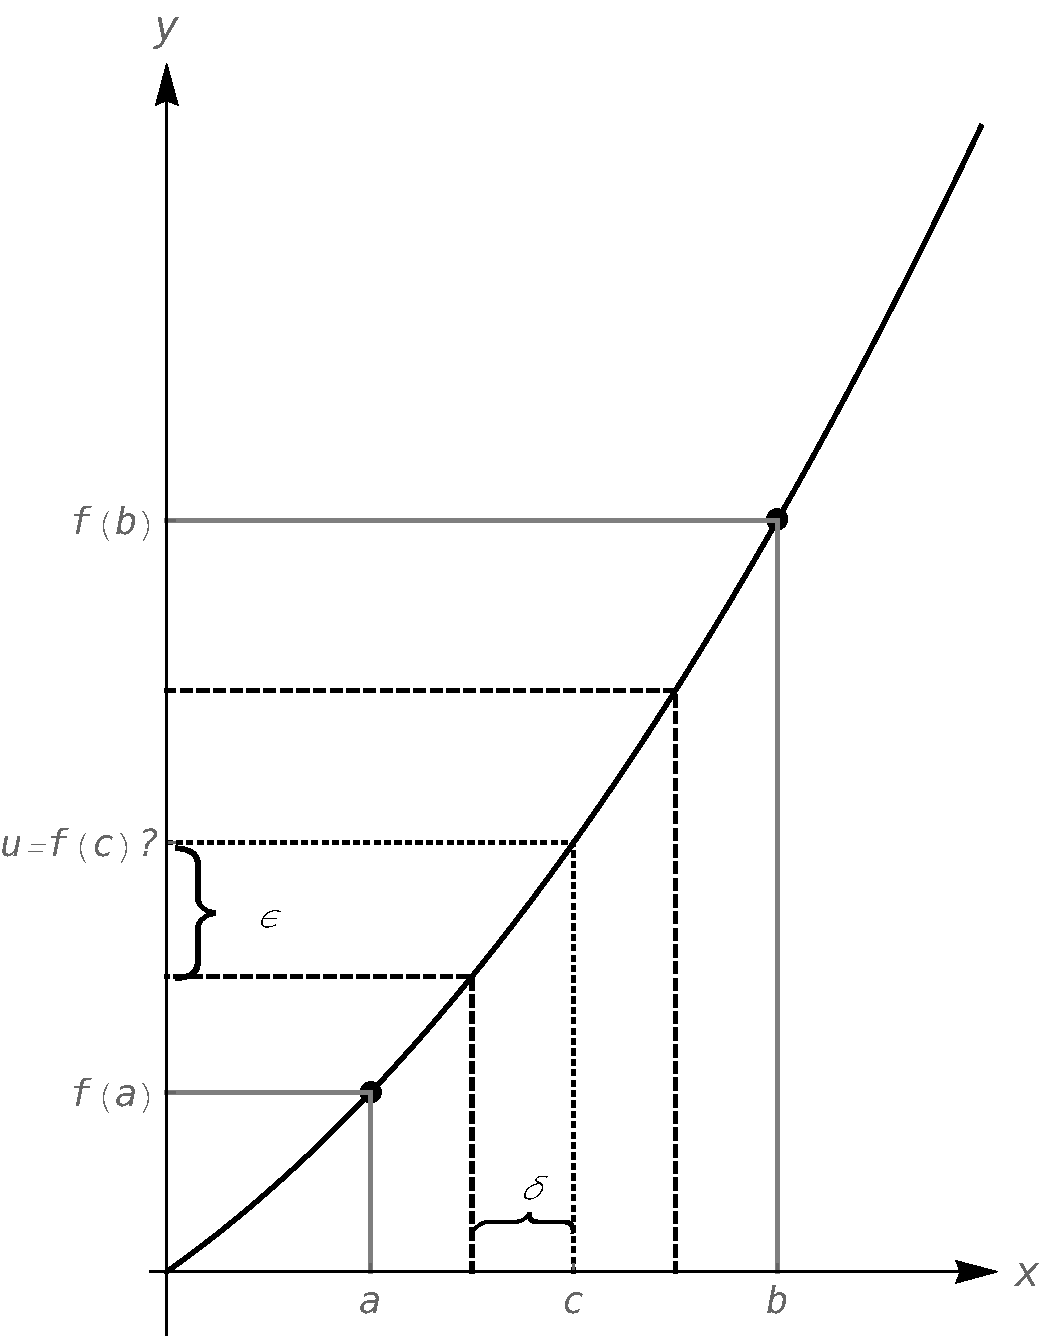
\includegraphics[width=0.3\textwidth]{fig_lim_17a}}
\qquad
\subfigure[\label{fig_lim_17b}]{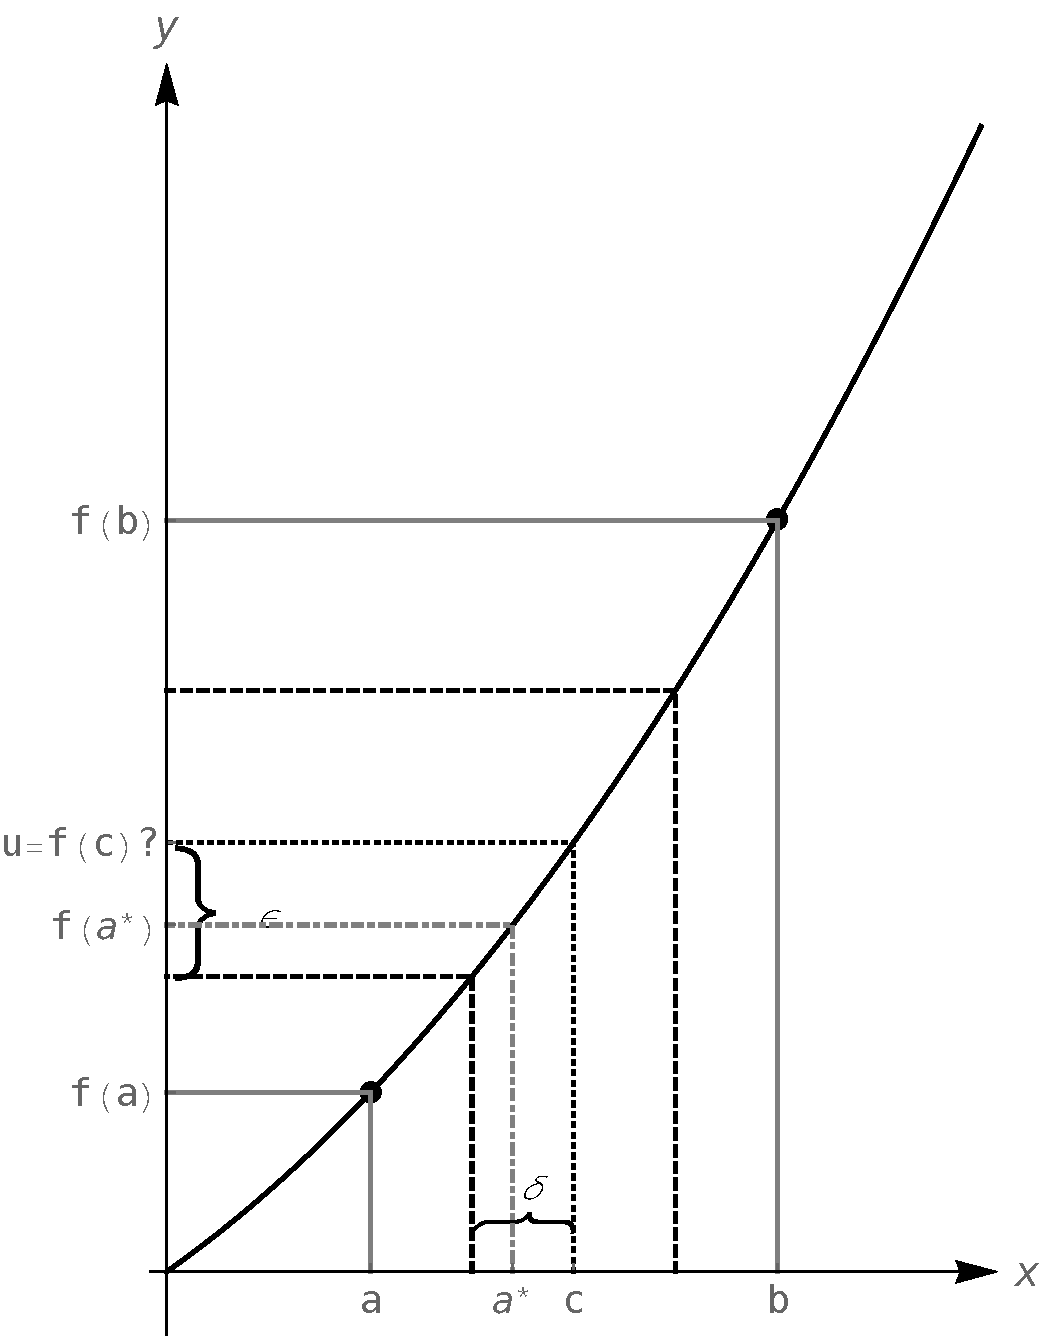
\includegraphics[width=0.3\textwidth]{fig_lim_17b} }
\qquad
\subfigure[\label{fig_lim_17c}]{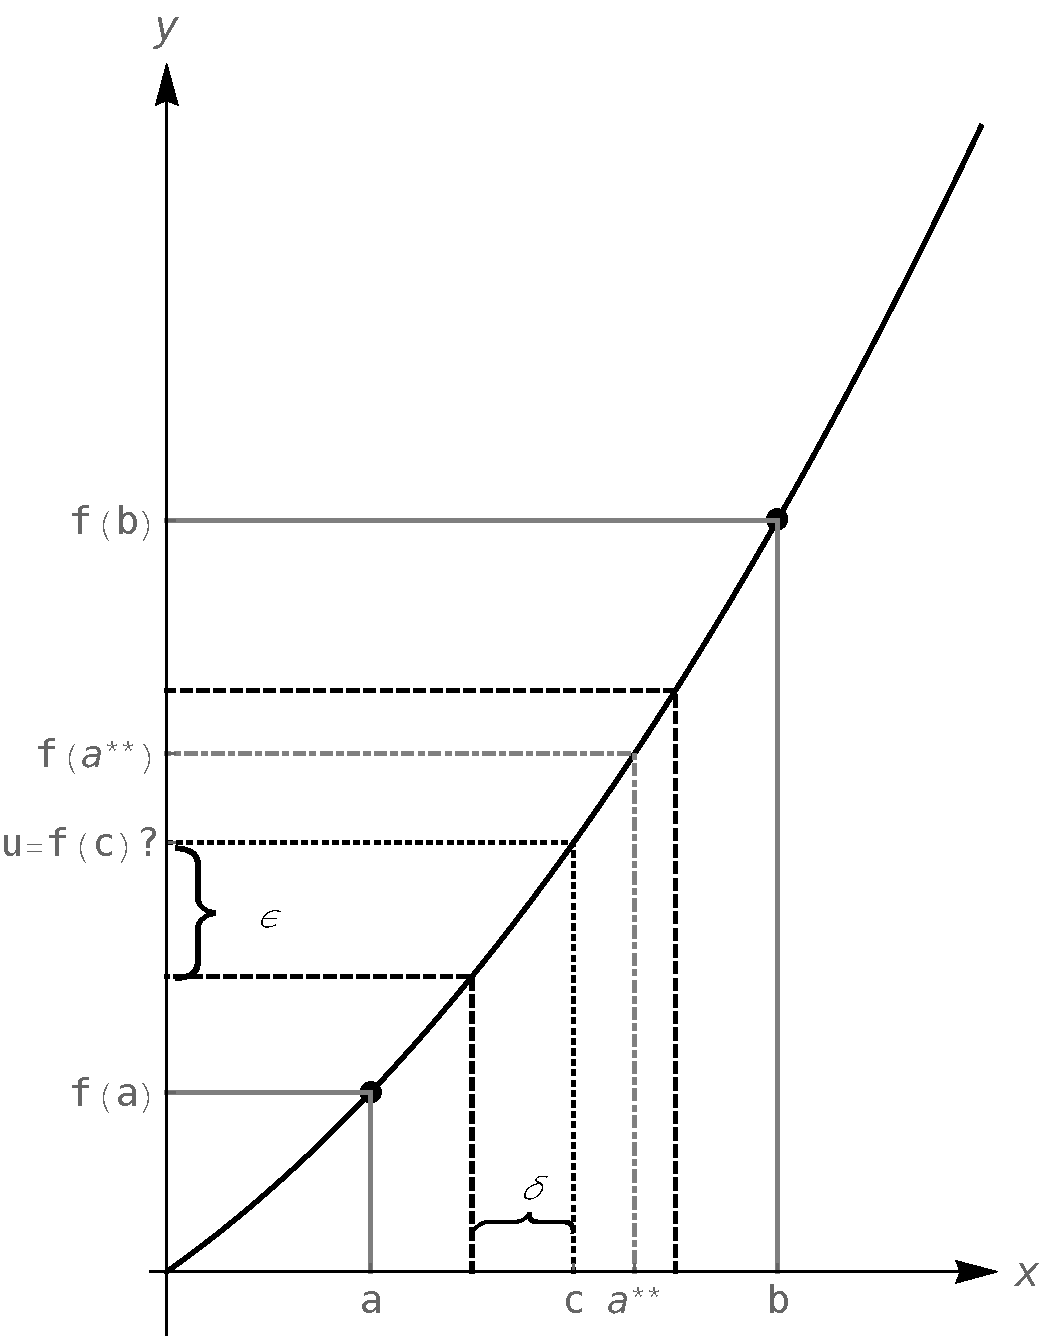
\includegraphics[width=0.3\textwidth]{fig_lim_17c} }
}
\caption{Proving the intermediate value theorem. }
\end{figure}




\fi

One important application of the intermediate value theorem is root finding. Given a function $f$, we are often interested in finding values of $x$ where $f(x) = 0$. These roots may be very difficult to find exactly. Good approximations can be found through successive applications of this theorem. Suppose through direct computation we find that $f(a) <0 $ and $f(b)>0$, where $a<b$. The intermediate value theorem states that there is at least one $c$ in $\left.\right]a,b\left[\right.$ such that $f(c) = 0$. The theorem does not give us any clue as to where to find such a value in the interval $\left.\right]a,b\left[\right.$, just that at least one such value exists. 

There is a technique that produces a good approximation of $c$. Let $d$ be the midpoint of the interval $[a,b]$ and consider $f(d)$. There are three possibilities:
	\begin{enumerate} 
	\item		$f(d) = 0$: We got lucky and stumbled on the actual value. We stop as we found a root.
	\item		$f(d) <0$: Then we know there is a root of $f$ on the interval $[d,b]$ -- we have halved the size of our interval, hence are closer to a good approximation of the root.
	\item		$f(d) >0$: Then we know there is a root of $f$ on the interval $[a,d]$ -- again,we have halved the size of our interval, hence are closer to a good approximation of the root.
	\end{enumerate}

Successively applying this technique is called the \textbf{bisection method} (\textit{halveringsmethode})\index{bisection method}\index[aut]{halveringsmethode} of root finding. We continue until the interval is sufficiently small. We demonstrate this in the following example.

\begin{example}\label{ex_bisect_method}
Approximate the root of $f(x) = x-\cos (x)$, accurate to three places after the decimal.

\xhrulefill{gray}{2.5pt}Solution \xhrulefill{gray}{2.5pt}


Consider the graph of $f(x) = x-\cos (x)$, shown in Figure~\ref{fig_lim_18a}. It is clear that the graph crosses the $x$-axis somewhere near $x=0.8$. To start the bisection method, pick an interval that contains $0.8$. We choose $[0.7,0.9]$. Note that all we care about are signs of $f(x)$, not their actual value, so this is all we display.


		\begin{description}
		\item [Iteration 1:] $f(0.7) < 0$, $f(0.9) > 0$, and $f(0.8) >0$. So replace $0.9$ with $0.8$ and repeat.
		\item	[Iteration 2:]	$f(0.7)<0$, $f(0.8) > 0$, and at the midpoint, $0.75$, we have $f(0.75) >0 $. So replace $0.8$ with $0.75$ and repeat. Note that we do not need to continue to check the endpoints, just the midpoint. Thus we put the rest of the iterations in Table~\ref{fig_lim_18b}.
		\end{description}
		


			
Notice that in the 12$^\text{th}$ iteration we have the endpoints of the interval each starting with $0.739$. Thus we have narrowed the zero down to an accuracy of the first three places after the decimal. Using a computer, we have 
$$ f(0.7390) = -0.00014, \quad f(0.7391) = 0.000024.$$ Either endpoint of the interval gives a good approximation of where $f$ is 0. The intermediate value theorem states that the actual zero is still within this interval. While we do not know its exact value, we know it starts with $0.739$. 

This type of exercise is rarely done by hand. Rather, it is simple to program a computer to run such an algorithm and stop when the endpoints differ by a preset small amount. 
\end{example}

\begin{figure}\ifcalculus[h]\fi
%\raisebox{0.5cm}{
\centerline{
\subfigure[Graph of $f(x) = x-\cos x$ near a root. \label{fig_lim_18a}]{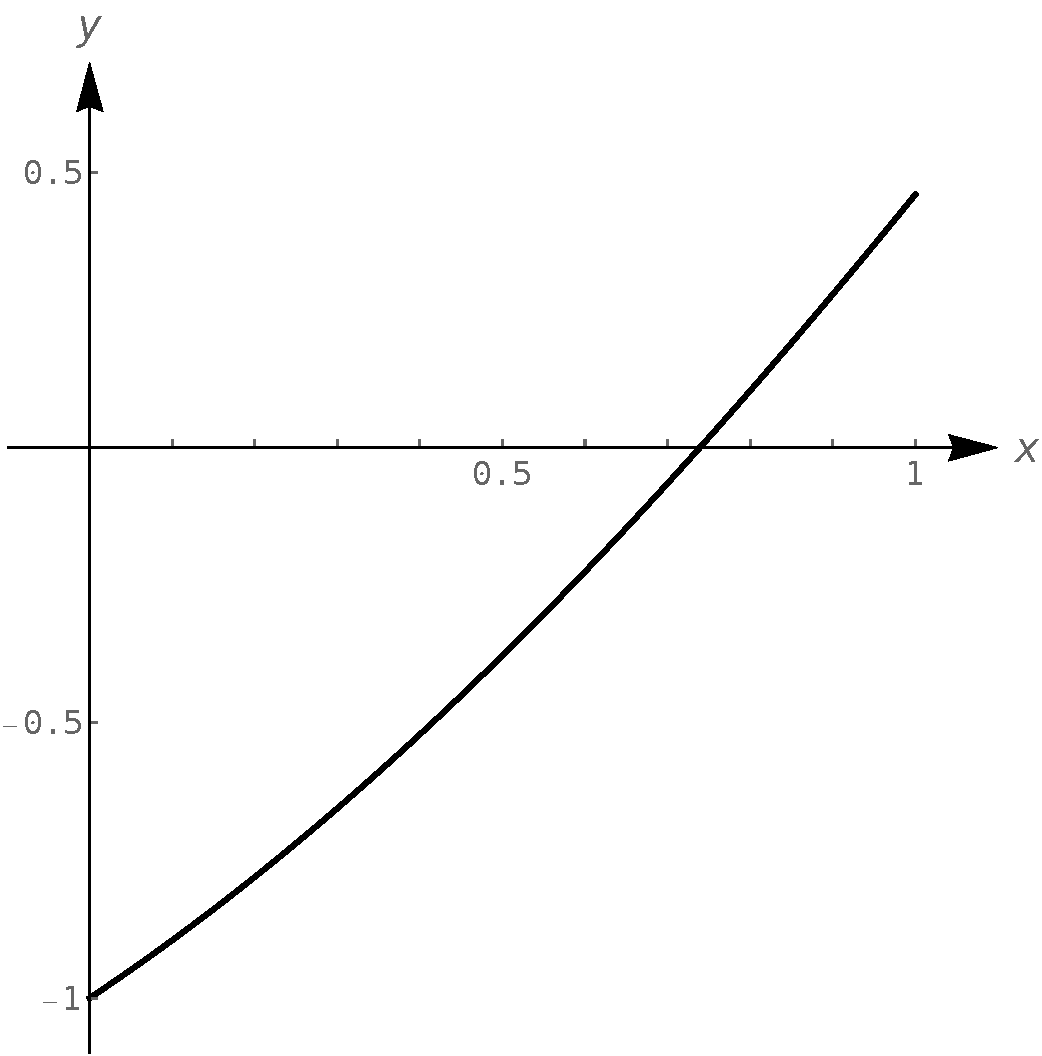
\includegraphics[width=0.45\textwidth]{fig_lim_18a}}
\qquad
\subfigure[\label{fig_lim_18b}]{\renewcommand{\arraystretch}{1.25}\begin{tabular}[b]{c|cc}
			Iteration \# & Interval & Midpoint Sign \\ \hline\hline
			1		& $[0.7,0.9]$ & $f(0.8) >0$ \\
			2 & $[0.7,0.8] $ & $f(0.75) >0$ \\
			3 & $[0.7,0.75]$ & $f(0.725)<0$\\
			4 & $[0.725,0.75]$ & $f(0.7375)<0$\\
			5 & $[0.7375,0.75]$ & $f(0.7438)>0$\\
			6 & $[0.7375,0.7438]$ & $f(0.7407)>0$\\
			7 & $[0.7375,0.7407]$ & $f(0.7391)>0$\\
			8 & $[0.7375,0.7391]$ & $f(0.7383)<0$\\
			9 & $[0.7383,0.7391]$ & $f(0.7387)<0$\\
			10 & $[0.7387,0.7391]$ & $f(0.7389)<0$\\
			11 & $[0.7389,0.7391]$ & $f(0.7390)<0$\\
			12 & $[0.7390,0.7391]$ &   \\
			\end{tabular}
			\renewcommand{\arraystretch}{1}
}}
\caption{Finding a root of $f(x) = x-\cos x$. }
\end{figure}



It is a simple matter to extend the bisection method.  For instance, we can find $x$, where $f(x) = 1$. %This may seem obvious, but to many it is not. 
It actually works very well to define a new function $g$ where $g(x) = f(x) - 1$. Then use the bisection method to solve $g(x)=0$.  Similarly, given two functions $f$ and $g$, we can use this method to solve $f(x) = g(x)$. Once again, create a new function $h$ where $h(x) = f(x)-g(x)$ and solve $h(x) = 0$. 

\fi



\section{Limits involving infinity}\label{sec:limits_infty}

In Definition~\ref{def:limit} we stated that in the equation $\lim\limits_{x\to c}f(x) = L$, both $c$ and $L$ were real numbers. In this section we relax that definition a bit by considering situations when it makes sense to let $c$ and/or $L$ be infinity. Essentially, we allow $c$ and/or $L$ to be in the set of extended real number $\overline{\mathbb{R}}$ (Section~\ref{sec_real}). 

As a motivating example, consider $f(x) = \frac{1}{x^2}$, as shown in Figure~\ref{fig_lim_19}. Note how, as $x$ approaches 0, $f(x)$ grows very, very large -- in fact, it grows without bound. It seems appropriate, and descriptive, to state that $$\lim_{x\rightarrow 0} x^{-2}=+\infty.$$ Also note that as $x$ gets very large, $f(x)$ gets very, very small. We could represent this concept with notation such as $$\lim_{x\rightarrow +\infty} \frac1{x^2}=0.$$


We explore both types of use of infinity in turn.

\begin{figure}[H]
	\begin{center}
			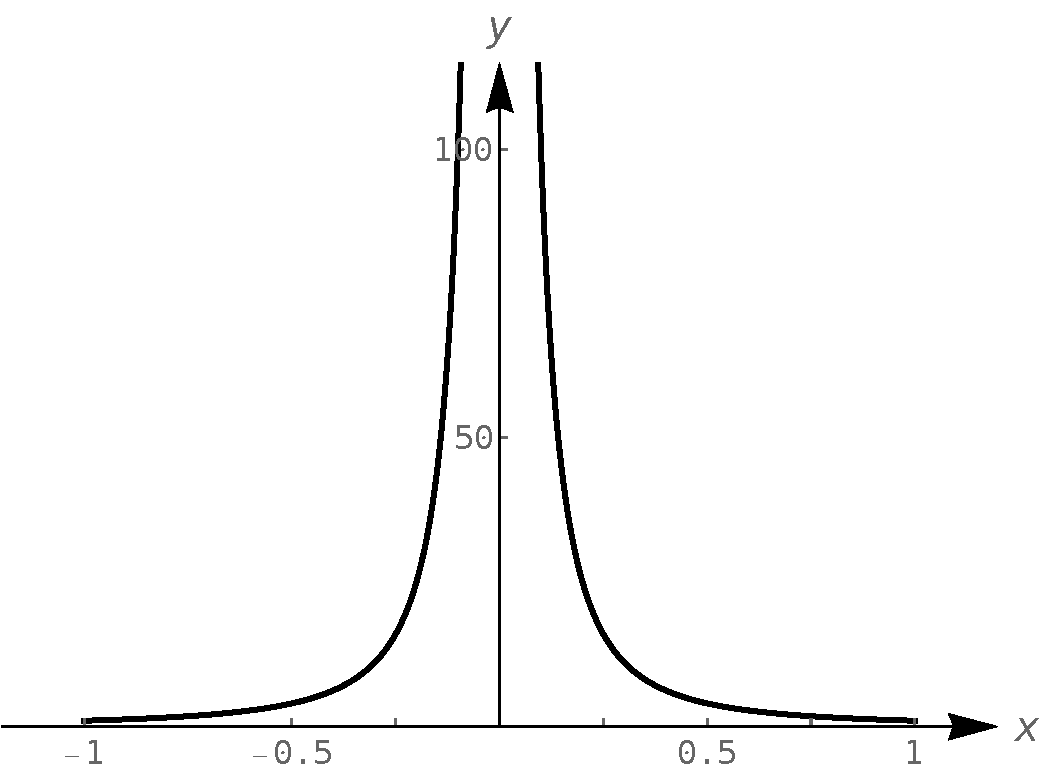
\includegraphics[width=0.4\textwidth]{fig_lim_19}
	\caption{Graphing $f(x) = \frac{1}{x^2}$ for values of $x$ near 0. }
	\label{fig_lim_19}
	\end{center}
\end{figure}


\subsection{Limits of infinity and vertical asymptotes}



\begin{definition}[Limit of infinity]\label{def:limit_of_infinity}
Let $I$ be an open interval containing $c$, and let $f$ be a function defined on $I$, except possibly at $c$. 
\begin{itemize}
\item The limit of $f(x)$, as $x$ approaches $c$, is positive infinity, denoted by  
$$\displaystyle \lim_{x\rightarrow c} f(x) = +\infty,$$
means that given any $N > 0$, there exists $\delta > 0$ such that for all $x$ in $I$, where $x\neq c$,  
if  $|x - c| < \delta$, then $f(x) >N$.

\item The limit of $f(x)$, as $x$ approaches $c$, is negative infinity, denoted by  
$$\displaystyle \lim_{x\rightarrow c} f(x) = -\infty,$$
means that given any $N < 0$, there exists $\delta > 0$ such that for all $x$ in $I$, where $x\neq c$,  
if  $|x - c| < \delta$, then $f(x)  < N$.

\end{itemize}%
\index{limit ! of infinity}
\index[aut]{limiet ! oneigenlijk}
\index[aut]{oneigenlijke limiet}
\end{definition}


\ifcourse

The first definition is similar to the $(\varepsilon,\delta)$-definition  (Definition~\ref{def:limit}).  In that definition, given any (small) value $\varepsilon$, if we let $x$ get close enough to $c$ (within $\delta$ units of $c$) then $f(x)$ is guaranteed to be within $\varepsilon$ of $L$.  Here, given any (large) value $N$, if we let $x$ get close enough to $c$ (within $\delta$ units of $c$), then $f(x)$ will be at least as large as $N$.  In other words, if we get close enough to $c$, then we can make $f(x)$ as large as we want.

\ifanalysis

Of course, we may easily extend the squeeze theorem to limits of infinity, as shown in the following theorem. 

\begin{theorem}[Squeeze theorem involving limits of infinity]
Let $f$ and $g$ be functions on an open interval $I$ containing $c$ such that for all $x$ in $I$
 $$f(x) \leq g(x).$$

Then, the following hold: 
\begin{enumerate}
\item  if $\lim\limits_{x \rightarrow c}f(x) = +\infty$ then $\lim\limits_{x \rightarrow c}g(x) = +\infty$; 
\item if $\lim\limits_{x \rightarrow c}g(x) = -\infty$ then $\lim\limits_{x \rightarrow c}f(x) = -\infty$. 
\end{enumerate}
\end{theorem}



\fi

\fi


We define one-sided limits that approach infinity in a similar way.

\begin{definition}[One-sided limits of infinity]\label{def:onesided_limit_of_infinity}
\begin{itemize}
\item \indent Let $f$ be a function defined on $\left.\right]a,c\left[\right.$ for some $a<c$. 

The limit of $f(x)$, as $x$ approaches $c$ from the left, is infinity, or, the left-hand limit of $f$ at $c$ is positive infinity, denoted by  
$$\displaystyle \lim_{x\underset{<}{\rightarrow}c} f(x) = +\infty,$$
means  given any $N > 0$, there exists $\delta > 0$ such that for all 
$a<x<c$,  
if  $|x - c| < \delta$, then $f(x) >N$.

\item \indent Let $f$ be a function defined on $\left.\right]c,b\left[\right.$ for some $b>c$. 

The limit of $f(x)$, as $x$ approaches $c$ from the right, is positive infinity, or, the right-hand limit of $f$ at $c$ is infinity
, denoted by  
$$\displaystyle \lim_{x\underset{>}{\rightarrow}c} f(x) = +\infty,$$
means  given any $N > 0$, there exists $\delta > 0$ such that for all 
$c<x<b$,  
if  $|x - c| < \delta$, then $f(x) >N$.

\item	The left- (or, right-) hand limit of $f$ at c is negative infinity is defined as in Definition \ref{def:limit_of_infinity}.
\end{itemize}
\end{definition}

\begin{example}
Find 
\begin{multicols}{2}
\begin{enumerate}
\item $\displaystyle \lim_{x\rightarrow 1}\frac1{(x-1)^2}$\,,
\item $\displaystyle\lim_{x\rightarrow 0}\frac1x$\,,
\item $\ds\lim_{x\underset{>}{\rightarrow}-2}\dfrac{x-1}{\sqrt{x+2}}$\,,
\item $\ds\lim_{x\rightarrow 1}\dfrac{\sqrt{x^2+3}-2x}{x-1}$\,.
\end{enumerate}
\end{multicols}

\xhrulefill{gray}{2.5pt}Solution \xhrulefill{gray}{2.5pt}

\begin{enumerate}
\item In Example \ref{ex_no_limit2}, by inspecting values of $x$ close to 1 we concluded that this limit does not exist.  That is, it cannot equal any real number.  But the limit could be infinite.  And in fact, we see that the function does appear to be growing larger and larger, as $f(0.99)=10^4$, $f(0.999)=10^6$, $f(0.9999)=10^8$.  A similar thing happens on the other side of 1.  In general, let a large value $N$ be given. Let $\delta=1/\sqrt{N}$. If $x$ is within $\delta$ of 1, i.e., if $|x-1|<1/\sqrt{N}$, then:
$$
\begin{array}{rrcl}
	&|x-1| &<& \dfrac{1}{\sqrt{N}} \\
	\Leftrightarrow&(x-1)^2 &<& \dfrac{1}{N}\\
	\Leftrightarrow&\dfrac{1}{(x-1)^2} &>& N,
	\end{array}
$$
	which is what we wanted to show.  So we may say 
	$$\ds\lim_{x\rightarrow 1}\dfrac{1}{(x-1)^2}=+\infty.$$
	
\item  It is easy to see that the function grows without bound near 0, but it does so in different ways on different sides of 0.  Since its behaviour is not consistent, we cannot say that 
$$\ds \lim_{x\to 0}\frac{1}{x}=\infty.$$
 However, we can make a statement about one--sided limits. We can state that 
$$\ds \lim_{x\underset{>}{\rightarrow}0}\frac1x=+\infty\,,\qquad \text{and, }\qquad \ds \lim_{x\underset{<}{\rightarrow}0}\frac1x=-\infty.$$  
\item Here, we are confronted with the composition of an rational and irrational function. The point $x=-2$ does not belong to the corresponding function's domain, as it is a zero of the denominator only, so we expect to find positive or minus infinity. Indeed, we easily find
\[ \ds\lim_{x\underset{>}{\rightarrow}-2}\dfrac{x-1}{\sqrt{x+2}}=\dfrac{-3}{0} = -\infty.\] 
\item In this case $x=1$ is a zero of both the numerator and denominator, but we can simplify the expression as follows.
\begin{eqnarray*}
\ds\lim_{x\rightarrow 1}\dfrac{\sqrt{x^2+3}-2x}{x-1} &=&\ds\lim_{x\rightarrow 1}\dfrac{x^2+3-4x^2}{(x-1)\left(\sqrt{x^2+3}+2x\right)} \\
&=&\ds\lim_{x\rightarrow 1}\dfrac{-3(x^2-1)}{(x-1)\left(\sqrt{x^2+3}+2x\right)}\\
&=&\ds\lim_{x\rightarrow 1}\dfrac{-3(x+1)(x-1)}{(x-1)\left(\sqrt{x^2+3}+2x\right)} = -\dfrac{3}{2}
\end{eqnarray*}
\end{enumerate}

\ifmathematica
\ifcourse
In Mathematica, these limits are computed as any other (one-sided) limit. For example, to compute 
$$\ds \lim_{x\underset{>}{\rightarrow}0}\frac1x,$$
 we write the following.
\begin{mdframed}[default,backgroundcolor=gray!40,roundcorner=8pt]
\begin{mmaCell}[morefunctionlocal={x},moredefined={Direction}]{Input}
  Limit[1/x, x -> 0, Direction -> "FromAbove"]
\end{mmaCell}

\begin{mmaCell}{Output}
  \(\infty\)
\end{mmaCell}
\end{mdframed}
\fi
\fi

\ifpython
\ifcourse
In Python, these limits are computed as any other (one-sided) limit. For example, to compute 
$$\ds \lim_{x\underset{>}{\rightarrow}0}\frac1x,$$
 we write the following.
\begin{pyin}
from sympy import limit, symbols
x = symbols('x')
limit(1/x, x, 0, '-')
\end{pyin}
\begin{pyout}
-\infty
\end{pyout}
\fi
\fi

\end{example}



If a function $f$ has a limit (or, left- or right-hand limit) of infinity at $x=c$, then the graph of $f$ looks similar to a vertical line near $x=c$.  This observation leads to a definition.

\begin{definition}[Vertical asymptote]\label{def:vertical_asymptote}
Let $I$ be an interval that either contains $c$ or has $c$ as an endpoint, and let $f$ be a function defined on $I$, except possibly at $c$.

If the limit of $f(x)$ as $x$ approaches $c$ from either the left or right (or both) is $+\infty$ or $-\infty$, then the line $x=c$ is a \textbf{vertical asymptote} (\textit{verticale asymptoot}) of $f$. \index{asymptote ! vertical}\index{vertical asymptote}\index[aut]{ asymptoot  ! verticale}\index[aut]{verticale  asymptoot }
\end{definition}

\begin{example}\label{ex_vertasy1}
Find the vertical asymptotes of 
$$f(x)=\dfrac{3x}{x^2-4}.$$

\xhrulefill{gray}{2.5pt}Solution \xhrulefill{gray}{2.5pt}


Vertical asymptotes occur where the function grows without bound; this can occur at values of $c$ where the denominator is 0. When $x$ is near $c$, the denominator is small, which in turn can make the function take on large values.  In the case of the given function, the denominator is 0 at $x=\pm 2$.  Substituting in values of $x$ close to $2$ and $-2$ seems to indicate that the function tends toward $\infty$ or $-\infty$ at those points.  We can graphically confirm this by looking at Figure \ref{fig_lim_20}. Thus the vertical asymptotes are at $x=\pm2$.

\begin{figure}[H]
	\begin{center}
			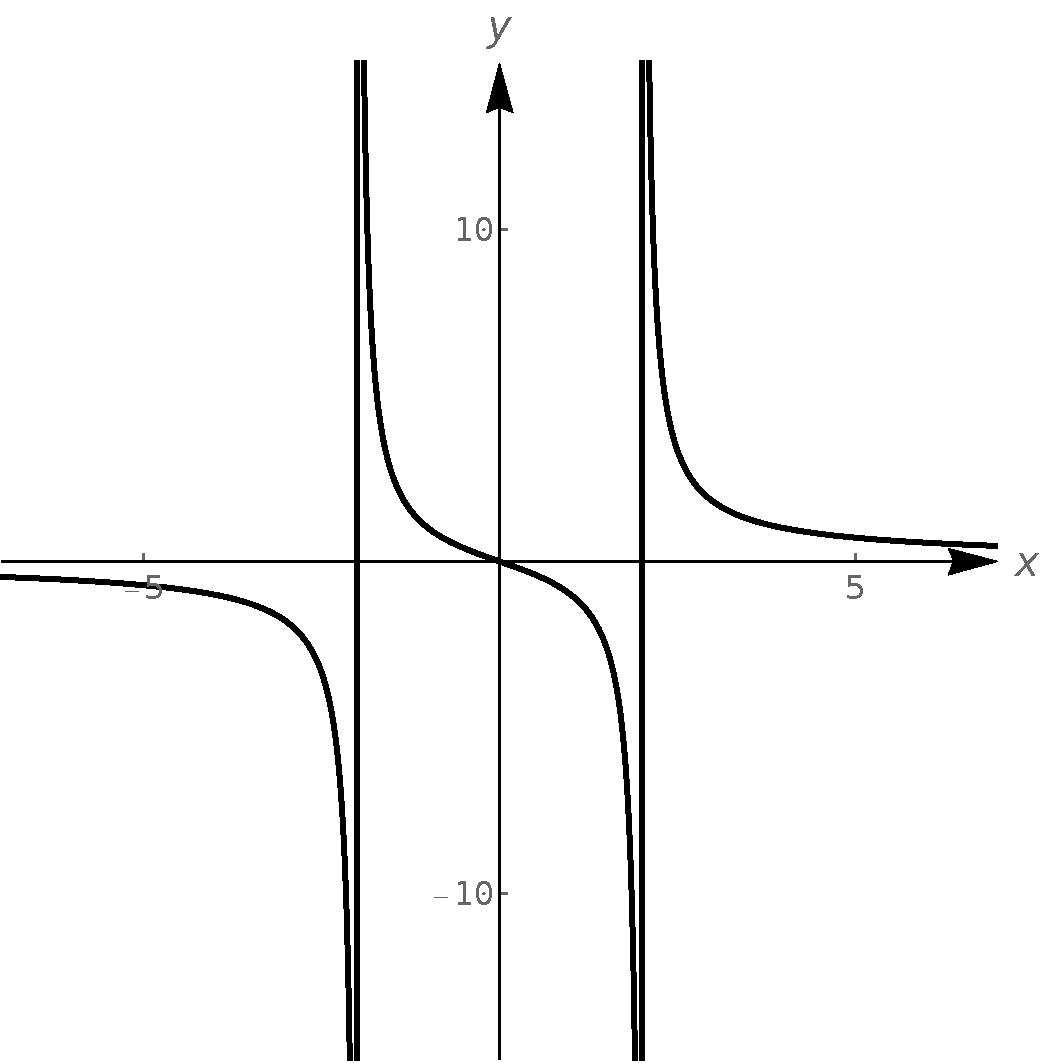
\includegraphics[width=0.4\textwidth]{fig_lim_20}
	\caption{Graphing $f(x) = \frac{3x}{x^2-4}$. }
	\label{fig_lim_20}
	\end{center}
\end{figure}


\end{example}

%When a rational function has a vertical asymptote at $x=c$, we can conclude that the denominator is 0 at $x=c$. However, just because the denominator is 0 at a certain point does not imply there is a vertical asymptote there.  For instance, the function 
%$$f(x)=\dfrac{x^2-1}{x-1}$$
% does not have a vertical asymptote at $x=1$, as shown in Figure~\ref{fig_lim_19}.  While the denominator does get small near $x=1$, the numerator gets small too, matching the denominator step for step. In fact, factoring the numerator, we get
%$$f(x)=\frac{(x-1)(x+1)}{x-1}.$$
%Cancelling the common term, we get that $f(x)=x+1$ for $x\not=1$.   So there is clearly no asymptote; rather, a hole exists in the graph at $x=1$.
%
%\begin{figure}
%	\begin{center}
%			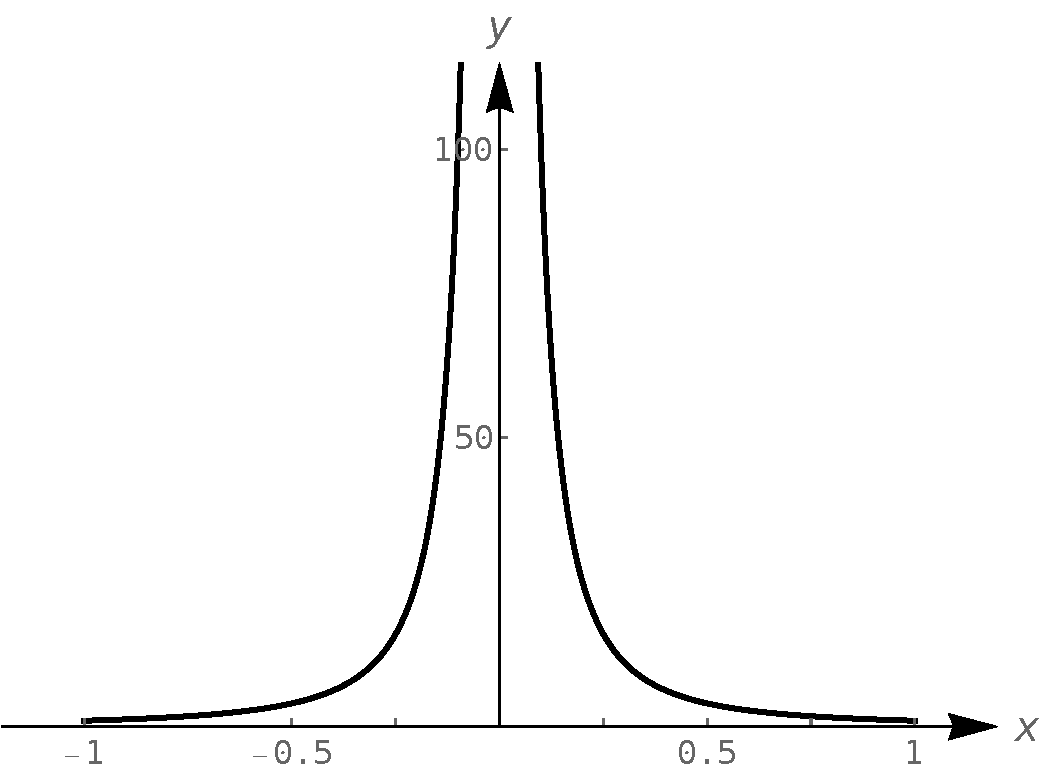
\includegraphics[width=0.4\textwidth]{fig_lim_19}
%	\caption{Graphing $f(x)=\dfrac{x^2-1}{x-1}$. }
%	\label{fig_lim_19}
%	\end{center}
%\end{figure}
%
%The above example may seem a little contrived.  Another example demonstrating this important concept is $f(x)= (\sin x)/x$. for which we found that $ \lim_{x\to0}\frac{\sin x}{x}=1$; i.e., there is no vertical asymptote. No simple algebraic cancellation makes this fact obvious though. 

If the denominator of a rational function is 0 at a certain point but the numerator is not, then there will usually be a vertical asymptote at that point.  On the other hand,  if the numerator and denominator are both zero at that point, then there may or may not be a vertical asymptote at that point.  This case where the numerator and denominator are both zero returns us to an important topic.


\ifcourse
\subsection{Indeterminate forms}
We have seen how the limits 
$$\lim_{x\rightarrow 0}\frac{\sin (x)}{x}\quad \text{and}\quad \lim_{x\to1}\frac{x^2-1}{x-1}$$ each return the indeterminate form $0/0$ when we blindly plug in $x=0$ and $x=1$, respectively. However, $0/0$ is not a valid arithmetical expression.  With a little cleverness, one can come up with $0/0$ expressions which have a limit of $\infty$, 0, or any other real number.  That is why this expression is called \textbf{indeterminate} (\textit{onbepaald}). \index[aut]{limiet ! onbepaald}\index{limit ! indeterminate}

A key concept to understand is that such limits do not really return $0/0$. Rather, keep in mind that we are taking limits. What is really happening is that the numerator is shrinking to 0 while the denominator is also shrinking to 0. The respective rates at which they do this are very important and determine the actual value of the limit.

An indeterminate form indicates that one needs to do more work in order to compute the limit. That work may be algebraic (such as factoring and cancelling) or it may require a tool such as the squeeze theorem. In Chapter~\ref{chap_diff} we will learn a technique called l'H\^opital's Rule that provides another way to handle indeterminate forms.  
 
Some other common indeterminate forms are $+\infty-\infty$, $\infty\cdot 0$, $\infty/\infty$, $0^0$, $\infty^0$ and $1^{\infty}$. Again, keep in mind that the expression $\infty-\infty$ does not really mean subtract infinity from infinity. Rather, it means one quantity is subtracted from the other, but both are growing without bound. What is the result? It is possible to get every value between $-\infty$ and $+\infty$.

\fi

\subsection{Limits at infinity and horizontal asymptotes}

In Figure~\ref{fig_lim_19} we briefly considered what happens to $f(x) = x^{-2}$ as $x$ grew very large. Graphically, it concerns the behaviour of the function to the far right of the graph. We make this notion more explicit in the following definition.


\begin{definition}[Limits at infinity and horizontal asymptotes]\label{def:limit_at_infinity}
Let $L$ be a real number.
\begin{enumerate}
\item Let $f$ be a function defined on $]a,+\infty[$ for some number $a$. The limit of $f$ at infinity is $L$, or $\ds\lim_{x\rightarrow+\infty} f(x)=L$, means for every $\varepsilon>0$ there exists $M>a$ such that if $x > M$, then $|f(x)-L|<\varepsilon$.

\item Let $f$ be a function defined on $]-\infty,b[$ for some number $b$. The limit of $f$ at negative infinity is $L$, or $\ds\lim_{x\rightarrow-\infty} f(x)=L$, means for every $\varepsilon>0$ there exists $M<b$ such that if $x < M$, then $|f(x)-L|<\varepsilon$. \\

 \item  If $\ds\lim_{x\rightarrow+\infty} f(x)=L$ or $\ds\lim_{x\rightarrow-\infty} f(x)=L$, we say the line $y=L$ is a \textbf{horizontal asymptote} (\textit{horizontale asymptoot}) of $f$.
\end{enumerate}

\index{asymptote ! horizontal}\index{horizontal asymptote}\index[aut]{ asymptoot  ! horizontale}\index[aut]{horizontale  asymptoot }
\end{definition}

Horizontal asymptotes can take on a variety of forms. Figure~\ref{fig_lim_21a} shows that $f(x) = x/(x^2+1)$ has a horizontal asymptote of $y=0$, where 0 is approached from both above and below. On the other hand, Figure \ref{fig_lim_21b} shows that $f(x) =x/\sqrt{x^2+1}$ has two horizontal asymptotes; one at $y=1$ and the other at $y=-1$. Figure \ref{fig_lim_21c} shows that $f(x) = (\sin (x))/x$ has even more interesting behaviour than at just $x=0$; as $x$ approaches $\pm\infty$, $f(x)$ approaches 0, but oscillates as it does this.\\% 

\begin{figure}
%\raisebox{0.5cm}{
\centerline{
\subfigure[\label{fig_lim_21a}]{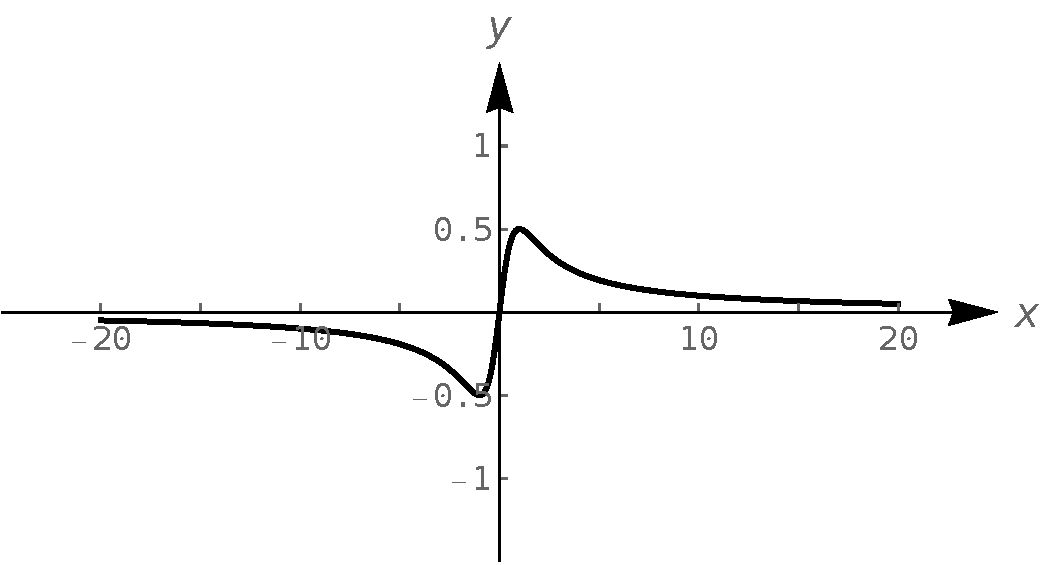
\includegraphics[width=0.3\textwidth]{fig_lim_21a}}
\qquad
\subfigure[\label{fig_lim_21b}]{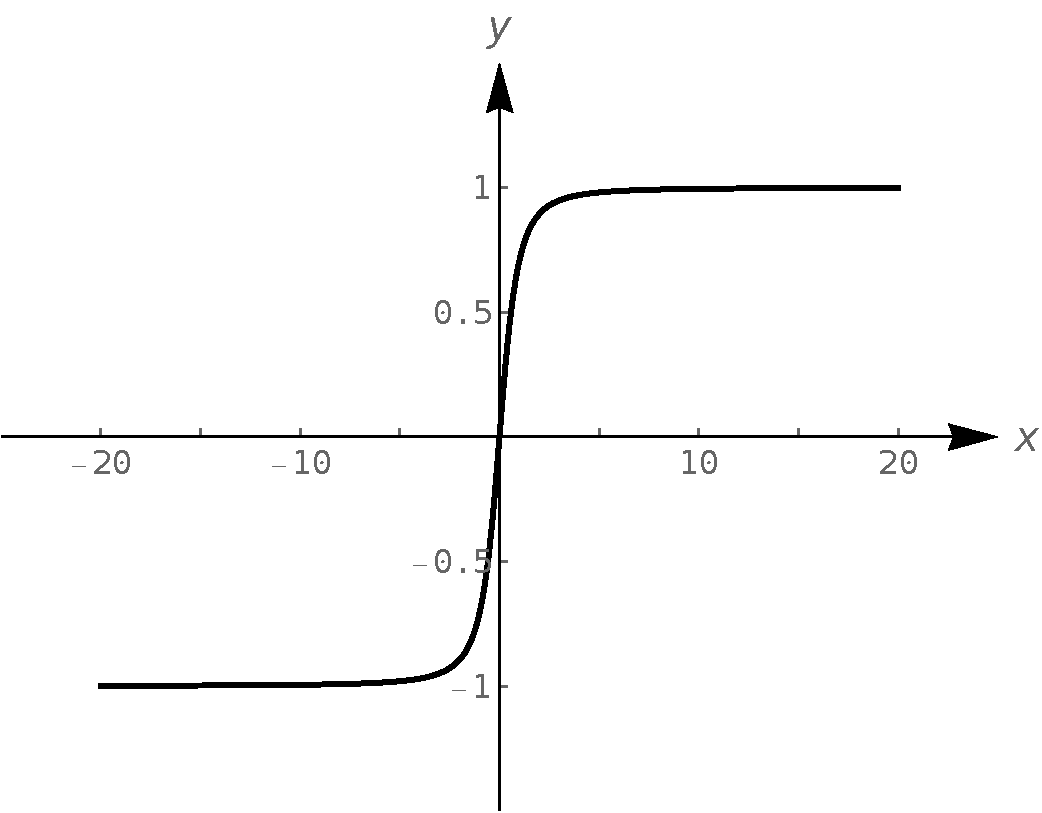
\includegraphics[width=0.3\textwidth]{fig_lim_21b} }
\qquad
\subfigure[\label{fig_lim_21c}]{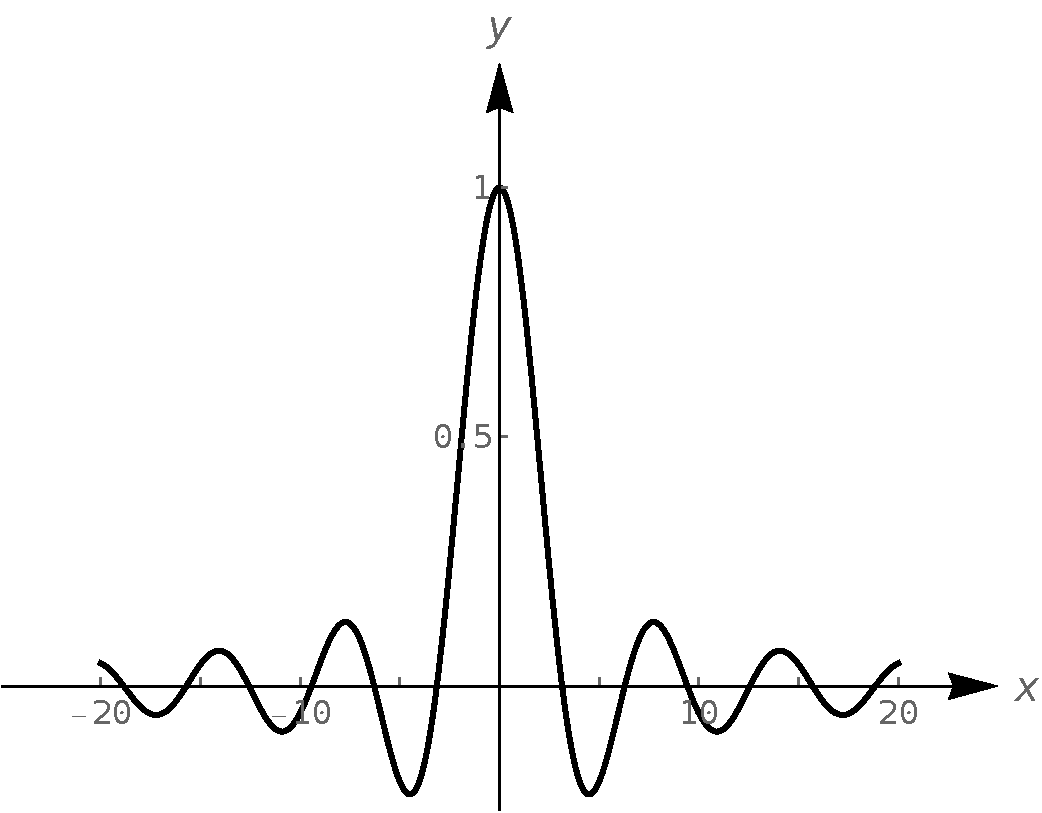
\includegraphics[width=0.3\textwidth]{fig_lim_21c} }
}
\caption{A graph of $f(x) = x/(x^2+1)$ (a), $f(x) =x/\sqrt{x^2+1}$ (b) and $f(x) = (\sin (x))/x$. }
\end{figure}


We can analytically evaluate limits at infinity for rational functions once we understand $\ds\lim_{x\rightarrow+\infty} 1/x$.  As $x$ gets larger and larger,   $1/x$ gets smaller and smaller, approaching 0.  We can, in fact, make $1/x$ as small as we want by choosing a large enough value of $x$.  Given $\varepsilon$, we can make $1/x<\varepsilon$  by choosing $x>1/\varepsilon$.  Thus we have $\ds\lim_{x\rightarrow+\infty} 1/x=0$.  It is now not much of a jump to conclude the following:
$$\lim_{x\rightarrow+\infty}\frac1{x^n}=0\quad \text{and}\quad \lim_{x\rightarrow-\infty}\frac1{x^n}=0.$$

Now suppose we need to compute the following limit:
$$\lim_{x\rightarrow+\infty}\frac{x^3+2x+1}{4x^3-2x^2+9}.$$
A good way of approaching this is to divide through the numerator and denominator by $x^3$, which is the largest power of $x$ to appear in the function.  Doing this, we get
$$
\lim_{x\rightarrow+\infty}\frac{x^3+2x+1}{4x^3-2x^2+9} = \lim_{x\rightarrow+\infty}\frac{x^3\left(1+2/x^2+1/x^3\right)}{x^3\left(4-2/x+9/x^3\right)}.
$$
Then using the rules for limits (which also hold for limits at infinity), as well as the fact about limits of $x^{-n}$, we see that the limit becomes
$$\frac{1+0+0}{4-0+0}=\frac14.$$

This procedure works for any rational function.  In fact, it gives us the following theorem.

\begin{theorem}[Limits of rational functions at infinity]\label{thm:lim_rational_fn_at_infty}
Let $f(x)$ be a rational function of the following form:
$$f(x)=\frac{a_nx^n + a_{n-1}x^{n-1}+\dots + a_1x + a_0}{b_mx^m + b_{m-1}x^{m-1} + \dots + b_1x + b_0},$$
where any of the coefficients may be 0 except for $a_n$ and $b_m$.
\begin{enumerate}
\item If $n=m$, then $\ds\lim_{x\rightarrow+\infty} f(x) = \lim_{x\rightarrow-\infty} f(x) = \frac{a_n}{b_m}$.
\item If $n<m$, then $\ds\lim_{x\rightarrow+\infty} f(x) = \lim_{x\rightarrow-\infty} f(x) = 0$.
\item If $n>m$, then $\ds\lim_{x\rightarrow+\infty} f(x)$ and $\ds\lim_{x\rightarrow-\infty} f(x)$ are both infinite.
\end{enumerate}
\end{theorem}
Intuitively, as $x$ gets very large, all the terms in the numerator are small in comparison to $a_nx^n$, and likewise all the terms in the denominator are small compared to $b_nx^m$.  If $n=m$, looking only at these two important terms, we have $(a_nx^n)/(b_nx^m)$.  This reduces to $a_n/b_m$.  If $n<m$, the function behaves like $a_n/(b_mx^{m-n})$, which tends toward 0.  If $n>m$, the function behaves like $a_nx^{n-m}/b_m$, which will tend to either $+\infty$ or $-\infty$ depending on the values of $n$, $m$, $a_n$, $b_m$ and whether you are looking for $\lim\limits_{x\rightarrow+\infty} f(x)$ or $\lim\limits_{x\rightarrow-\infty} f(x)$.

With care, we can quickly evaluate limits at infinity for a large number of functions by considering the largest powers of $x$. This is, for instance, the case for irrational functions.  As an example, consider again 
$$\ds\lim_{x\to\pm\infty}\frac{x}{\sqrt{x^2+1}},$$
graphed in Figure~\ref{fig_lim_21b}. When $x$ is very large, $x^2+1 \approx x^2$. Thus 
$$\sqrt{x^2+1}\approx \sqrt{x^2} = |x|,\quad \text{and}\quad \frac{x}{\sqrt{x^2+1}} \approx \frac{x}{|x|}.$$
 This expression is 1 when $x$ is positive and $-1$ when $x$ is negative. Hence we get asymptotes of $y=1$ and $y=-1$, respectively. In general, when evaluation limits at infinity involving irrational functions we should bear in mind that 
\[ 
\begin{array}{rcll}
\sqrt{x^2}&=&x, \quad & \forall\, x\in\mathbb{R}^+,\\  
\sqrt[3]{x^3}&=&x, \quad& \forall \, x\in\mathbb{R},\\
\sqrt{x^2}&=&-x, \quad & \forall\, x\in\mathbb{R}^-,\\
\sqrt[3]{(-x)^3}&=&-x, \quad& \forall \, x\in\mathbb{R}.
\end{array}
\] 

\begin{example}\label{ex_hzasy3}
Evaluate each of the following limits.

\begin{multicols}{2}
\begin{enumerate}
\item		$\displaystyle\lim_{x\rightarrow-\infty}\frac{x^2+2x-1}{x^3+1}$
\item		$\displaystyle\lim_{x\rightarrow+\infty}\frac{x^2-1}{3-x}$
\item $\ds\lim_{x\rightarrow -\infty}\dfrac{\sqrt{x^2+5}+7x}{2x-3}$
\item $\ds\lim_{x\rightarrow -\infty}\left( \sqrt{x^2+8x}+x\right)$
\ifcourse \ifanalysis \item $\ds\lim_{x\rightarrow +\infty}\left( \cosh(x)-\sinh(x)\right)$\fi \fi
\end{enumerate}
\end{multicols}

\xhrulefill{gray}{2.5pt}Solution \xhrulefill{gray}{2.5pt}

	\begin{enumerate}
	\item		The highest power of $x$ is in the denominator.  Therefore, the limit is 0.	
	\item		We see that
	\begin{eqnarray*}
	\displaystyle\lim_{x\rightarrow+\infty}\frac{x^2-1}{3-x}&=&\displaystyle\lim_{x\rightarrow+\infty}\frac{x^2\left(1-1/x^2\right)}{x\left(3/x-1\right)}\\
	&=&\displaystyle\lim_{x\rightarrow+\infty}\frac{x\left(1-1/x^2\right)}{3/x-1}=-\infty\,.\\
	\end{eqnarray*}
	\item We first should realize that the highest power of $x$ in both the numerator and denominator is the same.  Hence, we proceed as follows:
	
	\begin{eqnarray*}
	\ds\lim_{x\rightarrow -\infty}\dfrac{\sqrt{x^2+5}+7x}{2x-3}&=&
	\ds\lim_{x\rightarrow -\infty}\dfrac{  |x| \sqrt{1+\dfrac{5}{x^2}}+7x }{x\left(2-\dfrac{3}{x}\right)}\\
&=&\ds\lim_{x\rightarrow -\infty}\dfrac{  x \; \left(- \sqrt{1+\dfrac{5}{x^2}}+7\right) }{x\left(2-\dfrac{3}{x}\right)}\\
&=&\dfrac{-1+7}{2}=3.
\end{eqnarray*}

\item At first sight, we would say that this limit leads to the indeterminate form $\infty-\infty$, but this can be overcome by multiplying both numerator and denominator by the conjugate expression. 
\begin{eqnarray*}
\ds\lim_{x\rightarrow -\infty}\left( \sqrt{x^2+8x}+x\right) & =& \ds\lim_{x\rightarrow -\infty} \dfrac{x^2+8x-x^2}{\sqrt{x^2+8x}-x} \\
&=& \ds\lim_{x\rightarrow -\infty} \dfrac{8x}{-x\left(\sqrt{1+\dfrac{8}{x}}+1\right)} = \dfrac{8}{-2} = -4
\end{eqnarray*}
\ifcourse
\ifanalysis \item At first sight, this limit returns the indeterminate form $\infty-\infty$, but we can try to work around it by multiplying the nominator and denominator with the conjugate binomial \\ $\cosh(x)+\sinh(x)$. This leads to 
\begin{eqnarray}
\ds\lim_{x\rightarrow +\infty}\left( \cosh(x)-\sinh(x)\right)&=&\ds\lim_{x\rightarrow +\infty}\dfrac{ \cosh^2(x)-\sinh^2(x)}{\cosh(x)+\sinh(x)}\\
&=&\ds\lim_{x\rightarrow +\infty}\dfrac{1}{\cosh(x)+\sinh(x)}\\
&=&0\,.
\end{eqnarray}

 \fi
 \fi
\end{enumerate}

\ifmathematica
\ifcourse
In Mathematica, these limits are again computed as any other limit. To specify that the limit is at (minus) infinity, we simply write \lstinline{(-)Infinity}. For example, 
$$\displaystyle\lim_{x\rightarrow-\infty}\frac{x^2+2x-1}{x^3+1},$$
is computed as follows.
\begin{mdframed}[default,backgroundcolor=gray!40,roundcorner=8pt]
\begin{mmaCell}[morefunctionlocal={x},moredefined={Direction}]{Input}
  Limit[(x^2 + 2 x - 1) (x^3 + 1), x -> -Infinity]
\end{mmaCell}

\begin{mmaCell}{Output}
  \(0\)
\end{mmaCell}
\end{mdframed}
\fi
\fi

\ifpython
\ifcourse
In Python, these limits are again computed as any other limit. To specify that the limit is at (minus) infinity, we simply write \lstinline{(-)Infinity}. For example, 
$$\displaystyle\lim_{x\rightarrow-\infty}\frac{x^2+2x-1}{x^3+1},$$
is computed as follows.
\begin{pyin}
from sympy import limit, symbols, oo
x = symbols('x')
limit((x**2 + 2*x - 1)/(x**3 + 1), x, -oo)
\end{pyin}
\begin{pyout}
0
\end{pyout}
\fi
\fi
\end{example}

For the sake of comprehensiveness, we list below the steps that should be taken when evaluating the limit $\dlim_{x\to \pm \infty} f(x)$:

\begin{enumerate}
\item Compute $f(\pm \infty)$.  
\item You arrive at one of the following cases:
\begin{itemize}
\item $f(\pm \infty) = \pm \infty$: the function values approaches $\infty$ as $x\to \pm \infty$
\item $ f(\pm \infty) = b \in\mathbb{R}$: $y=b$ is a horizontal asymptote of the function $f$.  
\item  $f(\pm \infty) = \left(\frac{\infty}{\infty}\right)$: factor out the highest-degree term in both the nominator and denominator, then simplify and return to Step 1. 
\item $f(\pm \infty) = (\infty - \infty)$: multiply with the conjugate binomial, then factor out the highest-degree term and return to Step 1.
\end{itemize}
\end{enumerate}



\ifcourse
\subsection{Slant asymptotes}
In addition to vertical and horizontal asymptotes, we can also define \textbf{slant or oblique asymptotes} (\textit{schuine asymptoot}). These are diagonal lines such that the difference between the curve and the line approaches 0 as $x$ tends to $+\infty$ or $-\infty$. 
\index{asymptote ! slant}\index{slant asymptote}\index{asymptote ! oblique}\index{oblique asymptote}\index[aut]{ asymptoot  ! schuine}\index[aut]{schuine  asymptoot }

\begin{definition}[Slant asymptotes]\label{def:slant}
The line $y=ax+b$ is a \textbf{slant asymptote} for the function $f$ if and only if
 $$\ds\lim_{x\rightarrow+\infty} \left[f(x)-\left(ax+b\right)\right]=0,$$ 
or/and
$$\ds\lim_{x\rightarrow-\infty} \left[f(x)-\left(ax+b\right)\right]=0\,.$$

\index{asymptote ! horizontal}\index{horizontal asymptote}\index[aut]{ asymptoot  ! horizontale}\index[aut]{horizontale  asymptoot }
\end{definition}
From this definition, it follows that 
\[ \ds\lim_{x\rightarrow\pm\infty}\left[ \dfrac{f(x)}{x} -\left( a+\dfrac{b}{x}\right)\right]=0, \]
so
\[ a=\ds\lim_{x\rightarrow\pm\infty}\dfrac{f(x)}{x} \qquad \text{ and } \qquad b=\ds\lim_{x\rightarrow\pm\infty}(f(x)-ax) \, . \]


\begin{example}
Determine the asymptotes, if any, of the following functions.
\begin{multicols}{2}
\begin{enumerate}
\item $f(x)=\dfrac{x^3+2}{x^2-9}$
\item $f(x)=\sqrt{x^2-4x+3}$
\end{enumerate}
\end{multicols}

\xhrulefill{gray}{2.5pt}Solution \xhrulefill{gray}{2.5pt}

\begin{enumerate}
\item 
\begin{enumerate}
\item Vertical asymptotes\\

Since $f(x)$ tends to infinity as $x$ approaches 3 or $-3$, the vertical asymptotes are $x=-3$ and $x=3$. More precisely, we find that 
\[
\begin{array}{ll}
\ds\lim_{x\underset{<}{\rightarrow}-3} f(x) = - \infty  &\quad \quad \quad \ds\lim_{x\underset{<}{\rightarrow}3} f(x) = - \infty \\
\ds\lim_{x\underset{>}{\rightarrow}-3} f(x) = + \infty  &\quad \quad  \quad \ds\lim_{x\underset{>}{\rightarrow}3} f(x) = + \infty
\end{array}
\]
This allows us to conclude that $f(x)$ tends towards $-\infty$ as $x$ is approaching $-3$ from the left, whereas $f(x)$ tends towards $\infty$ when approaching $-3$ from the right, and likewise for what concerns the vertical asymptote at $x=3$. 
\item Horizontal asymptotes\\

There are none because
\[ \ds\lim_{x \rightarrow \pm \infty} \dfrac{x^3+2}{x^2-9} = \pm \infty. \]

\item Slant asymptotes\\

We verify that 
\[a = \ds\lim_{x \rightarrow \pm \infty} \dfrac{f(x)}{x} = \ds\lim_{x \rightarrow \pm \infty} \dfrac{x^3+2}{x^3-9x} = 1, \]
\[b = \ds\lim_{x \rightarrow \pm \infty} \left(f(x) - ax \right) = \ds\lim_{x \rightarrow \pm \infty} \left( \dfrac{x^3+2}{x^2-9} - x  \right) = \ds\lim_{x \rightarrow \pm \infty} \left( \dfrac{2+9x}{x^2-9}\right) = 0.  \]

Consequently, the function has slant asymptote $y=x$ for $x \rightarrow \pm \infty$. The position of this asymptote with respect to the graph of the function $f$ can be found be determining the sign of 
\[
g(x) = f(x) - (ax+b)  = \dfrac{x^3+2}{x^2-9} - x =  \dfrac{9x+2}{x^2-9} .
\]


The sign diagram of the function $g$ is:
\[
\begin{array}{c||ccccccc}
			x &  & -3& & -\frac{2}{9}& & 3 &   \\
			\hline
			g(x) & - & | & + & 0 & - & | & + 
			\end{array}
\]

Consequently, we may conclude that the graph of $f$ lies above the slant asymptote for $x \rightarrow +\infty$ because then $g(x) > 0$, whereas the graph of $f$ lies below the slant asymptote for $x \rightarrow -\infty$ because then $g(x) < 0$. This is confirmed by the graph of the function $f$ shown in Figure~\ref{fig_lim_22a}.
\end{enumerate}
\item $f(x)=\sqrt{x^2-4x+3}$
\begin{enumerate}
\item Vertical asymptotes\\

The function $f(x)$ only tends to infinity if $x$ does so, so there are no vertical asymptotes. 
\item Horizontal asymptotes\\

There are none because
\[ \ds\lim_{x \rightarrow \pm \infty} \sqrt{x^2-4x+3} = +\infty. \]

\item Slant asymptotes\\

We verify that
\begin{itemize}
\item $x\rightarrow +\infty$
\[a\; =\; \ds\lim_{x \rightarrow + \infty} \dfrac{f(x)}{x}\; =\; \ds\lim_{x \rightarrow + \infty} \dfrac{\sqrt{x^2-4x+3}}{x}\; =\; 1, \]
\begin{eqnarray*}
b & = & \ds\lim_{x \rightarrow + \infty} \left(f(x) - ax \right)\; =\; \ds\lim_{x \rightarrow + \infty} \left( \sqrt{x^2-4x+3} - x  \right)\\
& = & \ds\lim_{x \rightarrow + \infty} \left( \dfrac{-4x+3}{\sqrt{x^2-4x+3} + x}\right)\; =\; -2.
\end{eqnarray*}

\item $x\rightarrow -\infty$
\[a\; =\; \ds\lim_{x \rightarrow - \infty} \dfrac{f(x)}{x}\; =\; \ds\lim_{x \rightarrow - \infty} \dfrac{\sqrt{x^2-4x+3}}{x}\; =\; -1, \]
\begin{eqnarray*}
b & = & \ds\lim_{x \rightarrow - \infty} \left(f(x) - ax \right)\; =\; \ds\lim_{x \rightarrow - \infty} \left( \sqrt{x^2-4x+3} + x  \right)\\
& = & \ds\lim_{x \rightarrow - \infty} \left( \dfrac{-4x+3}{\sqrt{x^2-4x+3} - x}\right)\; =\; 2.
\end{eqnarray*}
\end{itemize}

Hence,  $y=x-2$ is a slant asymptote of $f$ for $x \rightarrow + \infty$, while $y=-x+2$ is a slant asymptote of $f$  for $x \rightarrow -\infty$. Again, the position of the slant asymptote with respect to the graph of $f$ can be determined by verifying the sign of 
\[
g(x) = \sqrt{x^2-4x+3}  - (x-2) %=  \dfrac{-1}{\sqrt{x^2-4x+3} + (x-2)} 
%\]
\qquad\mbox{and}\qquad% van
%\[
h(x) = \sqrt{x^2-4x+3} - (-x+2) %=  \dfrac{-1}{\sqrt{x^2-4x+3} + (-x+2)} 
.\]
It follows that as $x \rightarrow +\infty$, then we have that  $g(x) < 0$, so the graph of $f$ lies below the slant asymptote $y=x-2$. Similarly, as  $x \rightarrow -\infty$, then we have that $h(x) < 0$, so the graph of $f$ lies below the slant asymptote $y=-x+2$. This is confirmed by the graph of the function $f$ shown in Figure~\ref{fig_lim_22b}.

\end{enumerate}

\end{enumerate}

\begin{figure}[H]
%\raisebox{0.5cm}{
\centerline{
\subfigure[\label{fig_lim_22a}]{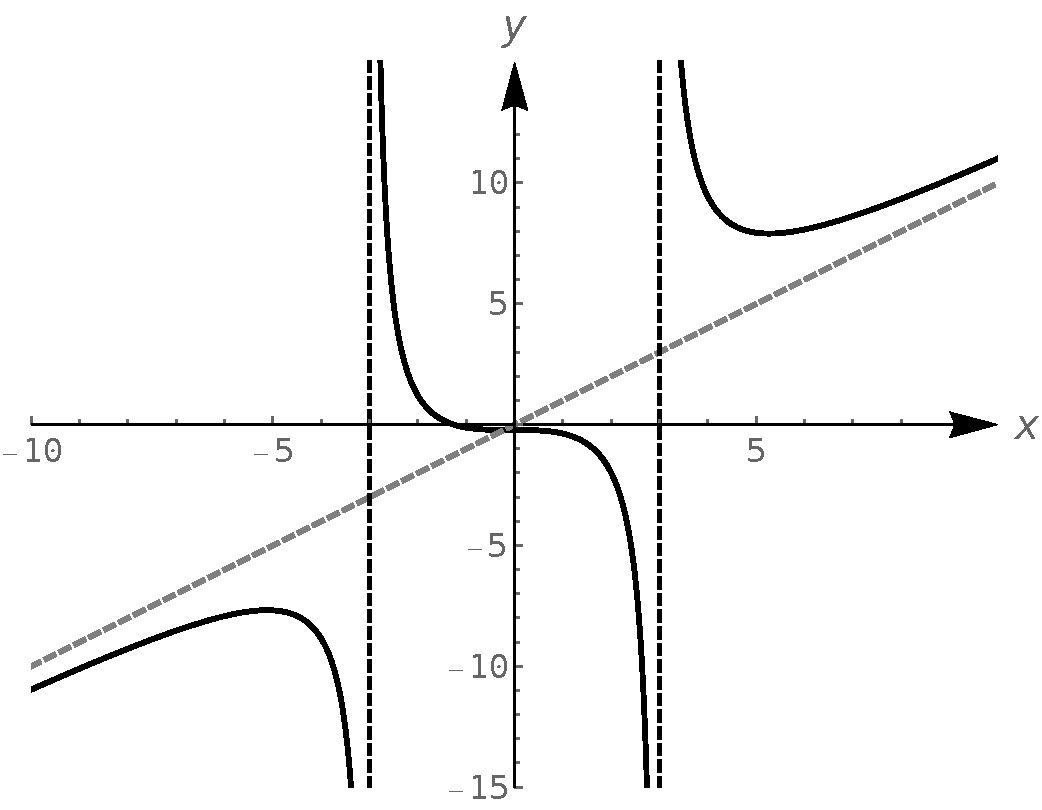
\includegraphics[width=0.4\textwidth]{fig_lim_22a}}
\qquad
\subfigure[\label{fig_lim_22b}]{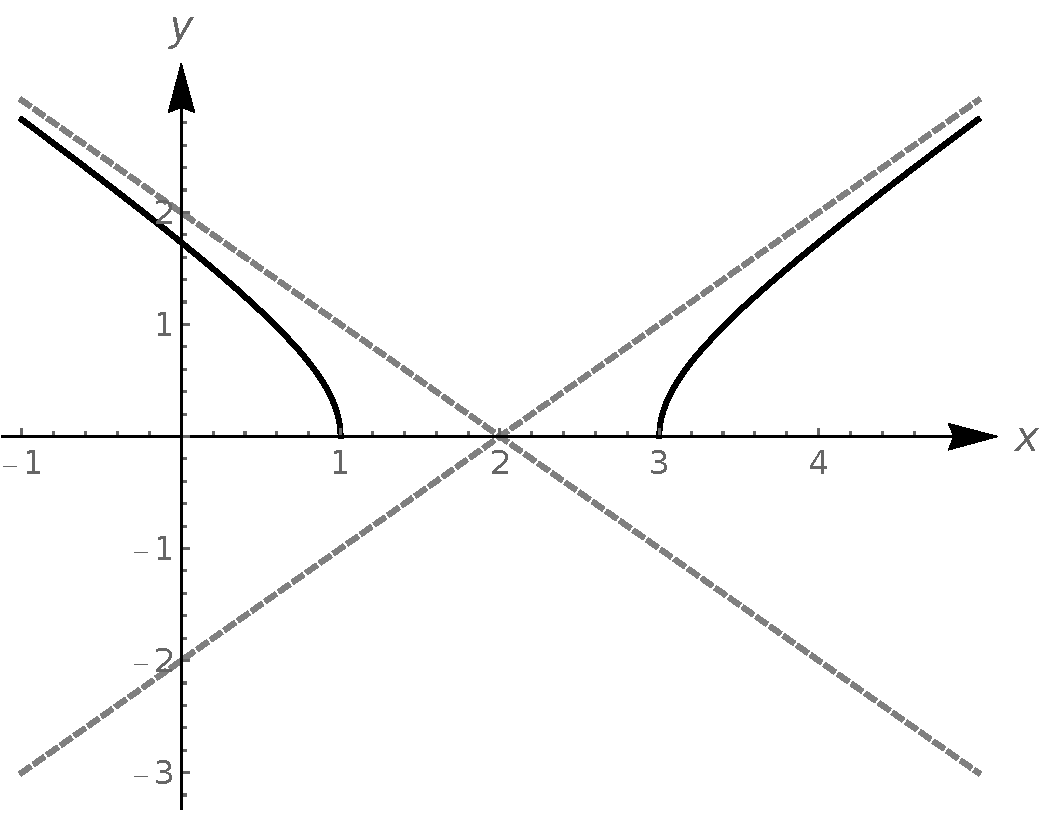
\includegraphics[width=0.4\textwidth]{fig_lim_22b} }
}
\caption{A graph of $f(x)=\frac{x^3+2}{x^2-9}$ (a) and $f(x)=\sqrt{x^2-4x+3}$ (b). }
\end{figure}
\end{example}

\fi


%%%%%%%%%%%%%%%%%%%%%
% Oefeningen cursus
%%%%%%%%%%%%%%%%%%%%%

\ifcourse
\newpage
\section{Exercises}

\renewcommand{\ExerciseListName}{Assignement}


\ifanalysis

\subsection*{\nameref{sec:limit_def}}
%%%%%%%%%%%%%%%%%%%%
%Oefening 1 Bio-irs
%%%%%%%%%%%%%%%%%%%
\begin{Exercise}[difficulty = 2] Consider
    \[ f(x)=\sqrt{2x+3}, \quad c=3, \quad L=3, \quad \varepsilon=0,01. \]
   Find a $\delta > 0$ such that $|x-c| < \delta $, $|f(x) - L|$ is smaller than the given $\varepsilon$.  

\end{Exercise}

\setboolean{firstanswerofthechapter}{true}
\begin{Answer}\phantom{}
    Prove with the $(\varepsilon,\,\delta)$-definition.
\end{Answer}
\setboolean{firstanswerofthechapter}{false}
    
%%%%%%%%%%%%%%%%%%%%
%Oefening 2 Bio-irs
%%%%%%%%%%%%%%%%%%%
\begin{Exercise} Prove the given limit by using the $(\varepsilon,\,\delta)$-definition (Definition~\ref{def:limit}).
    \begin{multicols}{3}
        \Question[difficulty = 1] $\dlim_{x\rightarrow 5} (3-x) = -2 $
        \Question[difficulty = 2] $\dlim_{x\rightarrow 4} \left(x^2+x-5\right) = 15 $
        \Question[difficulty = 1] $\dlim_{x\rightarrow 0} \sin (x) = 0 $
        \EndCurrentQuestion
    \end{multicols}

\end{Exercise}

\begin{Answer}\phantom{}
    \begin{multicols}{3}
    
        \Question Choose $\delta = \varepsilon$.
        \Question Choose $\delta = \dfrac{\varepsilon}{10}$.
        \Question Choose $\delta = \varepsilon$.
    \EndCurrentQuestion
    \end{multicols}
\end{Answer}
    
\subsection*{\nameref{sec:berekenen_lim}}

%%%%%%%%%%%%%%%%%%%%
%Oefening 3 Bio-irs
%%%%%%%%%%%%%%%%%%%
\begin{Exercise}[difficulty = 2] Prove the product rule for limits. If
    \[\dlim_{x\rightarrow c} f(x) = L _1 \quad  \text{ and } \quad  \dlim_{x\rightarrow c} g(x) = L_2, \]
    than
    \[\dlim_{x\rightarrow c} f(x)g(x) = L_1L_2 \] or:
    \[\dlim_{x\rightarrow c} f(x)g(x) = \dlim_{x\rightarrow c} f(x) \dlim_{x\rightarrow c} g(x). \]

\end{Exercise}

\begin{Answer}\phantom{}
    Prove similar to sum. \\
    Hint: 
    \begin{eqnarray*}
    |f(x)g(x) - L_1 L_2| &=& |f(x)g(x) - L_1 g(x) + L_1 g(x) - L_1 L_2| \\
    &=& |(f(x) - L_1)g(x) + L_1(g(x) - L_2)| \\
    &\leq& |(f(x) - L_1)g(x)| + |L_1(g(x) - L_2)| \\
    &=& |g(x)||f(x) - L_1| + |L_1||g(x) - L_2|
    \end{eqnarray*}
    Make each term in the last line smaller than $\varepsilon/2$ by choosing $x$ close enough to $c$. 
    %Gebruik hierbij het resultaat uit oefening 32, namelijk %\[ 0<|x-a|<\delta \quad\Rightarrow\quad |g(x)|<1+|M|. \]
\end{Answer}
    
\fi


%%%%%%%%%%%%%%%%%%%%
%Oefening 4 Bio-irs
%Oefening 1 Ings
%%%%%%%%%%%%%%%%%%%
\begin{Exercise} Calculate the following limits. 
 \begin{multicols}{2} 
        \ifcalculus
        \Question[difficulty = 1] $\dlim_{x\rightarrow -1} \left(4x^2-5x+3\right)$
        \Question[difficulty = 1] $\dlim_{x\underset{>}{\rightarrow}0} x^2\ln(x)$
        \Question[difficulty = 1] $\dlim_{x\rightarrow 1} \dfrac{x^2-1}{x^3-1} $
        \Question[difficulty = 1] $\dlim_{x\rightarrow 2} \dfrac{\sqrt{x+2}-2}{x-2}$
        \fi
		\Question[difficulty = 1] $\dlim_{x\underset{>}{\rightarrow}1} \dfrac{\sqrt{(x-1)^2}}{x-1}$
		\Question[difficulty = 1] $\dlim_{x\underset{>}{\rightarrow}-4}\dfrac{2x+8}{|x+4|}$
		\Question[difficulty = 1] $\dlim_{x\rightarrow 1}\dfrac{(x-1)^3}{x^2-4x+3}$
		\Question[difficulty = 1] $\dlim_{x\rightarrow -1}\dfrac{x^3+2x^2+x}{x^8-2x^4+1}$
		\ifanalysis\Question[difficulty = 1]\fi\ifcalculus\Question[difficulty = 2]\fi $\dlim_{x\rightarrow 1}\dfrac{x-\sqrt{x}}{2-\sqrt{x+3}}$
		\ifanalysis\Question[difficulty = 1]\fi\ifcalculus\Question[difficulty = 2]\fi $\dlim_{x\rightarrow 5}\dfrac{\sqrt{x+4}+x-8}{x^2-8x+15}$
		\Question[difficulty = 3] $\dlim_{x\rightarrow 1}\dfrac{\sqrt{8x+1}+\sqrt{2x-1}-4}{x-1}$
		\Question[difficulty = 1] $\dlim_{x\rightarrow 0} \dfrac{|3x-1| - |3x+1|}{x}$
		\Question[difficulty = 1] $\dlim_{x\rightarrow 3} \dfrac{x^2-6x+9}{x^2-9}$
		\Question[difficulty = 1] $\dlim_{h\rightarrow 0} \dfrac{\sqrt{4+h}-2}{h}$ 
    	\Question[difficulty = 1] $\dlim_{x\rightarrow 1} \dfrac{x^2-1}{\sqrt{x+3}-2}$
        \Question[difficulty = 1] $\dlim_{x\rightarrow 2} \dfrac{x^4-16}{x^3-8}$
        \ifanalysis
        	\Question[difficulty = 1] $\dlim_{x\rightarrow 8} \dfrac{x^{2/3}-4}{x^{1/3}-2}$ 
        	\Question[difficulty = 1] $\dlim_{x\rightarrow 2} \left(\dfrac{1}{x-2} - \dfrac{1}{x^2-4} \right)$
            \Question[difficulty = 2] $\dlim_{x\rightarrow 64} \dfrac{x^{1/3}-4}{x^{1/2}-8}$
            \Question[difficulty = 2] $\dlim_{x\rightarrow 1} \dfrac{\sqrt{3+x} - 2}{\sqrt[3]{7+x} - 2}$
        \fi
        \EndCurrentQuestion
\end{multicols}

\end{Exercise}

\begin{Answer}\phantom{}
    \begin{multicols}{3} 
		
		    \ifcalculus
		    \Question $12$
		    \Question $0$
		    \Question $\dfrac{2}{3}$
		    \Question $\dfrac{1}{4}$
		    \fi
			\Question $1$
			\Question $2$
			\Question $0$
			\Question $-\dfrac{1}{16}$
			\Question $-2$ 
			\Question $\dfrac{7}{12}$
			\Question $\dfrac{7}{3}$
			\Question $-6$ 
		    \Question $0$ 
            \Question $\dfrac{1}{4}$ 
            \Question $8$ 
    	   	\Question $\dfrac{8}{3}$ 
         \ifanalysis
            \Question $4$ 
            \Question $x\underset{>}{\rightarrow}2: +\infty \; \wedge\; x\underset{<}{\rightarrow}2: - \infty$ 
            \Question $\dfrac{1}{3}$ 
            \Question $3$
         \fi
		\EndCurrentQuestion	
	\end{multicols}
\end{Answer}


%%%%%%%%%%%%%%%%%%%%
%Oefening 5 Bio-irs
%Oefening 2 Ings
%%%%%%%%%%%%%%%%%%%
\begin{Exercise}[difficulty = 1] Determine $\dlim_{x\rightarrow 0} \left( x^2 \sin \left( \dfrac{1}{x} \right) \right) $ by using the squeeze theorem.

\end{Exercise}

\begin{Answer}\phantom{}
    $\dlim_{x\rightarrow 0} \left( x^2 \sin \left( \dfrac{1}{x} \right) \right) = 0$ \\[0.2cm]
Use the fact that $-1 \leq \sin \left( \dfrac{1}{x} \right) \leq 1$, multiply both parts with $x^2$ and take the limit for $x \rightarrow 0$.
\end{Answer}

%%%%%%%%%%%%%%%%%%%%
%Oefening 6 Bio-irs
%%%%%%%%%%%%%%%%%%%
\ifanalysis
\begin{Exercise}[difficulty = 1] Assume $|f(x)| \leq g(x)$ for all $x$. What can be concluded for $\dlim_{x\rightarrow c} f(x)$ if (a) $\dlim_{x\rightarrow c} g(x)=0$ and (b) $\dlim_{x\rightarrow c} g(x)=3$?  

\end{Exercise}

\begin{Answer}\phantom{}
    \begin{multicols}{2}
    
    \Question  $\dlim_{x\rightarrow a} f(x) = 0$
    \Question  $-3 \leq \dlim_{x\rightarrow a} f(x) \leq 3$
    \EndCurrentQuestion
    \end{multicols}
\end{Answer}
\fi

\subsection*{\nameref{sec:limit_continuity}}



%%%%%%%%%%%%%%%%%%%%
%Oefening 7 Bio-irs
%Oefening 3 Ings
%%%%%%%%%%%%%%%%%%%
\begin{Exercise}[difficulty = 1, label = oef_grafiek_lim] Consider the function $y=f(x)$ as given in Figure \ref{fig_lim_23} and calculate the limits.

\begin{multicols}{3}
\Question $\dlim_{x\underset{>}{\rightarrow}  0} f(x)$ 
\Question $\dlim_{x\rightarrow 1} f(x)$
\Question $ \dlim_{x\underset{>}{\rightarrow}  2} f(x) $
\Question $ \dlim_{x\underset{<}{\rightarrow} 2} f(x)$
\Question $\dlim_{x\underset{<}{\rightarrow} 3} f(x)$
\Question $\dlim_{x\underset{>}{\rightarrow} 3} f(x) $
\Question $ \dlim_{x\underset{>}{\rightarrow} 4} f(x)$ 
\Question $\dlim_{x\underset{<}{\rightarrow}4} f(x) $
\Question $ \dlim_{x\underset{<}{\rightarrow} 5} f(x) $
\Question $ \dlim_{x\underset{>}{\rightarrow} 5} f(x)$ 
\Question $\dlim_{x\rightarrow +\infty} f(x) $
\EndCurrentQuestion 
\end{multicols}

\begin{figure}[H]
	\begin{center}
		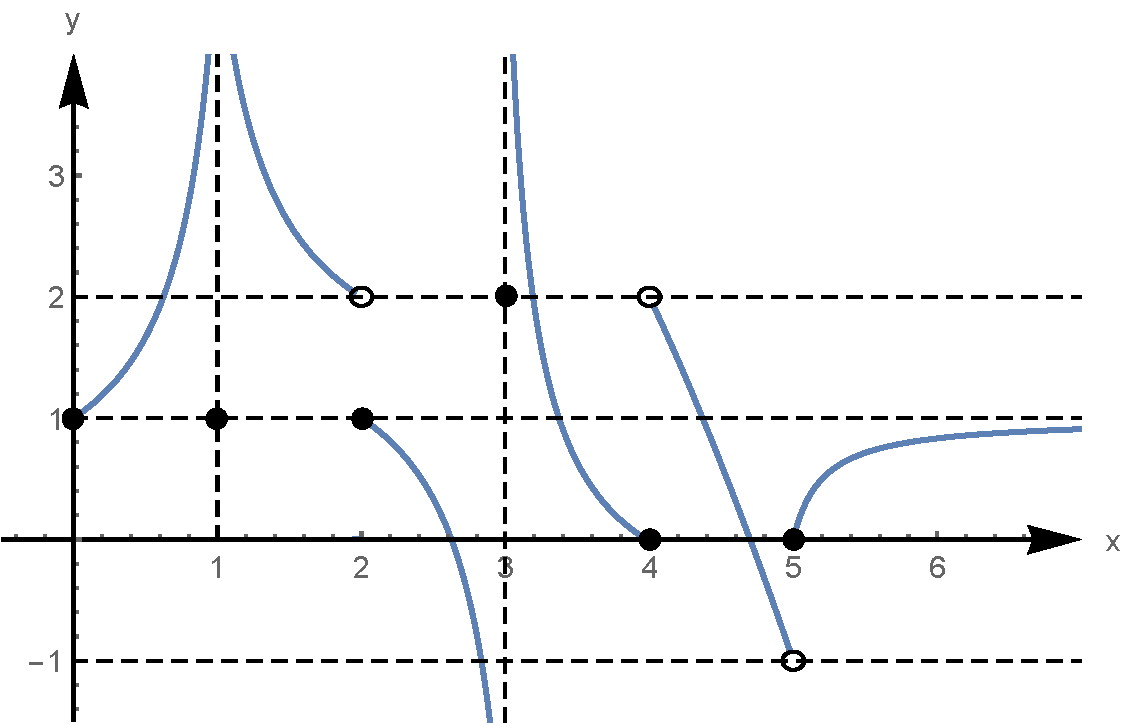
\includegraphics[scale=0.6]{fig_lim_23}
	\end{center}
	\caption{The function $y=f(x)$ from Exercise \ref{oef_grafiek_lim} \ifanalysis and \ref{oef_grafiek_cont}\fi.}
	\label{fig_lim_23}
\end{figure}

\end{Exercise}

\begin{Answer}\phantom{}
    
	\begin{multicols}{3}
		\Question $1$ 
		\Question $+ \infty$
		\Question $ 1$
		\Question $ 2$
		\Question $- \infty$
		\Question $+ \infty$
		\Question $ 2$ 
		\Question $0 $
		\Question $-1 $
		\Question $ 0$ 
		\Question $1 $
	\EndCurrentQuestion
	\end{multicols}
\end{Answer}



%%%%%%%%%%%%%%%%%%%%
%Oefening 8 Bio-irs
%Oefening 4 Ings
%%%%%%%%%%%%%%%%%%%
\begin{Exercise}[difficulty = 1] Consider the function
\[
f(x)=\left\{\begin{array}{lcl}
x-1,  & \mbox{if} & x \leq -1, \\[0.1cm]
x^2+1,  & \mbox{if} & -1 < x \leq 0, \\[0.1cm]
(x + \pi)^2,  & \mbox{if} &  x > 0 .
\end{array}\right.
\]

Compute the following limits
\begin{multicols}{2}
	\Question  $\dlim_{x\underset{<}{\rightarrow}-1} f(x)$ 
	\Question  $\dlim_{x\underset{>}{\rightarrow}-1} f(x)$ 
	\Question  $\dlim_{x\underset{>}{\rightarrow} 0} f(x)$ 
	\Question  $\dlim_{x\underset{<}{\rightarrow} 0} f(x)$ 
\EndCurrentQuestion 
\end{multicols}

\end{Exercise}

\begin{Answer}\phantom{}
    \begin{multicols}{2}
		
		\Question  $-2$ 
		\Question  $2$ 
		\Question  $\pi^2$ 
		\Question  $1$ 
		\EndCurrentQuestion
	\end{multicols}
\end{Answer}



%%%%%%%%%%%%%%%%%%%%
%Oefening 9 Bio-irs
%%%%%%%%%%%%%%%%%%%
\ifanalysis
\begin{Exercise}[difficulty = 2] If $\dlim_{x\underset{>}{\rightarrow}0} f(x) = A$ and $\dlim_{x\underset{<}{\rightarrow}0} f(x)=B$, determine
\begin{multicols}{2}
    \Question $\dlim_{x\underset{<}{\rightarrow}0} f\left(x^2-x^4\right)$,
    \Question $\dlim_{x\underset{>}{\rightarrow}0} f\left(x^2-x^4\right)$.
    \EndCurrentQuestion
\end{multicols}

\end{Exercise}

\begin{Answer}\phantom{}
    \begin{multicols}{2}
    
        \Question $\dlim_{x\underset{<}{\rightarrow}0} f(x^2-x^4)= A$  
        \Question $\dlim_{x\underset{>}{\rightarrow}0} f(x^2-x^4)= A$
    \EndCurrentQuestion
    \end{multicols}
\end{Answer}
\fi

\subsection*{\nameref{sec:continuity}}


\ifanalysis
%%%%%%%%%%%%%%%%%%%%
%Oefening 10 Bio-irs
%%%%%%%%%%%%%%%%%%%
\begin{Exercise}[difficulty = 1, label = oef_grafiek_cont] Consider Figure \ref{fig_lim_23} once more. In which points is $f(x)$ discontinuous? In which points is $f(x)$ left or right continuous? Can the function $f(x)$ be defined in $x=1$ such that $f(x)$ becomes continuous in this point? 

\end{Exercise}

\begin{Answer}\phantom{}
    $f(x)$ is discontinuous in $x=1, x=2, x=3, x=4$ and $x=5$. $f$ is left continuous in $x=4$ and right continuous in $x=2$ and $x=5$.
    $f(x)$ can not be redefined in $x=1$ such that the function becomes continuous because $\dlim_{x \rightarrow 1} f(x) = + \infty$ does not exist ($+\infty \notin \mathbb{R})$.
\end{Answer}
\fi


\ifanalysis
%%%%%%%%%%%%%%%%%%%%
%Oefening 11 Bio-irs
%%%%%%%%%%%%%%%%%%%
\pagebreak
\begin{Exercise} Determine the value of $a$ and/or $b$ such that the functions below are continuous for all $x$.
\begin{multicols}{2}
    \Question[difficulty = 1] $f(x)=\left\{\begin{array}{lcl}
    x-a,  & \mbox{if} & x < 3, \\[0.2cm]
    1-ax,  & \mbox{if} & x \geq 3, 
    \end{array}\right.$
    
    \Question[difficulty = 1] $f(x)=\left\{\begin{array}{lcl}
    \dfrac{a}{x-2},  & \mbox{if} &x \leq 0, \\[0.2cm]
    2x-b,  & \mbox{if} & 0 < x < 2, \\[0.2cm]
    6,  & \mbox{if} & x \geq 2,
    \end{array}\right.$
    
    \Question[difficulty = 2] $f(x)=\left\{\begin{array}{lcl}
    x^2,  & \mbox{if} & 1 \leq x \leq 2, \\[0.2cm]
    ax+b,  & \mbox{if} & 2 < x, \\[0.2cm]
    ax-b,  & \mbox{if} & x < 1,
    \end{array}\right.$
    
    \Question[difficulty = 1] $f(x)=\left\{\begin{array}{lcl}
    x^3,  & \mbox{if} & x \leq 2, \\[0.2cm]
    ax^2,  & \mbox{if} & x > 2.
    \end{array}\right.$
    
    \EndCurrentQuestion
\end{multicols}

\end{Exercise}

\begin{Answer}\phantom{}
    \begin{multicols}{2}
    
        \Question $a=-1$
        \ifanalysis
        \Question $a=-4, \quad b=-2$
        \Question $a=\dfrac{5}{3}, \quad b=\dfrac{2}{3}$
        \fi
        \Question $a=2$
    \EndCurrentQuestion
    \end{multicols}
\end{Answer}

%%%%%%%%%%%%%%%%%%%%
%Oefening 12 Bio-irs
%%%%%%%%%%%%%%%%%%%
\begin{Exercise} Identify and classify the discontinuities of the functions below. 
\begin{multicols}{2}
    \Question[difficulty = 2] $f(x) = \dfrac{x}{(x+3)^3}$
    \Question[difficulty = 1] $f(x) = \dfrac{x^2 + 5x + 6}{x+2}$
    \EndCurrentQuestion
\end{multicols}

\end{Exercise}

\begin{Answer}\phantom{}
    
    \Question There is a problem with continuity  in $x=-3$. We determine that $\dlim_{x\underset{<}{\rightarrow}-3} f(x) = +\infty$ and $\dlim_{x\underset{>}{\rightarrow}-3} f(x) = -\infty$. Therefore we consider an essential discontinuity in $x=-3$. However, $f(-3)$ is not defined, so it can't be an essential discontinuity, we can talk about a continuity in $\mathbb{R} \setminus \{-3\}$. The discontinuity arrives at $x=-3$, but this point is not a part of the domain. 
    \Question There is a problem with continuity in $x=-2$. We determine that \\ $\dlim_{x\underset{<}{\rightarrow}-2} f(x) = \dlim_{x\underset{>}{\rightarrow}-2} f(x) = 1 \neq f(-2)$. $f(-2)$ is not defined. This is a removable discontinuity.
\end{Answer}
\fi

%%%%%%%%%%%%%%%%%%%%
%Oefening 13 Bio-irs
%Oefening 5 Ings
%%%%%%%%%%%%%%%%%%%
\begin{Exercise} Investigate whether the given functions in the given interval $I$ contains at least one zero. If so, determine the zero(s) using the bissection method. 
    \begin{multicols}{2}
    	\Question[difficulty = 1] $f(x)=x^5-5x+1$,\qquad $I=[0,1]$
    	\Question[difficulty = 1] $f(x)=x^3+8x^2-3$,\qquad $I=[-10,-1]$
    	\Question[difficulty = 1] $f(x)=\dfrac{|x|}{x}$,\qquad$I=[-1,1]$
    	\Question[difficulty = 1] $f(x)=1-x+\sin (x)$,\qquad $I=[0,\pi]$
    	\Question[difficulty = 1] $f(x) = x^3 - 15x + 1$,\qquad $I=[-4,4]$
    	\EndCurrentQuestion
    \end{multicols}

\end{Exercise}

\begin{Answer}\phantom{}
    
			\Question yes,\ between $0,2$ en $0,25$ 
			\Question yes,\ slightely smaller than $-8$
			\Question no
			\Question yes,\ between $\dfrac{\pi}{2}$ and $\dfrac{3\pi}{4}$
			\Question yes, \ one between $-4$ en $-3$, one between $-3$ and $1$ and one between $1$ and $4$
\end{Answer}

\ifanalysis
%%%%%%%%%%%%%%%%%%%%
%Oefening 14 Bio-irs
%%%%%%%%%%%%%%%%%%%
\begin{Exercise}[difficulty = 2] Prove that $\cos (x) = x$ has at least one solution.

\end{Exercise}

\begin{Answer}\phantom{}
    Use the consequence of the intermediate value theorem: if $f$ is continuous in $[a,b]$ and $f(a)f(b)<0$, then there exists at least one point $c$ in $]a,b[$ such that $f(c)=0$. 
\end{Answer}

%%%%%%%%%%%%%%%%%%%%
%Oefening 15 Bio-irs
%%%%%%%%%%%%%%%%%%%
\begin{Exercise}[difficulty = 2] Consider the function $f(x) = \dfrac{x^2 + x}{x-1}$ with $x \in \left[5/2,4 \right]$. Assume $c$ such that $f(c)=6$. Verify that the intermediate value theorem is applicable and find a value of $c$ that satisfies the stated condition.     

\end{Exercise}

\begin{Answer}\phantom{}
    $c=3$
\end{Answer}
\fi

\subsection*{\nameref{sec:limits_infty}}

%%%%%%%%%%%%%%%%%%%%
%Oefening 16 Bio-irs
%Oefening 6 Ings
%%%%%%%%%%%%%%%%%%%

\begin{Exercise} Determine the following limits:
\begin{multicols}{2}
        \ifcalculus
        \Question[difficulty = 1] $\dlim_{x\rightarrow -\infty} \left(x^5-x^4+x^3\right)$
        \Question[difficulty = 1] $\dlim_{x\rightarrow \pm\infty} \dfrac{x^2-1}{x+1}$
        \Question[difficulty = 1] $\dlim_{x\rightarrow \pm\infty} \dfrac{\sqrt{x^2+5}+2x}{3x}$
        \fi
        \Question[difficulty = 1] $\dlim_{x\rightarrow\pm\infty}\dfrac{6x^3+4x^2-x-1}{x^4+5}$
		\Question[difficulty = 1] $\dlim_{x\rightarrow\pm\infty}\dfrac{\sqrt{x^2-1}+2x}{x+7}$
		\Question[difficulty = 1] $\dlim_{x\rightarrow+\infty}\dfrac{2x-3}{\sqrt{x^2+4}-\sqrt{2x}}$
		\Question[difficulty = 1] $\dlim_{x\rightarrow\pm\infty}\dfrac{\sqrt{x^4+x^3+8}}{1-x^2}$
		\ifanalysis\Question[difficulty = 1]\fi\ifcalculus\Question[difficulty = 2]\fi $\dlim_{x\rightarrow\pm\infty}\left( \sqrt{4x^2+3}-2x\right)$
		%\Question $\dlim_{x\rightarrow\pm\infty}\left(\sqrt{x^2+x+1}+x+3\right)$
		\Question[difficulty = 2] $\dlim_{x\rightarrow\pm\infty}\left(2x-1-\sqrt{4x^2+x}\right)$
    	\Question[difficulty = 1]  $\dlim_{x\rightarrow +\infty} \dfrac{3x^3-5x^2+7}{8+2x-5x^3}$ 
    	\Question[difficulty = 1]  $\dlim_{x\rightarrow \pm \infty} \dfrac{2x-1}{\sqrt{3x^2+x+1}}$ 
        \Question[difficulty = 1] $\dlim_{x\rightarrow -\infty} \dfrac{2x-5}{|3x+2|}$ 
        \ifanalysis\Question[difficulty = 1]\fi\ifcalculus\Question[difficulty = 2]\fi $\dlim_{x\rightarrow  \pm \infty} \left(x + \sqrt{x^2-4x+1}\right)$ 
        \ifanalysis
        	\Question[difficulty = 2]  $\dlim_{x\rightarrow +\infty} \dfrac{x \sqrt{x+1}\left(1-\sqrt{2x+3} \right)}{7-6x+4x^2}$ 
            \Question[difficulty = 1]  $\dlim_{x\rightarrow \pm \infty} \dfrac{1}{\sqrt{x^2-2x}-x}$ 
        \fi
        \EndCurrentQuestion
\end{multicols}

\end{Exercise}

\begin{Answer}\phantom{}
    \begin{multicols}{2} 
		
		    \ifcalculus
			\Question $-\infty$
			\Question $+\infty : +\infty\quad\wedge\quad -\infty : -\infty $
			\Question $+\infty : 1\quad\wedge\quad -\infty : \dfrac{1}{3} $
			\fi
		    \Question $+\infty : 0\quad\wedge\quad -\infty : 0 $
			\Question $+\infty : 3\quad\wedge\quad -\infty : 1 $
			\Question $2$
			\Question $+\infty : -1\quad\wedge\quad -\infty : -1$
			\Question $+\infty : 0\quad\wedge\quad -\infty : +\infty $
			\Question $+\infty : -\dfrac{5}{4}\quad\wedge\quad -\infty : -\infty $
    	    \Question $-\dfrac{3}{5}$ 
            \Question $+\infty: \dfrac{2}{\sqrt{3}}\quad\wedge\quad -\infty: -\dfrac{2}{\sqrt{3}}$
            \Question  $-\dfrac{2}{3}$
            \Question $+\infty: + \infty \quad\wedge\quad  -\infty: 2$	
           \ifanalysis
    	    \Question $-\dfrac{\sqrt{2}}{4}$
            \Question $ +\infty: -1 \quad\wedge\quad   -\infty: 0$
           \fi
		\EndCurrentQuestion
	\end{multicols}	
\end{Answer}



%%%%%%%%%%%%%%%%%%%%
%Oefening 17 Bio-irs
%Oefening 7 Ings
%%%%%%%%%%%%%%%%%%%
\ifcalculus\pagebreak\fi
\begin{Exercise} Determine the asymptotes of the graph of the functions below. Also, determine how these graphs approach the asymptotes. 
\begin{multicols}{2}
		%\Question $f(x)=\dfrac{5}{2x+8}$
		\Question[difficulty = 1] $f(x)=\dfrac{1-x}{2x-1}$
		\Question[difficulty = 1] $f(x)=\dfrac{x^2-x-2}{x-3}$
		\Question[difficulty = 1] $f(x)=\dfrac{3x^2-5}{x^2+7}$
		\Question[difficulty = 1] $f(x)=\dfrac{2x^3+x}{x^2+1}$
		\Question[difficulty = 1] $f(x)=x-\dfrac{7}{x}$
		\Question[difficulty = 1] $f(x)=\dfrac{x^4-1}{3x^3-12x}$
		\Question[difficulty = 2] $f(x)=\sqrt{x^2-4}-3$
		\ifanalysis\Question[difficulty = 1]\fi\ifcalculus\Question[difficulty = 2]\fi $f(x)=\sqrt{x^2+2x-3}$ 
		\Question[difficulty = 2] $f(x)=x-\sqrt{x^2-4}$
		\Question[difficulty = 3] $f(x)=\dfrac{x^2+x-6}{\sqrt{x^2-x-6}}$
		\EndCurrentQuestion
\end{multicols}

\end{Exercise}

\begin{Answer}\phantom{}\newline
    $\renewcommand{\arraystretch}{1.5} \begin{array}{|c||c|c|c|}
	&&&\vspace{-0.77cm}\\
	\hline
	&&&\vspace{-0.75cm}\\
	& \mbox{VA} & \mbox{HA} & \mbox{SA}\\
	&&&\vspace{-0.75cm} \\
	\hline
	\hline
	&&&\vspace{-0.75cm} \\
	\mbox{(a)} & x=\dfrac{1}{2} & y=-\dfrac{1}{2} & \mbox{none}\\[0.25cm]
	\hline
	\mbox{(b)} & x=3 & \mbox{none} & y=x+2\\
	\hline
	\mbox{(c)} & \mbox{none} & y=3 & \mbox{none}\\
	\hline
	\mbox{(d)} & \mbox{none} & \mbox{none} & y=2x\\
	\hline
	\mbox{(e)} & x=0 & \mbox{none} & y=x\\
	\hline
	\mbox{(f)} & \begin{array}{c} x=-2 \\[-0.2cm] x=0 \\[-0.2cm] x=2 \end{array} & \mbox{none} & y=\dfrac{1}{3} x\\
	&&&\vspace{-0.75cm} \\
	\hline
	\mbox{(g)} & \mbox{none} & \mbox{none} & \begin{array}{c} y=x-3\ (+\infty) \\[-0.2cm] y=-x-3\ (-\infty) \end{array} \\
	\hline
	\mbox{(h)} & \mbox{none} & \mbox{none} & \begin{array}{c} y=x+1\ (+\infty) \\[-0.2cm] y=-x-1\ (-\infty) \end{array} \\
	\hline
	\mbox{(i)} & \mbox{none} & y=0\ (+\infty) & y=2x\ (-\infty)  \\
	\hline
	&&&\vspace{-0.55cm} \\
	\mbox{(j)} & \begin{array}{c} x=-2 \\[-0.2cm] x=3 \end{array} & \mbox{none} & \begin{array}{c} y=x+\dfrac{3}{2}\ (+\infty) \\[0.3cm] y=-x-\dfrac{3}{2}\ (-\infty) \end{array}  \\[0.75cm]
	&&&\vspace{-0.07cm}\\
	\hline
	\end{array}$
\end{Answer}

\subsection*{Review Exercises}
%%%%%%%%%%%%%%%%%%%%
%Oefening 18 Bio-irs
%Oefening 8 Ings
%%%%%%%%%%%%%%%%%%%
\begin{Exercise} Calculate the following limits.
 \begin{multicols}{2}
		\Question[difficulty = 1] $\dlim_{x\rightarrow+\infty}\dfrac{\sin (x)}{x}$
		\Question[difficulty = 1] $\dlim_{x\rightarrow-\infty}(x+\cos (x))$
		\Question[difficulty = 1] $\dlim_{x\rightarrow+\infty}\dfrac{1+\cos (x)}{x^2}$
		\Question[difficulty = 1] $\dlim_{x\rightarrow 0}\dfrac{\sin (3x)}{x}$
		\ifanalysis\Question[difficulty = 1]\fi\ifcalculus\Question[difficulty = 2]\fi $\dlim_{x\rightarrow 0}\dfrac{\tan (x)}{x}$
		\Question[difficulty = 2] $\dlim_{x\rightarrow 0}\dfrac{\sin (2x)}{\tan (5x)}$
		\Question[difficulty = 2] $\dlim_{x\rightarrow 0}\dfrac{\sin^2 (x)}{x.\tan (2x)}$
		\Question[difficulty = 2] $\dlim_{x\rightarrow 0}\dfrac{\sin^2 (7x)}{\tan^2 (2x)}$
		\ifanalysis\Question[difficulty = 1]\fi\ifcalculus\Question[difficulty = 2]\fi $\dlim_{x\rightarrow 0}\dfrac{1-\cos (4x)}{x^2}$
		\Question[difficulty = 2] $\dlim_{x\rightarrow 0}\dfrac{1-\sqrt{1-\sin (x)}}{x}$
        \EndCurrentQuestion
\end{multicols}

\end{Exercise}

\begin{Answer}\phantom{}
    	\begin{multicols}{3}
    		
    		\Question $0$
    		\Question $-\infty$
    		\Question $0$
    		\Question $3$
    		\Question $1$
    		\Question $\dfrac{2}{5}$
    		\Question $\dfrac{1}{2}$	
    		\Question $\dfrac{49}{4}$
    		\Question $8$
    		\Question $\dfrac{1}{2}$
    		\EndCurrentQuestion
	    \end{multicols}
\end{Answer}

%%%%%%%%%%%%%%%%%%%%
%Oefening 19 Bio-irs
%Oefening 9 Ings
%%%%%%%%%%%%%%%%%%%
\begin{Exercise} Calculate the following limits.
\begin{multicols}{2}
		\Question[difficulty = 1] $\dlim_{x\rightarrow +\infty}\left( \dfrac{2x+1}{2x}\right)^x$
		\Question[difficulty = 1] $\dlim_{x\rightarrow 0} \; \left(1+3x\right)^{1/x}$
		\Question[difficulty = 1] $\dlim_{x\rightarrow 0} \; \dfrac{e^{-x}-1}{x}$
		\Question[difficulty = 1] $\dlim_{x\rightarrow 0} \; \dfrac{e^{ax}-1}{x}$
        \ifanalysis
        \Question[difficulty = 2] $\dlim_{x\rightarrow a} \; \dfrac{e^{x}-e^{a}}{x-a}$
    	\Question[difficulty = 2] $\dlim_{m\rightarrow +\infty} \; \left( \dfrac{m^2-1}{m^2+1}\right)^{m^2}$
    	\Question[difficulty = 1]$\dlim_{m\rightarrow +\infty} \left( 1-\dfrac{1}{m}\right)^m$
        \fi
        \EndCurrentQuestion 
\end{multicols}

\end{Exercise}

\begin{Answer}\phantom{}
    \begin{multicols}{3}
		
		\Question $\sqrt{e}$
		\Question $e^3$
		\Question $-1$
		\Question $a$
		\ifanalysis
		\Question $e^{a}$ 
		\Question $e^{-2}$ 
		\Question $e^{-1}$  
		\fi
		\EndCurrentQuestion 
	\end{multicols}
\end{Answer}



%%%%%%%%%%%%%%%%%%%%
%Oefening 20 Bio-irs
%Oefening 10 Ings
%%%%%%%%%%%%%%%%%%%
\begin{Exercise} Investigate the continuity of the following functions within their domain. 
 \begin{multicols}{2}
	\Question[difficulty = 1] $f(x)=\sin (4x)$
	\Question[difficulty = 1] $f(x)=\dfrac{x+2}{x^2-9}$
	\Question[difficulty = 1] $f(x)=\sqrt{x^2+5}$
	\Question[difficulty = 1] $f(x)=\sqrt{x^2-1}$
	\Question[difficulty = 1] $f(x)=\left\{
	\begin{array}{lcl}
	x^2, & \mbox{als} & x\in \mathbb{R}^+, \\
	-x,  & \mbox{als} & x\in \mathbb{R}^-,
	\end{array}\right.$
	\Question[difficulty = 1] $f(x)=\dfrac{|x|}{x}$
    \ifanalysis
        \Question[difficulty = 1] $f(x)=\left\{
    	\begin{array}{lcl}
    	\dfrac{|4-x^2|}{2-x},  & \mbox{als} & x\neq 2, \\
    	4,  & \mbox{als} & x = 2,
    	\end{array}\right.$
    
        \Question[difficulty = 1] $f(x)=\left\{
    	\begin{array}{lcl}
    	x + \dfrac{\sqrt{x^2}}{x},  & \mbox{als} & x\neq 0 \\
    	1,  & \mbox{als} & x = 0.
    	\end{array}\right.$
    \fi
    \EndCurrentQuestion
\end{multicols}

\end{Exercise}

\begin{Answer}\phantom{}
    
		\Question $f(x)$ is continuous over $\mathbb{R}$.
		\Question $f(x)$ is continuous over $]-\infty , -3[$, in $]-3,3[$ and in $]3,+\infty[$.
		\Question $f(x)$ is continuous over $\mathbb{R}$.
		\Question $f(x)$ is continuous over $]-\infty , -1]$ and in $[1,+\infty[$. 
		\Question $f(x)$ is continuous over $\mathbb{R}$.
		\Question $f(x)$ is continuous over $\mathbb{R}_0^-$ and in $\mathbb{R}_0^+$.
		\ifanalysis
        \Question $f(x)$ is continuous for $|x| > 2$ and for $|x| < 2$ and in $x=-2$. $f(x)$ is left continuously in $x=2$, but not right continuously. 
        \Question $f(x)$ is continuous in $\mathbb{R}_0$. $f(x)$ is right continuous in $x=0$. 
        \fi
\end{Answer}



\ifcalculus
%%%%%%%%%%%%%%%%%%%%
%Oefening 11 Ings
%%%%%%%%%%%%%%%%%%%
\begin{Exercise}[difficulty = 1, label = oef_grafiek_cont] Consider fiure \ref{fig_lim_23} again. In which point is $f(x)$ discontinuous? In which point is $f(x)$ left/right continuous

\end{Exercise}

\begin{Answer}\phantom{}
    $f(x)$ is discontinuous in $x=1, x=2, x=3, x=4$ and $x=5$. $f$ is left continuous in $x=4$ en right continuous in $x=2$ and $x=5$.
\end{Answer}

%%%%%%%%%%%%%%%%%%%%
%Oefening 12 ings
%%%%%%%%%%%%%%%%%%%
\begin{Exercise} Determine the value of $a$ such that the functions below are continuous for all $x$.
\begin{multicols}{2}
    \Question[difficulty = 1] $f(x)=\left\{\begin{array}{lcl}
    x-a,  & \mbox{als} & x < 3, \\[0.2cm]
    1-ax,  & \mbox{als} & x \geq 3, 
    \end{array}\right.$
    
    \Question[difficulty = 1] $f(x)=\left\{\begin{array}{lcl}
    x^3,  & \quad \mbox{als } x \leq 2, \\[0.2cm]
    ax^2, & \quad  \mbox{als } x > 2.
    \end{array}\right.$
    
    \EndCurrentQuestion
\end{multicols}

\end{Exercise}

\begin{Answer}\phantom{}
    \begin{multicols}{2}
    
        \Question $a=-1$
        \ifanalysis
        \Question $a=-4, \quad b=-2$
        \Question $a=\dfrac{5}{3}, \quad b=\dfrac{2}{3}$
        \fi
        \Question $a=2$
    \EndCurrentQuestion
    \end{multicols}
\end{Answer}
\fi




%%%%%%%%%%%%%%%%%%%%
%Oefening 21 Bio-irs
%Oefening 13 Ings
%%%%%%%%%%%%%%%%%%%
\begin{Exercise} Determine whether the graphs of the rational functions below have one or more vertical asymptotes and/or perforations. %zie eigen notities oef
\begin{multicols}{2}
	\Question[difficulty = 1] $f(x) = \dfrac{x^2+5x+6}{x+3} $ 
	\Question[difficulty = 1] $f(x) = \dfrac{x^2+3x-4}{x^2 +x-6} $ 
	\Question[difficulty = 1] $f(x) = \dfrac{x^2-9}{x^2 -2x-3} $ 
    \EndCurrentQuestion
\end{multicols}

\end{Exercise}

\begin{Answer}\phantom{}
    
		\Question perforation in $x=-3$
		\Question 2 vertical asymptotes in $x=-3$ and $x=2$
		\Question 1 vertical asymptote in $x=-1$ and 1 perforation in $x=3$ 

\end{Answer}




\fi %End of the exercises in the course

